\documentclass[aps,prd,reprint,superscriptaddress]{revtex4-2}
\usepackage{amsmath,amssymb,amsthm,graphicx,array}
% revtex4-2 replaces the array package's internals at \begin{document} with copies written for an older
% array; with array v2.6 (2025) those copies break every tabular, so the replacement is switched off and
% the array package keeps its own.
\makeatletter
\let\switch@array\relax
\makeatother
\newtheorem{proposition}{Proposition}
\newtheorem{lemma}{Lemma}
\newtheorem{corollary}{Corollary}
% GENERATED from results/ through the work's values module by `make generate`; edit the source, not this file.
\makeatletter
\providecommand{\val}[1]{\@ifundefined{repokit@val@#1}{\textbf{??#1??}\PackageWarning{repokit}{undefined value #1}}{\csname repokit@val@#1\endcsname}}
\makeatother
\expandafter\def\csname repokit@val@bellLocal\endcsname{\ensuremath{2}}
\expandafter\def\csname repokit@val@bellQuantum\endcsname{\ensuremath{2.82843}}
\expandafter\def\csname repokit@val@bumpCellsFirst\endcsname{\ensuremath{300}}
\expandafter\def\csname repokit@val@bumpCellsLast\endcsname{\ensuremath{600}}
\expandafter\def\csname repokit@val@bumpCellsPower\endcsname{\ensuremath{0.51}}
\expandafter\def\csname repokit@val@bumpCurvatureFirst\endcsname{\ensuremath{0.0026}}
\expandafter\def\csname repokit@val@bumpCurvatureLast\endcsname{\ensuremath{6.7\times10^{-4}}}
\expandafter\def\csname repokit@val@bumpEntropyBound\endcsname{\ensuremath{10^{-4}}}
\expandafter\def\csname repokit@val@bumpEpsFirst\endcsname{\ensuremath{10^{-5}}}
\expandafter\def\csname repokit@val@bumpEpsLast\endcsname{\ensuremath{10^{-6}}}
\expandafter\def\csname repokit@val@bumpEpsPower\endcsname{\ensuremath{-0.23}}
\expandafter\def\csname repokit@val@bumpFitCount\endcsname{\ensuremath{4}}
\expandafter\def\csname repokit@val@bumpFlatFirst\endcsname{\ensuremath{1.4\times10^{-6}}}
\expandafter\def\csname repokit@val@bumpFlatLast\endcsname{\ensuremath{2.0\times10^{-7}}}
\expandafter\def\csname repokit@val@bumpFlatPower\endcsname{\ensuremath{2.8}}
\expandafter\def\csname repokit@val@bumpGapBound\endcsname{\ensuremath{10^{-11}}}
\expandafter\def\csname repokit@val@bumpGentleResponse\endcsname{\ensuremath{1.1}}
\expandafter\def\csname repokit@val@bumpGentleShareLeast\endcsname{\ensuremath{0.46}}
\expandafter\def\csname repokit@val@bumpGentleShareMost\endcsname{\ensuremath{0.48}}
\expandafter\def\csname repokit@val@bumpLevelLast\endcsname{\ensuremath{0.25}}
\expandafter\def\csname repokit@val@bumpPacket\endcsname{\ensuremath{20}}
\expandafter\def\csname repokit@val@bumpPowerHigh\endcsname{\ensuremath{1.000}}
\expandafter\def\csname repokit@val@bumpPowerLow\endcsname{\ensuremath{0.9994}}
\expandafter\def\csname repokit@val@bumpResponse\endcsname{\ensuremath{3}}
\expandafter\def\csname repokit@val@bumpScaleLeast\endcsname{\ensuremath{0.34}}
\expandafter\def\csname repokit@val@bumpScaleMost\endcsname{\ensuremath{0.37}}
\expandafter\def\csname repokit@val@bumpSweepCellsLeast\endcsname{\ensuremath{150}}
\expandafter\def\csname repokit@val@bumpSweepCellsMost\endcsname{\ensuremath{600}}
\expandafter\def\csname repokit@val@bumpSweepCount\endcsname{\ensuremath{6}}
\expandafter\def\csname repokit@val@bumpSweepEpsLeast\endcsname{\ensuremath{10^{-6}}}
\expandafter\def\csname repokit@val@bumpSweepEpsMost\endcsname{\ensuremath{10^{-4}}}
\expandafter\def\csname repokit@val@bumpSweepGapBound\endcsname{\ensuremath{10^{-6}}}
\expandafter\def\csname repokit@val@bumpWaveBound\endcsname{\ensuremath{0.003}}
\expandafter\def\csname repokit@val@bumpWidthFirst\endcsname{\ensuremath{114}}
\expandafter\def\csname repokit@val@bumpWidthLast\endcsname{\ensuremath{264}}
\expandafter\def\csname repokit@val@catalogueBelowMargin\endcsname{\ensuremath{0.001}}
\expandafter\def\csname repokit@val@catalogueBelowPlaces\endcsname{\ensuremath{56}}
\expandafter\def\csname repokit@val@catalogueDeepDepth\endcsname{\ensuremath{2.0}}
\expandafter\def\csname repokit@val@catalogueFamilies\endcsname{\ensuremath{3}}
\expandafter\def\csname repokit@val@catalogueGapBound\endcsname{\ensuremath{10^{-7}}}
\expandafter\def\csname repokit@val@catalogueIsingDropped\endcsname{\ensuremath{57}}
\expandafter\def\csname repokit@val@catalogueIsingModels\endcsname{\ensuremath{57}}
\expandafter\def\csname repokit@val@catalogueKeptLargest\endcsname{\ensuremath{0.073}}
\expandafter\def\csname repokit@val@catalogueLargest\endcsname{\ensuremath{6}}
\expandafter\def\csname repokit@val@catalogueLattices\endcsname{\ensuremath{6}}
\expandafter\def\csname repokit@val@catalogueModels\endcsname{\ensuremath{120}}
\expandafter\def\csname repokit@val@catalogueNoWeightBound\endcsname{\ensuremath{10^{-5}}}
\expandafter\def\csname repokit@val@catalogueOtherDropped\endcsname{\ensuremath{22}}
\expandafter\def\csname repokit@val@catalogueOtherModels\endcsname{\ensuremath{35}}
\expandafter\def\csname repokit@val@catalogueSeedFirst\endcsname{\ensuremath{0}}
\expandafter\def\csname repokit@val@catalogueSeedLast\endcsname{\ensuremath{2}}
\expandafter\def\csname repokit@val@catalogueUniformRings\endcsname{\ensuremath{48}}
\expandafter\def\csname repokit@val@clockRateGapBound\endcsname{\ensuremath{10^{-9}}}
\expandafter\def\csname repokit@val@coldestCells\endcsname{\ensuremath{6}}
\expandafter\def\csname repokit@val@coldestChainCells\endcsname{\ensuremath{6}}
\expandafter\def\csname repokit@val@coldestChainFirstEnd\endcsname{\ensuremath{0.218}}
\expandafter\def\csname repokit@val@coldestChainLastEnd\endcsname{\ensuremath{0.405}}
\expandafter\def\csname repokit@val@coldestDepth\endcsname{\ensuremath{0.2}}
\expandafter\def\csname repokit@val@coldestFirstDistance\endcsname{\ensuremath{0.14}}
\expandafter\def\csname repokit@val@coldestFirstGap\endcsname{\ensuremath{0.3}}
\expandafter\def\csname repokit@val@coldestFirstTotal\endcsname{\ensuremath{4.1}}
\expandafter\def\csname repokit@val@coldestLastDistance\endcsname{\ensuremath{0.022}}
\expandafter\def\csname repokit@val@coldestLastGap\endcsname{\ensuremath{0.001}}
\expandafter\def\csname repokit@val@coldestLastTotal\endcsname{\ensuremath{1.2\times10^{2}}}
\expandafter\def\csname repokit@val@constraintAtLevelBound\endcsname{\ensuremath{10^{-4}}}
\expandafter\def\csname repokit@val@criticalChargeEntropy\endcsname{\ensuremath{0.5003}}
\expandafter\def\csname repokit@val@criticalChargeGapBound\endcsname{\ensuremath{0.001}}
\expandafter\def\csname repokit@val@criticalChargeSize\endcsname{\ensuremath{0.5000}}
\expandafter\def\csname repokit@val@criticalLongest\endcsname{\ensuremath{30}}
\expandafter\def\csname repokit@val@criticalPerPlace\endcsname{\ensuremath{-1.27324}}
\expandafter\def\csname repokit@val@criticalShortest\endcsname{\ensuremath{3}}
\expandafter\def\csname repokit@val@criticalSizeFirst\endcsname{\ensuremath{8}}
\expandafter\def\csname repokit@val@criticalSizeLast\endcsname{\ensuremath{60}}
\expandafter\def\csname repokit@val@criticalSpeed\endcsname{\ensuremath{2.000}}
\expandafter\def\csname repokit@val@deepCellMargin\endcsname{\ensuremath{0.167}}
\expandafter\def\csname repokit@val@deepCellMarginMost\endcsname{\ensuremath{0.569}}
\expandafter\def\csname repokit@val@deepClockShallow\endcsname{\ensuremath{0.015}}
\expandafter\def\csname repokit@val@deepDepth\endcsname{\ensuremath{1.0}}
\expandafter\def\csname repokit@val@deepHotRatio\endcsname{\ensuremath{11}}
\expandafter\def\csname repokit@val@deepLevel\endcsname{\ensuremath{-1.29111}}
\expandafter\def\csname repokit@val@depthsAgreementBound\endcsname{\ensuremath{0.001}}
\expandafter\def\csname repokit@val@depthsFirst\endcsname{\ensuremath{0.2398}}
\expandafter\def\csname repokit@val@depthsFitFrom\endcsname{\ensuremath{8}}
\expandafter\def\csname repokit@val@depthsFitFromLate\endcsname{\ensuremath{12}}
\expandafter\def\csname repokit@val@depthsLargest\endcsname{\ensuremath{20}}
\expandafter\def\csname repokit@val@depthsLast\endcsname{\ensuremath{0.3215}}
\expandafter\def\csname repokit@val@depthsLastStep\endcsname{\ensuremath{6.7\times10^{-4}}}
\expandafter\def\csname repokit@val@depthsLimit\endcsname{\ensuremath{0.3371}}
\expandafter\def\csname repokit@val@depthsLimitLate\endcsname{\ensuremath{0.3375}}
\expandafter\def\csname repokit@val@depthsPower\endcsname{\ensuremath{0.82}}
\expandafter\def\csname repokit@val@depthsSmallest\endcsname{\ensuremath{3}}
\expandafter\def\csname repokit@val@desitterSpread\endcsname{\ensuremath{1\%}}
\expandafter\def\csname repokit@val@desitterTemperature\endcsname{\ensuremath{2.20\times10^{-30}\,\mathrm{K}}}
\expandafter\def\csname repokit@val@dropDepth\endcsname{\ensuremath{0.295}}
\expandafter\def\csname repokit@val@dropToleranceBound\endcsname{\ensuremath{0.001}}
\expandafter\def\csname repokit@val@exitChainCells\endcsname{\ensuremath{6}}
\expandafter\def\csname repokit@val@exitChainFloor\endcsname{\ensuremath{-1.118}}
\expandafter\def\csname repokit@val@exitChainGroundPerCell\endcsname{\ensuremath{-1.216}}
\expandafter\def\csname repokit@val@exitGain\endcsname{\ensuremath{0.098}}
\expandafter\def\csname repokit@val@exitIdentityBound\endcsname{\ensuremath{10^{-9}}}
\expandafter\def\csname repokit@val@exitTransverseField\endcsname{\ensuremath{0.3}}
\expandafter\def\csname repokit@val@gluingContextual\endcsname{\ensuremath{0.4142}}
\expandafter\def\csname repokit@val@gluingDualBound\endcsname{\ensuremath{10^{-6}}}
\expandafter\def\csname repokit@val@gluingShare\endcsname{\ensuremath{0.5858}}
\expandafter\def\csname repokit@val@groundEnergyPerCell\endcsname{\ensuremath{-1.28790}}
\expandafter\def\csname repokit@val@largeAgreementBound\endcsname{\ensuremath{10^{-6}}}
\expandafter\def\csname repokit@val@largeCurvatureSix\endcsname{\ensuremath{0.12}}
\expandafter\def\csname repokit@val@largeDepthLast\endcsname{\ensuremath{0.3346}}
\expandafter\def\csname repokit@val@largeDoublingShare\endcsname{\ensuremath{0.51}}
\expandafter\def\csname repokit@val@largeFitFrom\endcsname{\ensuremath{40}}
\expandafter\def\csname repokit@val@largeFitFromLate\endcsname{\ensuremath{80}}
\expandafter\def\csname repokit@val@largeGapBound\endcsname{\ensuremath{10^{-4}}}
\expandafter\def\csname repokit@val@largeLargest\endcsname{\ensuremath{320}}
\expandafter\def\csname repokit@val@largeLimit\endcsname{\ensuremath{0.3356}}
\expandafter\def\csname repokit@val@largeLimitLate\endcsname{\ensuremath{0.3356}}
\expandafter\def\csname repokit@val@largePower\endcsname{\ensuremath{0.96}}
\expandafter\def\csname repokit@val@largePowerLate\endcsname{\ensuremath{0.98}}
\expandafter\def\csname repokit@val@largeSharedLargest\endcsname{\ensuremath{20}}
\expandafter\def\csname repokit@val@largeSmallest\endcsname{\ensuremath{6}}
\expandafter\def\csname repokit@val@noWeightBound\endcsname{\ensuremath{10^{-6}}}
\expandafter\def\csname repokit@val@patchCoefficient\endcsname{\ensuremath{3.14161}}
\expandafter\def\csname repokit@val@patchLengthFirst\endcsname{\ensuremath{8}}
\expandafter\def\csname repokit@val@patchLengthLast\endcsname{\ensuremath{40}}
\expandafter\def\csname repokit@val@patchNearCoefficient\endcsname{\ensuremath{3.302}}
\expandafter\def\csname repokit@val@patchNearRatio\endcsname{\ensuremath{1.05}}
\expandafter\def\csname repokit@val@patchNearShape\endcsname{\ensuremath{2.2\%}}
\expandafter\def\csname repokit@val@patchRatioGapFirst\endcsname{\ensuremath{1.4\times10^{-4}}}
\expandafter\def\csname repokit@val@patchRatioGapLast\endcsname{\ensuremath{5.6\times10^{-6}}}
\expandafter\def\csname repokit@val@patchShapeBound\endcsname{\ensuremath{10^{-4}}}
\expandafter\def\csname repokit@val@patchTwoPi\endcsname{\ensuremath{3.14159}}
\expandafter\def\csname repokit@val@phaseGapBound\endcsname{\ensuremath{10^{-7}}}
\expandafter\def\csname repokit@val@planckFraction\endcsname{\ensuremath{0.6847}}
\expandafter\def\csname repokit@val@planckHubble\endcsname{\ensuremath{67.36}}
\expandafter\def\csname repokit@val@profileCutFraction\endcsname{\ensuremath{-0.01}}
\expandafter\def\csname repokit@val@profileNearRatio\endcsname{\ensuremath{0.17}}
\expandafter\def\csname repokit@val@profileSlope\endcsname{\ensuremath{5.9}}
\expandafter\def\csname repokit@val@programsAgreeBound\endcsname{\ensuremath{10^{-7}}}
\expandafter\def\csname repokit@val@randomGraphExtraLink\endcsname{\ensuremath{0.3}}
\expandafter\def\csname repokit@val@randomGraphSeedOffset\endcsname{\ensuremath{1000}}
\expandafter\def\csname repokit@val@rateMatchesWeightBound\endcsname{\ensuremath{10^{-4}}}
\expandafter\def\csname repokit@val@recordsChshFirst\endcsname{\ensuremath{2.828}}
\expandafter\def\csname repokit@val@recordsChshLast\endcsname{\ensuremath{0.7071}}
\expandafter\def\csname repokit@val@recordsEnergyBound\endcsname{\ensuremath{10^{-12}}}
\expandafter\def\csname repokit@val@recordsGapBound\endcsname{\ensuremath{10^{-9}}}
\expandafter\def\csname repokit@val@recordsHistoryGap\endcsname{\ensuremath{0.025}}
\expandafter\def\csname repokit@val@recordsQubits\endcsname{\ensuremath{8}}
\expandafter\def\csname repokit@val@recordsSignalBound\endcsname{\ensuremath{10^{-12}}}
\expandafter\def\csname repokit@val@recordsSteps\endcsname{\ensuremath{6}}
\expandafter\def\csname repokit@val@recordsThreshold\endcsname{\ensuremath{0.6818}}
\expandafter\def\csname repokit@val@redshiftGapBound\endcsname{\ensuremath{10^{-12}}}
\expandafter\def\csname repokit@val@ringCells\endcsname{\ensuremath{6}}
\expandafter\def\csname repokit@val@ringNearLevel\endcsname{\ensuremath{10^{-7}}}
\expandafter\def\csname repokit@val@ringShallowDeepGreatest\endcsname{\ensuremath{0.0154}}
\expandafter\def\csname repokit@val@ringShallowDeepLeast\endcsname{\ensuremath{0.0148}}
\expandafter\def\csname repokit@val@ringShallowDepth\endcsname{\ensuremath{0.2}}
\expandafter\def\csname repokit@val@ringShift\endcsname{\ensuremath{0.001}}
\expandafter\def\csname repokit@val@ringSpreadBound\endcsname{\ensuremath{0.005}}
\expandafter\def\csname repokit@val@scalingFirst\endcsname{\ensuremath{0.240}}
\expandafter\def\csname repokit@val@scalingLargest\endcsname{\ensuremath{6}}
\expandafter\def\csname repokit@val@scalingLast\endcsname{\ensuremath{0.295}}
\expandafter\def\csname repokit@val@scalingSmallest\endcsname{\ensuremath{3}}
\expandafter\def\csname repokit@val@signalCells\endcsname{\ensuremath{6}}
\expandafter\def\csname repokit@val@signalCrossing\endcsname{\ensuremath{0.651}}
\expandafter\def\csname repokit@val@signalCrossingSpreadBound\endcsname{\ensuremath{0.05}}
\expandafter\def\csname repokit@val@signalExponent\endcsname{\ensuremath{-1.00}}
\expandafter\def\csname repokit@val@signalWallBound\endcsname{\ensuremath{10^{-8}}}
\expandafter\def\csname repokit@val@signalWindow\endcsname{\ensuremath{10^{4}}}
\expandafter\def\csname repokit@val@simCells\endcsname{\ensuremath{6}}
\expandafter\def\csname repokit@val@simDeepDepth\endcsname{\ensuremath{1}}
\expandafter\def\csname repokit@val@simShallowDepth\endcsname{\ensuremath{0.2}}
\expandafter\def\csname repokit@val@slacknessBound\endcsname{\ensuremath{10^{-7}}}
\expandafter\def\csname repokit@val@spaceCells\endcsname{\ensuremath{3000}}
\expandafter\def\csname repokit@val@spaceEntropyBound\endcsname{\ensuremath{5\times10^{-4}}}
\expandafter\def\csname repokit@val@spaceEntropyCells\endcsname{\ensuremath{600}}
\expandafter\def\csname repokit@val@spaceFallMin\endcsname{\ensuremath{0.1}}
\expandafter\def\csname repokit@val@spacePowerHigh\endcsname{\ensuremath{1.001}}
\expandafter\def\csname repokit@val@spacePowerLow\endcsname{\ensuremath{0.9998}}
\expandafter\def\csname repokit@val@spaceSpeedBound\endcsname{\ensuremath{0.005}}
\expandafter\def\csname repokit@val@spaceStart\endcsname{\ensuremath{300}}
\expandafter\def\csname repokit@val@spaceStepShare\endcsname{\ensuremath{2.9\%}}
\expandafter\def\csname repokit@val@spaceStepWeight\endcsname{\ensuremath{0.3}}
\expandafter\def\csname repokit@val@spaceStepsDrop\endcsname{\ensuremath{0.35}}
\expandafter\def\csname repokit@val@spaceStepsSmooth\endcsname{\ensuremath{15}}
\expandafter\def\csname repokit@val@spaceStop\endcsname{\ensuremath{2700}}
\expandafter\def\csname repokit@val@spaceWaveBound\endcsname{\ensuremath{0.001}}
\expandafter\def\csname repokit@val@spaceWellMin\endcsname{\ensuremath{0.2}}
\expandafter\def\csname repokit@val@spaceWellWidth\endcsname{\ensuremath{0.1}}
\expandafter\def\csname repokit@val@spaceWidth\endcsname{\ensuremath{40}}
\expandafter\def\csname repokit@val@spaceZeroBound\endcsname{\ensuremath{0.003}}
\expandafter\def\csname repokit@val@spaceZeroFrom\endcsname{\ensuremath{2000}}
\expandafter\def\csname repokit@val@spaceZeroMid\endcsname{\ensuremath{400}}
\expandafter\def\csname repokit@val@spaceZeroNear\endcsname{\ensuremath{100}}
\expandafter\def\csname repokit@val@timelessCells\endcsname{\ensuremath{6}}
\expandafter\def\csname repokit@val@timelessDepth\endcsname{\ensuremath{0.2}}
\expandafter\def\csname repokit@val@timelessGapFirst\endcsname{\ensuremath{0.023}}
\expandafter\def\csname repokit@val@timelessGapLast\endcsname{\ensuremath{3.1\times10^{-4}}}
\expandafter\def\csname repokit@val@timelessLevels\endcsname{\ensuremath{512}}
\expandafter\def\csname repokit@val@timelessLevelsFirst\endcsname{\ensuremath{8}}
\expandafter\def\csname repokit@val@timelessReadings\endcsname{\ensuremath{64}}
\expandafter\def\csname repokit@val@timelessStoppedBound\endcsname{\ensuremath{10^{-12}}}
\expandafter\def\csname repokit@val@tolmanGapBound\endcsname{\ensuremath{10^{-9}}}
\expandafter\def\csname repokit@val@uniformMatchesGroundBound\endcsname{\ensuremath{10^{-7}}}
\expandafter\def\csname repokit@val@uniformWeightsBound\endcsname{\ensuremath{10^{-7}}}
\expandafter\def\csname repokit@val@uniqueCertified\endcsname{\ensuremath{118}}
\expandafter\def\csname repokit@val@uniqueCurve\endcsname{\ensuremath{10^{-6}}}
\expandafter\def\csname repokit@val@uniqueGap\endcsname{\ensuremath{10^{-6}}}
\expandafter\def\csname repokit@val@uniqueModels\endcsname{\ensuremath{240}}
\expandafter\def\csname repokit@val@uniqueNarrow\endcsname{\ensuremath{67}}
\expandafter\def\csname repokit@val@uniqueNear\endcsname{\ensuremath{10^{-7}}}
\expandafter\def\csname repokit@val@uniqueRingCurvature\endcsname{\ensuremath{0.033}}
\expandafter\def\csname repokit@val@uniqueRingDepth\endcsname{\ensuremath{0.2}}
\expandafter\def\csname repokit@val@uniqueSpreadBound\endcsname{\ensuremath{0.05}}
\expandafter\def\csname repokit@val@uniqueWide\endcsname{\ensuremath{55}}
\expandafter\def\csname repokit@val@xxzAnisotropy\endcsname{\ensuremath{0.5}}
\expandafter\def\csname repokit@val@xxzCurveField\endcsname{\ensuremath{0.2}}
\expandafter\def\csname repokit@val@xxzDeepClock\endcsname{\ensuremath{0.0081}}
\expandafter\def\csname repokit@val@xxzDeepest\endcsname{\ensuremath{8}}
\expandafter\def\csname repokit@val@xxzDepthFactorBound\endcsname{\ensuremath{10^{-4}}}
\expandafter\def\csname repokit@val@xxzDepthLeftLeast\endcsname{\ensuremath{0.2\%}}
\expandafter\def\csname repokit@val@xxzDepthLeftMost\endcsname{\ensuremath{0.7\%}}
\expandafter\def\csname repokit@val@xxzEvenFirstCells\endcsname{\ensuremath{4}}
\expandafter\def\csname repokit@val@xxzEvenLastCells\endcsname{\ensuremath{6}}
\expandafter\def\csname repokit@val@xxzFieldLeast\endcsname{\ensuremath{0.1}}
\expandafter\def\csname repokit@val@xxzFieldMost\endcsname{\ensuremath{0.4}}
\expandafter\def\csname repokit@val@xxzFieldSpread\endcsname{\ensuremath{5\%}}
\expandafter\def\csname repokit@val@xxzKappaFirst\endcsname{\ensuremath{0.065}}
\expandafter\def\csname repokit@val@xxzKappaLast\endcsname{\ensuremath{0.035}}
\expandafter\def\csname repokit@val@xxzKeptCells\endcsname{\ensuremath{5}}
\expandafter\def\csname repokit@val@xxzKeptDelta\endcsname{\ensuremath{1.5}}
\expandafter\def\csname repokit@val@xxzKeptLift\endcsname{\ensuremath{4.9\times10^{-4}}}
\expandafter\def\csname repokit@val@xxzKeptProduct\endcsname{\ensuremath{0.0013}}
\expandafter\def\csname repokit@val@xxzKeptShare\endcsname{\ensuremath{0.160}}
\expandafter\def\csname repokit@val@xxzKeptSpin\endcsname{\ensuremath{-0.64}}
\expandafter\def\csname repokit@val@xxzLawGap\endcsname{\ensuremath{1.2\%}}
\expandafter\def\csname repokit@val@xxzOddDeltaLeast\endcsname{\ensuremath{-0.5}}
\expandafter\def\csname repokit@val@xxzOddDeltaMost\endcsname{\ensuremath{1.5}}
\expandafter\def\csname repokit@val@xxzOddDropped\endcsname{\ensuremath{7}}
\expandafter\def\csname repokit@val@xxzOddFirstCells\endcsname{\ensuremath{3}}
\expandafter\def\csname repokit@val@xxzOddFirstDepth\endcsname{\ensuremath{1.05}}
\expandafter\def\csname repokit@val@xxzOddLastCells\endcsname{\ensuremath{5}}
\expandafter\def\csname repokit@val@xxzOddLastDepth\endcsname{\ensuremath{0.774}}
\expandafter\def\csname repokit@val@xxzOddRings\endcsname{\ensuremath{8}}
\expandafter\def\csname repokit@val@xxzSimCells\endcsname{\ensuremath{4}}
\expandafter\def\csname repokit@val@xxzSimDepth\endcsname{\ensuremath{8}}

% GENERATED from the paper's sources; edit those, not this file.
\newcounter{premise}
\makeatletter
\@namedef{premise@evolution}{The whole, the system with its probes and the clock a description reads, is stationary under the saddle's weighted generator plus the clock's own energy, with the system at its floor; time is that clock's reading, and the rest conditioned on it evolves as $e^{-iA_{N^*}t}$ (Proposition~\ref{prop:conditioned}).}
\@namedef{premise@probes}{A clock or a thermometer at a place is an idle test qubit of frequency $\omega$, whose energy counts in that place's density and which couples to nothing else; such probes leave the weights unchanged (Appendix~\ref{app:probes}).}
\@namedef{premise@equilibrium}{In equilibrium the system and its probes are in the thermal state of the weighted generator at a global inverse temperature $\beta$, and a thermometer reads the temperature at which its own populations are thermal with respect to its own energy.}
\@namedef{premise@constant}{The part of the common value set by the whole's size, rather than by any one place's terms, is the negative of a cosmological constant, the energy conjugate to the clock's reading; its value in the units of $\Lambda$ would need Newton's constant, which the paper does not bring in.}
\@namedef{premise@subsystem}{A measured entanglement Hamiltonian is the maximum-entropy state of its part's measured local terms, so its weights are multipliers on local energies, of the same kind as the saddle's.}
\@namedef{premise@cone}{At every place the long waves move at the speed of light, read by the clock at that place; where the weights are uniform, the whole has one light cone at the scales concerned, the speed $v$ of its long waves.}
\@namedef{premise@patch}{A part's horizon, the edge at which its weights vanish, is the cosmological horizon, whose surface gravity general relativity sets at $c\sqrt{\Lambda/3}$.}
\@namedef{premise@records}{A reading is a record, the same for every description, exactly where a full copy of it, one whose states tell its outcomes apart, exists outside its own place.}
\newcommand{\premise}[1]{\par\smallskip\noindent\refstepcounter{premise}\label{premise:#1}\textbf{Premise~\thepremise.}\ \@nameuse{premise@#1}\par\smallskip}
\makeatother

% GENERATED from the paper's sources; edit those, not this file.
\usepackage{xcolor}
\usepackage{booktabs}
\usepackage[colorlinks=true, linkcolor=blue, citecolor=blue, urlcolor=blue]{hyperref}
\usepackage{orcidlink}
\makeatletter
\providecommand\repokitrefpage[2]{}
\providecommand\repokitreferencespage[1]{}
\def\repokit@refpage#1{\protected@write\@auxout{}{\string\repokitrefpage{#1}{\thepage}}}
\AtBeginDocument{%
  \NewCommandCopy\repokit@ref\ref
  \def\repokit@plainref#1{\repokit@refpage{#1}\repokit@ref{#1}}%
  \def\repokit@starref#1{\repokit@refpage{#1}\repokit@ref*{#1}}%
  \DeclareRobustCommand\ref{\@ifstar\repokit@starref\repokit@plainref}%
}
\newmarks\repokit@marks
\newif\ifrepokit@found
\def\repokit@begins{references}
\AddToHook{env/thebibliography/before}{\clearpage\marks\repokit@marks{references}}
\AddToHook{shipout/before}{%
  \ifrepokit@found\else
    \edef\repokit@mark{\botmarks\repokit@marks}%
    \ifx\repokit@mark\repokit@begins
      \immediate\write\@auxout{\string\repokitreferencespage{\thepage}}\global\repokit@foundtrue
    \fi
  \fi}
\makeatother
\AddToHook{cmd/appendix/before}{\clearpage}
\newcommand{\matchedreadings}{a static lapse's redshift, Tolman's relation in equilibrium, the metric conformal field theory gives a critical chain whose couplings vary in space, a horizon's temperature as a slope over $2\pi$, and shadow prices for the places' bounds}


\begin{document}

\title{In a closed quantum system, the minimax of local energy densities fixes a lapse}
% GENERATED from the paper's sources; edit those, not this file.
\author{David T. Swanson~\orcidlink{0009-0003-0580-6476}}
\noaffiliation


\begin{abstract}
% claim: saddle.exchange, saddle.conditions, saddle.evolution, saddle.dropout, parity.rings, ring.threshold
How low can a closed quantum system hold the energy at every place at once, and when no clock outside it fixes a lapse, what does?
The least achievable maximum of a closed quantum system's local energy densities equals the greatest lowest eigenvalue of its Hamiltonian reweighted by place, and the weights attaining it vanish wherever a place's density falls short of that value.
In symbols, $e^* = \min_{\rho}\,\max_x \operatorname{Tr}(\rho D_x) = \max_{N\in\Delta}\,\lambda_{\min}\big(\sum_x N_x D_x\big)$, a case of the minimax theorem, with $D_x$ the density at place $x$, $N$ a weighting.
Like the lapse of canonical gravity, which a slicing condition fixes, these weights are fixed by a rule for dividing the energy among the places, one that names no place; once it is applied, the energies fix them.
Under a premise stated with them, they hold a static lapse's place: the evolution they weight leaves the optimal state stationary, each weighs its place's energy as a lapse weighs local energy seen from afar, and they vanish wherever a place falls short.
A deepened place drops out exactly when the others, optimized without it, hold it at or below their common value, which on a ring of \val{ringCells} qubits happens at depth \val{dropDepth}.
It stays in on an even ring that conserves magnetization, under stated hypotheses and to first order in a weak field.
Every general claim holds in \val{catalogueModels} computed models.
So one weighting certifies how low every local energy can be held and names the places that hold it up, and the same weighting is a lapse that the energies, once divided among the places, fix by themselves, zero wherever a place falls short.
Where a place falls short of the common value, its clock stops.
\end{abstract}

\maketitle

\section{Introduction}
\label{sec:intro}

Put $n$ qubits on a ring. Each cell $x$ carries its own piece, $h_x = -gX_x - \mu_x Z_x$, and each link carries $h_{x,x+1} = -J Z_x Z_{x+1}$. The piece holds a transverse field $g$ and a longitudinal field $\mu_x$, which I call the cell's depth because it lowers the energy of the cell's spin-up state. The energy at a cell is its own piece and half of each link that touches it,
\begin{equation}
  D_x = h_x + \tfrac12\big(h_{x-1,x} + h_{x,x+1}\big), \qquad \sum_x D_x = H .
  \label{eq:density}
\end{equation}
The cells' energies add up to the Hamiltonian because each link is shared equally between its two ends. I call a site in general a place and a site of a lattice a cell, a term of the Hamiltonian on a cell or a link a piece, and $D_x$ the density at $x$.

How low can every local energy be held at once? A state $\rho$ gives each place the energy $\operatorname{Tr}(\rho D_x)$, and the question asks for the state whose largest one is smallest. The answer on the uniform ring, with every $\mu_x = 0$, is the ground energy per cell. No state's largest density is below its mean, which is at least $\lambda_{\min}(H)/n$, and a ground state averaged around the ring holds every cell at exactly that value. Deepen one cell and the symmetry goes. The cells no longer carry the load alike, and the question becomes which places hold the largest energy up.

% forward: answer
The answer is a saddle: a state and a weighting of the places, each optimal for the other. The least achievable largest density equals the greatest lowest eigenvalue of the Hamiltonian reweighted by place, and the weights that attain it are zero at every place left below that common value. On a ring of \val{ringCells} qubits with $g = J = 1$, a deepened cell drops out at depth \val{dropDepth}: its weight falls to zero, and past that depth it no longer holds the value up.

The weighted Hamiltonian raises a question about time, because local energies weighted by place are the form the lapse takes in canonical gravity, where a slicing condition fixes it, and the saddle state is unchanged under the weighted Hamiltonian, which runs each place's own piece at the rate of its weight. A closed system has no slicing and no clock outside it. When nothing outside fixes a lapse, what does?

% forward: frame
This paper takes none of time, evolution, chance or places as primitive. The saddle is a condition the whole satisfies, not an evolution law; the evolution under which the readings are computed follows from a premise stated with them, a whole stationary with a clock among its parts. Nothing selects the optimum: the energies have it as they have a lowest eigenvalue, and at it the weights and the state fix each other. Time is that clock's reading, evolution how the rest changes against it (Sec.~\ref{sec:frame}), and chance which record a description is conditioned on (Sec.~\ref{sec:readings-records}). The places belong to the description too, here one qubit to a cell, and the weights change with the cut (Sec.~\ref{sec:limits}). Nothing derived here rests on this frame; the readings do, each under the premise stated where it is first used, and each computes what would be read inside the system if its premises hold. None is asserted of the world.

% forward: answer
In that frame the saddle answers the second question too. Its weights stand where a lapse stands: a clock at a place runs at the place's weight, an excitation there counts at that weight, and where a place falls below the common value its weight, and its clock, stop. The saddle fixes the weights; that they set the time a part reads is the premise's.

% forward: frame
What the paper offers is therefore an object, not a claim about the world: this saddle, stated exactly, derived in general, computed on small systems and read under stated premises. Its burden is to set the object out so that it can be checked, and to show enough of how it reads for a reader to judge whether it can do the work it was built for. One paper does not do that work; Sec.~\ref{sec:composition} says what I take it to be, and why I undertook the paper.

% lineage
Each part of this has a history. The exchange of the two orders is the minimax theorem~\cite{vonNeumann1928}, in Sion's form for a payoff linear in the state and in the weights~\cite{Sion1958}. The conditions at the saddle are those of Karush, Kuhn and Tucker~\cite{GiorgiKjeldsen2014,BoydVandenberghe2004}, the weights as rates are Danskin's derivatives of a max-min value~\cite{Danskin1966}, and as multipliers they are what Kantorovich in 1939 introduced as resolving multipliers, valuations of resources~\cite{Kantorovich1960}, and the right side is an eigenvalue optimization~\cite{Overton1988,LewisOverton1996}. Semidefinite programs bound a local Hamiltonian's total ground energy from below~\cite{BarthelHubener2012,BaumgratzPlenio2012}, as Anderson bounded it by the least energies of its pieces~\cite{Anderson1951}. The saddle bounds the largest local energy instead, and names the places that set it. Whether a ground state's energy can be lowered by acting on one part is the question of local passivity, which Alhambra and coauthors characterize with semidefinite programs~\cite{AlhambraEtAl2019}, and of quantum energy teleportation, which extracts it with information from a distant measurement~\cite{Hotta2011}. The saddle asks how low every local energy can be held at once. Simulators and numerical methods already weight local terms by place, each for a different purpose: to realize an entanglement Hamiltonian~\cite{DalmonteVermerschZoller2018}, to remove an open chain's end effects~\cite{HikiharaNishino2011}, to put a critical chain in a curved metric~\cite{DubailEtAl2017}, or to make a horizon where couplings vanish~\cite{RodriguezLagunaEtAl2017}. In gravity the lapse multiplies local energy in the Hamiltonian constraint and is fixed only once a slicing is chosen~\cite{ArnowittDeserMisner2008,Gourgoulhon2007}. In a static field it makes equilibrium hotter where it is small~\cite{Tolman1930}, the vacuum seen from an accelerated frame is in equilibrium for energy weighted by distance to the horizon~\cite{BisognanoWichmann1976}, and maximal slices of a black hole stop short of its singularity~\cite{EstabrookEtAl1973}. Thermal time reads the flow of time off a state~\cite{ConnesRovelli1994}, and recovers Tolman's relation from it~\cite{RovelliSmerlak2011}. Here the energies fix the weights, through a saddle.

Section~\ref{sec:division} fixes the energy each place holds, Sec.~\ref{sec:saddle} states the saddle, and Sec.~\ref{sec:forbids} what it forbids, weight at any place below the common value, with the weights' meaning as rates and the depth at which a deepened place drops out. Section~\ref{sec:ring} computes all of this on the ring with two programs that agree, and Sec.~\ref{sec:breadth} across a catalogue of models and sizes. Section~\ref{sec:frame} states once the frame in which a part of a closed system reads time, and Sec.~\ref{sec:readings} reads the weights under it as a lapse, with the spatial part of the geometry they set, computed from inside the system. Section~\ref{sec:data} sets a measured profile beside the readings, Sec.~\ref{sec:limits} states the limits, and Sec.~\ref{sec:composition} takes the weights' three roles together. The appendices prove every derived statement, state every model (Appendix~\ref{app:models}), list what is taken as given and where each result holds (Appendix~\ref{app:scope}), and pair every equation with the function that computes it and a check by another route (Table~\ref{tab:equations}).

Where a place falls short of the common value, its clock stops.

\section{The energy each place holds}
\label{sec:division}

The ring's densities follow one rule at every cell. Each of its pieces acts on its cells and averages to zero over each of them: $X_x$ and $Z_x$ are traceless at $x$, and $Z_xZ_{x+1}$ averages to zero over either end. Equation~\eqref{eq:density} keeps each own piece at its cell and shares each link equally. The rule extends to every Hamiltonian, and one way of sharing its parts meets four requirements.

% claims: division.canonical
Every Hamiltonian on finitely many places splits in exactly one way into parts, each acting on a set of places and averaging to zero over each place of that set (Proposition~\ref{prop:canonical}). The part on a set $S$ is the Hamiltonian averaged over the places outside $S$, with the averages over the smaller sets removed by inclusion and exclusion, Eq.~\eqref{eq:canonical}. Sharing each part equally among its places, and the constant part among all places, gives densities that sum to the Hamiltonian. The split into parts is an operator counterpart of the ANOVA-like decomposition used for statistics of independent variables~\cite{EfronStein1981}. The rule names no place, and every model in this paper has these densities, because each of its pieces is already a part.

Beyond summing to the Hamiltonian, four requirements single this sharing out. A division should be linear in the Hamiltonian, so that adding two interactions adds each place's energy, as energy densities combine. It should change with a change of basis at any place exactly as the Hamiltonian does, since a basis belongs to a description and not to the system. It should give each part only to the places the part acts on. And it should share each part alike among them, and the constant part alike among all places, so that no place is favoured by its name.

% claims: division.unique
The four requirements force the canonical division (Proposition~\ref{prop:unique}). A linear map that commutes with every change of basis can only give each place a multiple of each part, by Schur's lemma. Giving a part only to its places and summing to the Hamiltonian make those multiples sum to one over the part's places, and sharing alike makes them equal, one over the size of the part's set. So Schur's lemma leaves the shares open, and the requirement of sharing alike fixes them, a requirement and not a consequence. Putting each part's zero at its lowest level, the familiar alternative, fails the first requirement, because the lowest level of a sum is not the sum of the lowest levels. A rule can name no place and still fail a requirement: giving a link's piece to its ends in proportion to how many links each has favours the better-connected end, which breaks the sharing alike.

The division also fixes each place's zero of energy, as a consequence of its requirements, which are themselves a choice. Every part averages to zero over its places, so when the Hamiltonian is traceless, as every model's here is, the maximally mixed state gives every place zero energy. Proposition~\ref{prop:division} shows how much rests on these zeros, since shifting them while the Hamiltonian stays the same can make any weighting optimal. The weights rest as much on the cut into places, which the description supplies (Sec.~\ref{sec:limits}). From here on the densities are the canonical ones.

\section{The saddle}
\label{sec:saddle}

The question of the introduction becomes an equation with two sides. A weighting $N$ is a point of the simplex $\Delta$ of nonnegative weights that sum to one, so the weights are pure numbers, and it weights the Hamiltonian by place as $A_N = \sum_x N_x D_x$. The two sides are
\begin{equation}
  e^* \equiv \min_{\rho}\,\max_x \operatorname{Tr}(\rho D_x) = \max_{N\in\Delta}\,\lambda_{\min}\Big(\sum_x N_x D_x\Big),
  \label{eq:saddle}
\end{equation}
the minimum taken over all states. The left side is the lowest peak density any state reaches. The right side is the highest ground energy any weighted Hamiltonian has, which I call the floor $f(N) = \lambda_{\min}(A_N)$ the weighting certifies, and the equation says the two are one number, the common value $e^*$.

% claims: saddle.exchange
The two sides are equal for any non-empty finite set of places with a Hermitian density at each (Proposition~\ref{prop:exchange}). They are equal because a state's largest density is the largest of its weighted averages, a payoff linear in the state and in the weights over two compact convex sets, and for such a payoff the minimax theorem exchanges the two orders~\cite{vonNeumann1928,Sion1958}. In the terms of optimization it is the strong duality of a semidefinite program, whose strictly feasible states close the duality gap~\cite{BoydVandenberghe2004}. Appendix~\ref{app:saddle} proves it in full, by a separating plane. Seen whole, the energies the states give the places form a convex set, the convex hull of the densities' joint numerical range, which holds the energies of every state, pure or mixed, and whose shape has been read for symmetry breaking~\cite{ZaunerEtAl2016} and whose boundary can carry ruled surfaces~\cite{ChenEtAl2017}. The common value is the least level $t$ at which that set meets the profiles with every energy at or below $t$, and an optimal weighting is a nonnegative normal of a plane supporting the set there.

% claims: saddle.conditions
Any optimal state $\rho^*$ and any optimal weighting $N^*$ form a saddle pair, which satisfies
\begin{equation}
\begin{gathered}
  \Big(\sum_x N^*_x D_x\Big)\rho^* = e^*\rho^*, \qquad \operatorname{Tr}(\rho^* D_x) \le e^*, \\
  N^*_x\big(\operatorname{Tr}(\rho^* D_x) - e^*\big) = 0, \qquad \sum_x N^*_x = 1 .
\end{gathered}
  \label{eq:conditions}
\end{equation}
The optimal state is a ground state of the weighted Hamiltonian at the common value; no density exceeds that value; weight sits only where a density reaches it; and the weights sum to one (Proposition~\ref{prop:conditions}). At a saddle pair the common value is also the lowest eigenvalue of the weighted Hamiltonian, $A_{N^*} - e^*I \succeq 0$; with that and $N^* \ge 0$ the conditions are the Karush--Kuhn--Tucker conditions of the problem, the weights the multipliers of the bounds on the densities~\cite{GiorgiKjeldsen2014,BoydVandenberghe2004}.

% claims: saddle.certificate
The conditions also certify, since every state and every weighting bracket the common value, the weighting's floor below it and the state's peak above, so a computed state and weighting whose two values agree within a margin are each within that margin of it (Corollary~\ref{cor:gap}). A state that holds every density at or below a weighting's floor forms a saddle pair with that weighting. The value in the first condition must be the weighted sum's lowest eigenvalue, for then the conditions certify a pair, and with another eigenvalue they need not, even when that eigenvalue is the common value.

The optimal weightings form a compact convex set, which is a single point if the floor, as a function of the weighting, is strictly concave in a neighbourhood of a maximizer, a sufficient condition (Proposition~\ref{prop:weights}). At a computed weighting it can be checked, because if the weighted Hamiltonian's lowest level is a single state, and the floor curves down, Eq.~\eqref{eq:curvature}, along every weighting that moves only the places that state holds at the common value, the weighting is the only optimal one (Proposition~\ref{prop:single}). A result that needs the optimal weighting to be unique says so.

\section{What the saddle forbids}
\label{sec:forbids}

% claims: saddle.exchange
Every weighting certifies a lower bound on every state's largest density:
\begin{equation}
  \max_x \operatorname{Tr}(\rho D_x) \ge \lambda_{\min}\Big(\sum_x N_x D_x\Big),
  \label{eq:certificate}
\end{equation}
for every state $\rho$ and weighting $N$. It holds because the largest density is at least any weighted average of the densities, and that average is at least the weighted Hamiltonian's lowest eigenvalue. The proof gives more: every weighted average of a state's densities, $\sum_x N_x \operatorname{Tr}(\rho D_x)$, is at least the weighting's floor, a family of inequalities each stronger than Eq.~\eqref{eq:certificate}. So whether every local energy can be held at or below a level is settled by one semidefinite program, and either answer comes with a witness: a state that holds every density there, or a weighting whose floor lies above it. Checking a witness takes a computation of the same size, over the full space of states.

% claims: saddle.forbids
The saddle forbids weight where a place falls short. A place that some optimal state leaves below the common value carries no weight in any optimal weighting, and every place with weight sits at the common value in every optimal state (Corollary~\ref{cor:forbids}). The third condition of Eq.~\eqref{eq:conditions} says it, a weight times a shortfall being zero. The weights are not chosen, since they and the optimal state fix each other through Eq.~\eqref{eq:conditions}, the state a ground state of the weighted Hamiltonian at its lowest eigenvalue and the weight only where the state's densities reach the common value, and any weighting outside the optimal set certifies a lower floor than the saddle's. Where the maximizers form a set, a number read from one of them belongs to that weighting, not to the saddle, and a computation that uses one says which it takes.

% claims: saddle.rates
Where it is unique, each weight is a rate at which the common value moves, a shadow price, before any reading makes it a clock's rate. Shift one place's density by a constant, $D_y \to D_y + \epsilon I$, which changes the Hamiltonian by $\epsilon I$. The division of Sec.~\ref{sec:division} would share that constant among all places, so this shift lies outside it, pricing one place's bound rather than redividing the energy. The common value then moves at one-sided rates equal to the greatest and the least weight that place takes over the optimal weightings, and at exactly its weight where that weight is unique (Proposition~\ref{prop:rates}, Eq.~\eqref{eq:rates}), by Danskin's theorem for the weighted ground energy~\cite{Danskin1966}. A place that falls below the common value therefore leaves it unmoved to first order.

The weights are the shadow prices of the places' bounds: each is the rate at which the common value moves when its place's bound is relaxed, as a multiplier values a scarce resource~\cite{Kantorovich1960}.

% claims: division.any
The weights belong to the system only once its energy is divided. Constants that sum to zero, added to the densities, leave the Hamiltonian unchanged, and for every weighting there are such constants that make it optimal (Proposition~\ref{prop:division}). The canonical densities admit none of these shifts, since Proposition~\ref{prop:unique} makes the division unique, and constants that depend on the Hamiltonian through a ground state would make it another. So the weights are a function of three things, the Hamiltonian, the division and the cut into places (Sec.~\ref{sec:limits}): given the canonical division and a cut, the energies leave one set of optimal weightings, and one weighting wherever the optimum is unique.

% claims: saddle.dropout
A place that carries weight in every optimal weighting, deepened far enough, drops out, unless no state optimal for the other places gives its deepening a positive expectation. Deepen place $y$ by replacing $D_y$ with $D_y - \mu P$, for a Hermitian $P$ and a depth $\mu \ge 0$; the models deepen along the spin, $P = Z_y$ (Eq.~\eqref{eq:deepen}). The problem for the other places, the least largest density over them, does not involve $\mu$, and I call its value $e'$. Some optimal weighting gives the deepened place no weight exactly when some state optimal for the others holds it at or below $e'$, and the common value is then $e'$ (Proposition~\ref{prop:dropout}). As the depth grows, this first happens at a least depth, Eq.~\eqref{eq:dropout}, past which every optimal weighting gives the place none and the common value no longer moves. If no state optimal for the others gives $P$ a positive expectation, it never happens.

\section{The ring}
\label{sec:ring}

% claims: programs.real
Both sides of Eq.~\eqref{eq:saddle} are semidefinite programs (Appendix~\ref{app:programs}): the left side over states, and the right side over weightings, maximizing the least eigenvalue of an affine family of matrices~\cite{Overton1988,LewisOverton1996,BoydVandenberghe2004}. I call them the state side and the weighting side, write them in CVXPY~\cite{DiamondBoyd2016} and solve them with Clarabel~\cite{GoulartChen2024}. Every piece of every model here is a real matrix, so real symmetric states attain the state side (Lemma~\ref{lem:real}), and the programs work with real states. A bound in this paper is absolute, in the units of the quantity it bounds, energies in units of the couplings and weights and rates as pure numbers, except where the text calls it relative.

% claims: uniform.exact
The saddle is known in advance on a ring that a rotation maps into itself. If a unitary carries every density to the next cell's, the common value is the ground energy per cell, $\lambda_{\min}(H)/n$, and uniform weights attain it (Proposition~\ref{prop:uniform}), though the proposition does not make them the only weights that do. Uniform weights certify that floor, and a ground state averaged over the ring's rotations holds every cell at it, so the two sides meet there.

% claims: ring.uniform
The computed ring agrees: the state side and the weighting side reach one value on the uniform ring of \val{ringCells} qubits with $g = J = 1$, to the bound \val{programsAgreeBound}, so each is within that bound of the common value (Corollary~\ref{cor:gap}). That value, \val{groundEnergyPerCell}, is the lowest energy from exact diagonalization divided by the number of cells, within \val{uniformMatchesGroundBound}, and the computed weights are uniform within \val{uniformWeightsBound}.

% claims: saddle.gain
What reweighting adds is measured by its gain,
\begin{equation}
  \Gamma = e^* - \lambda_{\min}(H)/n \ \ge\ 0 ,
  \label{eq:gain}
\end{equation}
how far the common value sits above the ground energy per place. For any densities that sum to the Hamiltonian it is never negative, because uniform weights certify the floor $\lambda_{\min}(H)/n$, and it is zero exactly when uniform weights are optimal (Corollary~\ref{cor:gain}).

% claims: exits.rotation
Without the rotation the gain need not vanish. The open chain of \val{exitChainCells} cells has no rotation, and its common value is \val{exitChainFloor} against a ground energy per cell of \val{exitChainGroundPerCell}, a gain of \val{exitGain}. The rotation is what makes the ring's common value its ground energy per cell. With $g = J = 1$ the open chain's common value is the least energy one end's density can reach by itself, $-\sqrt{g^2 + J^2/4}$: a weighting on that end alone certifies it, and every state holds that end at least there. The end holds half of a single link, and that sets the value.

% claims: ring.threshold
Deepen the first cell, $\mu_0 = \mu$, and its weight drains away (Fig.~\ref{fig:deep}). The cell drops out at depth \val{dropDepth} on the ring of \val{ringCells} qubits, the least depth at which the other cells' optimal states hold it at their common value. The state side computes that value to a tolerance, and tightening the tolerance tenfold moves the depth by less than the bound \val{dropToleranceBound}, and Eq.~\eqref{eq:depth} gives the same depth in closed form from the other cells' optimum, within \val{depthsAgreementBound} (Sec.~\ref{sec:breadth}). Past the drop-out the cell can sit below, and how far is not fixed. At depth \val{deepDepth} the optimal states hold its density anywhere from the common value down to \val{deepCellMarginMost} under it, the lowest reached by a superposition of the other cells' optimal pair (Appendix~\ref{app:dropout}). The common value stays at \val{deepLevel} at every greater depth.

The depth is located by the criterion of Proposition~\ref{prop:dropout}, not by a threshold on the computed weight. Past the drop-out the solver returns small weights, below the bound \val{noWeightBound}, and a threshold would find where the solver's noise crosses it.

% claims: ring.rates
Shifting each cell's density up and down by the constant \val{ringShift} and solving again moves the common value, between the two shifts, at that cell's weight, to the bound \val{rateMatchesWeightBound}, on the uniform ring, on the ring with its first cell at depth \val{ringShallowDepth} and on the ring past the drop-out, so the weights are the computed rates and the shadow-price reading is matched. The optimal weighting is unique on the uniform ring and at depth \val{uniqueRingDepth}: the lowest level is single and the floor curves down by at least \val{uniqueRingCurvature} along every weighting that moves only the cells at the common value (Proposition~\ref{prop:single}). Past the drop-out the lowest level is a pair, which the deepened cell's conserved spin keeps paired on every weighting that gives that cell none. Every optimal weighting gives it none, and on those weightings the floor is one spin sector's, curving down by at least \val{largeCurvatureSix} at the other cells' optimum (Sec.~\ref{sec:breadth}), so the weighting is unique there too, by Proposition~\ref{prop:single} read within that sector. The rate programs also bound every weighting to a width on the three rings whose rates are read, the uniform one, the one at depth \val{ringShallowDepth} and the one at depth \val{deepDepth}, a check on that uniqueness: over the weightings whose floor is within \val{ringNearLevel} of the common value, found by maximizing and minimizing each weight, no weight spreads by more than the bound \val{ringSpreadBound}, and the deepened cell's weight at depth \val{ringShallowDepth}, which the readings use, lies between \val{ringShallowDeepLeast} and \val{ringShallowDeepGreatest}. Elsewhere a computation that uses one weighting takes the one the solver returns, which is the saddle's weighting only where the optimum is unique. In every solve the first condition of Eq.~\eqref{eq:conditions} holds within \val{constraintAtLevelBound} and the other three within \val{slacknessBound}, with the residuals that Appendix~\ref{app:programs} defines.

\begin{figure}
  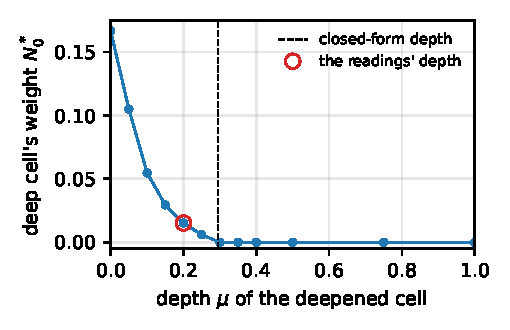
\includegraphics[width=\columnwidth]{../../build/figures/deep-cell-weight.pdf}
  \caption{A deep enough cell loses its weight, falling on a ring of \val{ringCells} qubits from its uniform share to zero at depth \val{dropDepth}, where the other cells, optimized without it, first hold it at their common value. The dashed line is that depth in closed form, Eq.~\eqref{eq:depth}, and the open circle marks depth \val{ringShallowDepth}, where the readings are made.}
  \label{fig:deep}
\end{figure}

\section{Across models and sizes}
\label{sec:breadth}

Beyond the ring, the code solves a catalogue of models, at the breadth printed here, which the code calls its survey grade, and a wider catalogue whose results are stored with the code (Sec.~\ref{sec:limits}). The catalogue varies the family of pieces, the lattice, the coupling's sign, a longitudinal field and which cell is deepened (Table~\ref{tab:catalogue}, Appendix~\ref{app:models}). Its breadth is in kinds of model, so no model has more than \val{catalogueLargest} cells, and the general claims hold at every size.

\begin{table*}[tp]
  \caption{In the catalogue, by kind of model, Places below counts the places below the common value by more than \val{catalogueBelowMargin} before any cell is deepened, with models that differ only in which cell would be deepened counted once. Every such place carries no weight. The last two columns concern the cell deepened to depth \val{catalogueDeepDepth}, among the models where the solver's weighting gave it weight before: those it drops out of, and the largest weight it keeps where it does not.}
  \label{tab:catalogue}
  \small
  % GENERATED from src/saddle/tables.py by `make generate`; edit the source, not this file.
\begin{tabular}{llcp{2.45in}rrrr}
\toprule
Pieces & Lattice & Cells & Parameters & Models & Places below & Drops out & Weight kept \tabularnewline
\midrule
Ising & ring & $3$--$5$ & $g$ $=$ $0.5$, $1$, $2$, $J$ $=$ $1$; $g$ $=$ $0.5$, $1$, $2$, $J$ $=$ $-1$; $g$ $=$ $0.5$, $1$, $2$, $J$ $=$ $1$, $b$ $=$ $0.5$ & $27$ & $0$ & $27$ of $27$ & --- \tabularnewline
Ising & open chain & $3$--$5$ & $g$ $=$ $0.5$, $1$, $2$; $J$ $=$ $1$; deepening an end or the middle & $18$ & $18$ & $9$ of $9$ & --- \tabularnewline
Ising & two-leg ladder & $6$ & $g$ $=$ $0.5$, $1$, $2$; $J$ $=$ $1$ & $3$ & $2$ & $3$ of $3$ & --- \tabularnewline
Ising & complete graph & $4$--$5$ & $g$ $=$ $0.5$, $1$, $2$, $J$ $=$ $1$; $g$ $=$ $0.5$, $1$, $2$, $J$ $=$ $-1$ & $12$ & $0$ & $12$ of $12$ & --- \tabularnewline
Ising & star & $4$--$5$ & $g$ $=$ $0.5$, $1$, $2$; $J$ $=$ $1$; deepening the hub or a leaf & $12$ & $6$ & $6$ of $6$ & --- \tabularnewline
XXZ & ring & $3$--$5$ & $\Delta$ $=$ $-0.5$, $0.5$, $1.5$; $J$ $=$ $1$; $b$ $=$ $0.2$ & $9$ & $0$ & $5$ of $9$ & $0.029$ \tabularnewline
XXZ & open chain & $3$--$5$ & $\Delta$ $=$ $-0.5$, $0.5$, $1.5$; $J$ $=$ $1$; $b$ $=$ $0.2$; deepening an end or the middle & $18$ & $9$ & $8$ of $15$ & $0.073$ \tabularnewline
XXZ & star & $4$--$5$ & $\Delta$ $=$ $-0.5$, $0.5$, $1.5$; $J$ $=$ $1$; $b$ $=$ $0.2$; deepening the hub or a leaf & $12$ & $6$ & $6$ of $6$ & --- \tabularnewline
random & random graph & $3$--$5$ & $3$ draws & $9$ & $15$ & $3$ of $5$ & $0.041$ \tabularnewline
\midrule
All &  & $3$--$6$ &  & $120$ & $56$ & $79$ of $92$ & $0.073$ \tabularnewline
\bottomrule
\end{tabular}

\end{table*}

% claims: catalogue.general
Every computed pair meets the general claims across the catalogue, a check of the computation against the theorems. In \val{catalogueModels} models of \val{catalogueFamilies} families on \val{catalogueLattices} lattices, before any cell is deepened, the state side and the weighting side reach one value to the bound \val{catalogueGapBound}, and every model meets the four conditions to the bounds of their residuals, the difference between the two programs' values, not the conditions, certifying each pair. Of the places, \val{catalogueBelowPlaces} fall short of the common value by more than \val{catalogueBelowMargin}, and each carries a weight below \val{catalogueNoWeightBound}. In every model the first place's weight lies between its two one-sided rates, as Proposition~\ref{prop:rates} requires of every optimal weighting, and each of the \val{catalogueUniformRings} systems a rotation maps into itself, a uniform ring or a complete graph, reaches its ground energy per cell.

% claims: catalogue.deep
Whether a deepened cell drops out depends on the family. Counting only cells the solver's weighting gave weight before deepening, a cell deepened to depth \val{catalogueDeepDepth} drops out of \val{catalogueIsingDropped} of the \val{catalogueIsingModels} such Ising models, whatever the lattice, the coupling's sign or the cell deepened, and of only \val{catalogueOtherDropped} of the \val{catalogueOtherModels} XXZ and random ones, keeping a weight of up to \val{catalogueKeptLargest} in the rest. Where the optimum is a set, as on the open Ising chains and stars, some optimal weighting gives the cell none even before it is deepened, so there its dropping out shows little. The rings among those are taken up below. Why the cell keeps its weight on the open XXZ chains and random graphs where it does is not studied here.

% claims: unique.catalogue
Whether the optimal weighting is unique sorts the catalogue three ways. Counting each model before its cell is deepened and after, so that an open chain or a star appears once for each cell it deepens, \val{uniqueCertified} of the \val{uniqueModels} meet Proposition~\ref{prop:single}'s condition at the computed weighting, so their weighting is unique, counting a lowest level as single only when the next lies more than \val{uniqueGap} above it and a curvature as negative only when it lies more than \val{uniqueCurve} below zero. In \val{uniqueNarrow} more the lowest level at the optimum is not single, where the floor has a corner, and no weight's spread exceeds the bound \val{uniqueSpreadBound} over the weightings within \val{uniqueNear} of the common value. In the remaining \val{uniqueWide} some weight spreads by more than that bound. Among them the optimum is a set wherever two places each hold the common value up unaided, so that the weight between them is free, as in every open Ising chain and every Ising star before any cell is deepened. In the others a wide spread could come from a set or from a single optimum whose floor is very flat.

% claims: scaling.ising
The general claims hold at every size, so only a family's particular findings, such as the drop-out, can change with size, and I follow the drop-out. With the ring's couplings, $g = J = 1$, on Ising rings of \val{scalingSmallest} to \val{scalingLargest} cells the deepened cell drops out at every size, at a depth rising from \val{scalingFirst} to \val{scalingLast}.

% claims: scaling.weighting
The weighting side reaches larger rings, because the drop-out is decided by the other cells' optimum alone, in which the depth does not appear, and on the transverse-field ring Eq.~\eqref{eq:depth} turns that optimum into the drop-out depth in closed form (Appendix~\ref{app:dropout}). The other cells' optimal weighting is found by maximizing their floor over weightings with a sequential quadratic program, each floor computed by a sparse eigensolver in the deep cell's spin-up sector. Computed this way on rings of \val{depthsSmallest} to \val{depthsLargest} cells, the depth rises from \val{depthsFirst} to \val{depthsLast}, each step adding less than the one before, the last \val{depthsLastStep}. It agrees with the state-side depths up to \val{scalingLargest} cells to the bound \val{depthsAgreementBound}. A fit of the form $\mu_\infty - a\,n^{-p}$ puts its limit at \val{depthsLimit} over the sizes from \val{depthsFitFrom}, with $p = \val{depthsPower}$, and at \val{depthsLimitLate} over those from \val{depthsFitFromLate} (Fig.~\ref{fig:size}a). The limit is a fit's, not a result, and the larger rings below show that the difference between the two windows understated its uncertainty.

% claims: depths.free
Free fermions reach far larger rings. With its weight at zero the deepened cell's field drops out, so its spin is conserved, and the other cells' weighted Hamiltonian is still quadratic in Majorana operators. Its lowest level is the pair of Eq.~\eqref{eq:depth}: the ground state of the even fermion-parity sector, and that state's image under the deepened spin, which carries one sector to the other at the same energy. So the other cells' floor is the even sector's, Eq.~\eqref{eq:freefloor}, and Eq.~\eqref{eq:depth}'s two numbers, the deepened cell's half-link energy $d$ and the pair's off-diagonal $\xi$, come from that sector's correlations (Appendix~\ref{app:dropout}). Computed this way on rings of \val{largeSmallest} to \val{largeLargest} cells, which Appendix~\ref{app:models} lists, each optimum certified by the bracket to the bound \val{largeGapBound}, the depth meets the sequential quadratic depths to within \val{largeAgreementBound} up to \val{largeSharedLargest} cells. It rises to \val{largeDepthLast} at \val{largeLargest} cells, each doubling of the size adding about \val{largeDoublingShare} of what the doubling before it added (Fig.~\ref{fig:size}a). At every size the even sector's lowest level is single and the other cells' floor curves down in every direction at their optimum, so Eq.~\eqref{eq:depth}'s hypotheses hold and their optimal weighting is unique. The same fit from \val{largeFitFrom} cells puts the limit at \val{largeLimit}, with $p = \val{largePower}$, and from \val{largeFitFromLate} cells at \val{largeLimitLate}, below the small rings' limit by several times the difference between their two windows, and $p$ drifts with the window and the sizes in it. The bracket certifies the other cells' value, not the depth, which depends on their optimal state too and is certified less tightly, so neither the last doublings' small steps nor the depths' last figures on the largest rings are certified: the powers are descriptive, and this limit too is a fit's.

% claims: parity.rings
An even size of XXZ ring keeps the deepened cell, under Proposition~\ref{prop:parity}'s hypotheses and to first order in the field, and an odd size leaves the outcome to the drop-out criterion. Their couplings conserve the magnetization $M = \sum_x Z_x$ and are unchanged by flipping every spin. On an even ring whose other cells have a unique optimal state, with $M = 0$, and under the further hypotheses of Proposition~\ref{prop:parity}, a deepened cell, to first order in a small uniform field, never drops out, and as the depth grows its weight times its depth tends, wherever the other weights settle, to the field times a signed mean of the other cells' weights, each weighted by how strongly its spin moves the deepened one's, Eq.~\eqref{eq:law}: the field on the other cells turns the deepened spin against its own field, so no state optimal for the others gives it a positive spin. No such argument applies on an odd ring, and the criterion applies as it stands: the cell drops out at a finite depth exactly when some state optimal for the others gives its spin a positive expectation. On the ring of three cells the others' optimal states form a pair of opposite magnetizations, which the field does not split, and one of them gives the deepened spin that expectation.

% claims: scaling.xxz
At one anisotropy the computed rings follow the parity (Fig.~\ref{fig:size}b, c). Their couplings are $J = 1$ and $\Delta = \val{xxzAnisotropy}$, the field is swept from \val{xxzFieldLeast} to \val{xxzFieldMost}, and the depth up to \val{xxzDeepest}. The drop-out depths and the curves of Fig.~\ref{fig:size}b, c are at the field \val{xxzCurveField}. The deepened cell drops out on the odd XXZ rings of \val{scalingSmallest} to \val{scalingLargest} cells, at depth \val{xxzOddFirstDepth} on \val{xxzOddFirstCells} cells and \val{xxzOddLastDepth} on \val{xxzOddLastCells}. It never drops out on the even rings, where no state optimal for the other cells gives its spin a positive expectation, so the criterion's program has no solution, and at every depth sampled up to \val{xxzDeepest} its weight falls as the inverse of the depth, the product settling near \val{xxzKappaFirst} on \val{xxzEvenFirstCells} cells and \val{xxzKappaLast} on \val{xxzEvenLastCells}. The weight on an odd ring reaches zero at the depth where the common value meets the other cells' value and stops falling.

% claims: scaling.odd
Across anisotropies the odd rings do not all drop out. On odd XXZ rings of \val{xxzOddFirstCells} and \val{xxzOddLastCells} cells at four anisotropies from \val{xxzOddDeltaLeast} to \val{xxzOddDeltaMost}, those of Table~\ref{tab:catalogue} and the isotropic point, and the field \val{xxzCurveField}, the other cells' optimal states are found directly: their weighted Hamiltonian's ground level is one state of magnetization $\pm 1$ or a pair of the two, every density conserves the magnetization, so a state's densities there depend only on its share of positive magnetization, and the bounds on their densities fix that share. The deepened cell drops out on \val{xxzOddDropped} of the \val{xxzOddRings}. The bounds fix the share at \val{xxzKeptShare} on the ring of \val{xxzKeptCells} cells at $\Delta = \val{xxzKeptDelta}$, where the deepened spin is \val{xxzKeptSpin}, turned against its field, so the cell never drops out: at depth \val{xxzDeepest} its weight times its depth is \val{xxzKeptProduct}, and the common value stays \val{xxzKeptLift} above the other cells' value. The parity settles the outcome on even rings, and the other cells' optimal states settle it on odd ones.

% claims: scaling.law
At the weakest field the even rings' weight times depth, read at the deepest depth computed, \val{xxzDeepest}, where it has nearly settled (Fig.~\ref{fig:size}c), with the other cells' weights read there, differs from its derived limit by as much as \val{xxzLawGap}, and it follows the field in proportion to within \val{xxzFieldSpread}, though the law does not require proportion, since the other cells' weights move with the field. At that depth most of the gap is the finite depth's. On \val{xxzEvenFirstCells} cells, at every field, the product is the law times $\mu/(\mu + b)$ to the bound \val{xxzDepthFactorBound}, so the gap there, $b/(\mu + b)$, closes as the depth grows, while on \val{xxzEvenLastCells} cells, with that factor divided out and the law's responses and weights both read at that depth, \val{xxzDepthLeftLeast} to \val{xxzDepthLeftMost} is left, growing with the field, as a law first order in the field allows.

% claims: exits.conservation
The proposition needs the magnetization conserved, but the outcome, in the cases computed, does not. With a transverse field of up to \val{exitTransverseField} on every cell, which breaks the conservation, the even ring's deepened cell still does not drop out at any depth sampled.

\begin{figure*}[tp]
  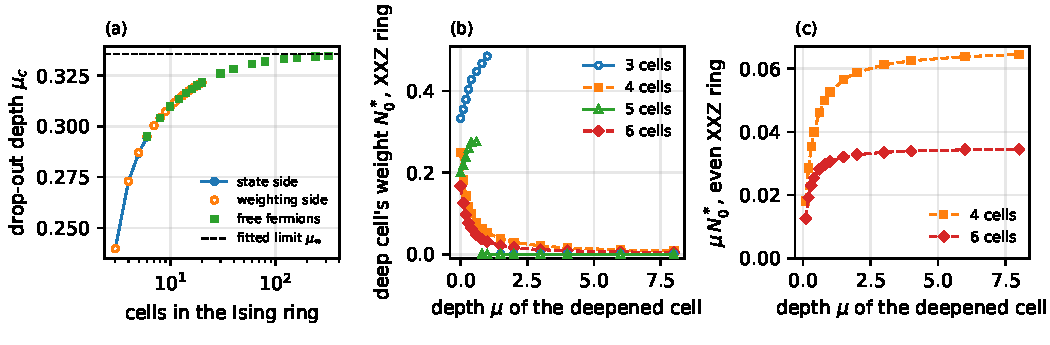
\includegraphics[width=\textwidth]{../../build/figures/size.pdf}
  \caption{Size. (a) The depth at which a deepened cell drops out of an Ising ring rises with the ring's size and levels off: computed by the state-side program to a stated tolerance up to six cells (filled), in closed form from the weighting side up to \val{depthsLargest} (open), and by free fermions up to \val{largeLargest} (squares), with the limit fitted from \val{largeFitFromLate} cells (dashed), whose power moves with the window and with the largest rings' depths. (b) The weight of a deepened cell on XXZ rings against its depth, at field \val{xxzCurveField}. On odd rings (solid) it first grows as the deepened spin turns along its field, while the common value, which falls with depth at the weight times that spin where the optimum is unique, bends down toward the other cells' level. Where it meets that level the common value stops falling, so the weight reaches zero there, between two sampled depths (Proposition~\ref{prop:dropout}); the samples do not show whether it falls there at once or continuously. On even rings (dashed) it falls without reaching zero. (c) On even rings, the weight times the depth, which settles: the weight falls as the inverse of the depth.}
  \label{fig:size}
\end{figure*}

\section{The whole's frame}
\label{sec:frame}

% claims: saddle.evolution
The readings of time below build on one more consequence of the saddle of Sec.~\ref{sec:saddle}. The first condition of Eq.~\eqref{eq:conditions} has the weighted Hamiltonian hold the saddle state at the common value, $A_{N^*}\rho^* = e^*\rho^*$, so the two commute and the state is unchanged by $e^{-iA_{N^*}t}$ (Corollary~\ref{cor:evolution}). With the canonical densities, $A_{N^*}$ runs each place's own piece at that place's weight and each link at the mean weight of its two ends, Eq.~\eqref{eq:evolution}. A place with no weight contributes none of its own pieces, and only its links act on it, each at half its neighbour's weight.

% claims: signals.wall
What the weighted Hamiltonian leaves out is exact. A link whose two places both carry no weight has no term in it, and a weightless place whose links all join weightless places appears in no term at all (Corollary~\ref{cor:crossing}). Where the pieces act on one place or two, such a place is left untouched, and where such places cut the system in two, nothing on one side reaches the other.

Rates are rates against some time, and nothing outside a closed system keeps one. Whatever time a part of it has must be read from a clock among its parts, and its rates at each place from probes there:

\premise{probes}

% claims: probes.idle
Identical idle probes, one at every place, leave the saddle where it is, shifting the common value by their ground energy and leaving every optimal weighting optimal (Lemma~\ref{lem:probes}), because each probe adds its energy at its place's weight and the weights sum to one. Under $A_{N^*}$ each probe then turns by its weighted energy alone.

Every reading of time uses one further premise, and no proposition does. It defines the whole's frame, the system with its probes and a clock, stationary as one.

\premise{evolution}

Like the saddle, the premise is a condition the whole satisfies, not a state it is brought to.

% claims: evolution.conditioned
Conditioned on its clock, the system evolves under the weights. Let the whole be the system with its probes and a clock with energy $H_C$, stationary under $A' + H_C$, where $A' = \sum_x N^*_x D'_x$ counts each probe's energy in its place's density. Then the rest, conditioned on the clock's reading $t$, is the rest at reading zero evolved by $e^{-iA't}$, up to a phase (Proposition~\ref{prop:conditioned}, Eq.~\eqref{eq:conditioned}). Running the rest forward is running the clock back, because the two energies act on different parts. This is Page and Wootters' construction~\cite{PageWootters1983}, with the weighted Hamiltonian in place of the Hamiltonian. It is one of three equivalent formulations of relational dynamics~\cite{HoehnSmithLock2021}, and in it clocks that are the internal degrees of freedom of relativistic particles read time dilation from their motion~\cite{SmithAhmadi2020}. A clock's proper time along two paths can be read as lost interference~\cite{ZychEtAl2011}, and clocks whose mass-energy gravitates entangle through time dilation~\cite{CastroRuizEtAl2017}. Here the clocks' rates come from the weights.

% claims: timeless.rates
A computation with no time in it shows the rates. I solve the ring of \val{timelessCells} cells, its first cell at depth \val{timelessDepth}, together with a probe at every place and a clock, once, as one stationary state, by projecting a starting state onto the states the stationarity condition allows, and a reading $t$ enters only through the clock state one conditions on. Conditioned on the clock's readings, every probe turns at its place's weight to within half the clock's resolution, the largest gap falling from \val{timelessGapFirst} with \val{timelessLevelsFirst} levels to \val{timelessGapLast} with \val{timelessLevels} (Fig.~\ref{fig:timeless}). By Proposition~\ref{prop:conditioned} the rates are the weights exactly for an exactly stationary whole, so the gap is not evidence for the rates. It measures how far the computed whole, cut from a product of states to the energies that cancel within half the resolution, falls short of stationary, and the computation shows that a clock of finitely many levels reads the rates to within its resolution. Past its drop-out the deep cell's weight is set to zero, as Proposition~\ref{prop:dropout} gives it, and its probe then turns at a rate below the bound \val{timelessStoppedBound}: the stopped clock is the proposition's, not the computation's. The time-stepped simulations used below are this computation's limit as the clock's resolution becomes finer, and cost less.

\begin{figure*}
  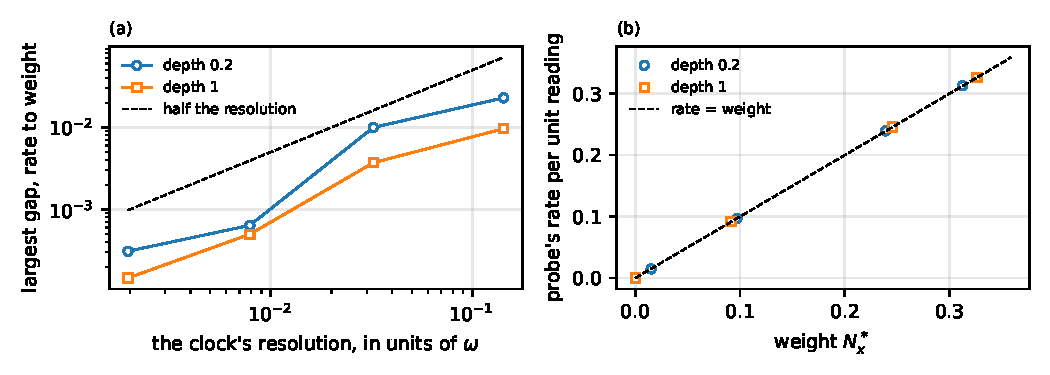
\includegraphics[width=\textwidth]{../../build/figures/timeless.pdf}
  \caption{Time read from a clock inside the whole, solved once with no time parameter. (a) The largest gap between a probe's rate and its place's weight, against the clock's resolution, the spacing of its levels: it lies within half the resolution and falls with it overall. (b) At the finest clock every probe turns at its place's weight, and past the deep cell's drop-out its probe does not turn.}
  \label{fig:timeless}
\end{figure*}

\section{The lapse read from inside the system}
\label{sec:readings}

Under the premises of the whole's frame the weights can be read. A reading identifies a computed quantity with a physical one and states any premise the identification needs, and is never a claim. Each quantity comes from simulating the system and is read off the simulated signal, not inferred from the law it should satisfy (Table~\ref{tab:readings}).

\begin{table*}[tp]
  \caption{The readings. A matched reading's quantity, computed from the system, takes the value its identification gives; a reading is the identification alone, its quantity computed under its premises. The shadow price is read in Sec.~\ref{sec:forbids}.}
  \label{tab:readings}
  \footnotesize
  % GENERATED from src/saddle/tables.py by `make generate`; edit the source, not this file.
\begin{tabular}{p{1.0in}llp{2.1in}p{2.8in}}
\toprule
\raggedright Reading & Standing & Premises & \raggedright Quantity & \raggedright As simulated \tabularnewline
\midrule
\raggedright Clock & reading & \ref{premise:evolution}, \ref{premise:probes} & \raggedright the rate of a test clock's phase at each place per unit of the clock's reading, in units of its frequency & \raggedright Every simulated clock runs at its place's weight, to within $10^{-9}$. On the ring of $6$ qubits the first cell's clock runs at $0.015$ at depth $0.2$, and past its drop-out, at depth $1$, it stops; on the even XXZ ring of $4$ cells the deepened cell's clock still runs at depth $8$, at $0.0081$. \tabularnewline
\raggedright Chance from records & reading & \ref{premise:evolution}, \ref{premise:records} & \raggedright the CHSH value of Alice's and Bob's outcomes against the overlap of the outside copy of the friends' records & \raggedright Solved once with no time parameter, the protocol's CHSH value is $(1+\gamma)^2/\sqrt{2}$ to within $10^{-9}$, from $2.828$ with no copy to $0.7071$ with a full one, above the bound $2$, with these settings, only while the overlap exceeds $0.6818$ (with turned settings, derived rather than simulated, at every overlap short of a full copy); nothing signals, to the bound $10^{-12}$. \tabularnewline
\raggedright Lapse & matched & \ref{premise:evolution}, \ref{premise:probes} & \raggedright the energy an excitation at a place adds to the weighted generator, per unit of its own energy & \raggedright Exciting the probe at each place of the ring adds its place's weight times the probe's energy, to within $10^{-12}$ of the weight. \tabularnewline
\raggedright Tolman temperature & matched & \ref{premise:evolution}, \ref{premise:probes}, \ref{premise:equilibrium} & \raggedright the temperature a test thermometer reads at each place, in units of the global temperature & \raggedright Every simulated thermometer reads a temperature times weight equal to the global temperature, to within $10^{-9}$; at depth $0.2$ the first cell runs $11$ times hotter than a cell of the uniform ring, and past its drop-out its thermometer has no finite reading. \tabularnewline
\raggedright Proper length & matched & \ref{premise:evolution}, \ref{premise:probes}, \ref{premise:cone} & \raggedright the time a long wave takes to cross a stretch, read by the clocks along it, and the ground state's entanglement across a cut & \raggedright Long waves on the weighted chain take the optical time to within the relative bound $0.001$, and the saddle state's own entanglement is the vacuum's on the metric whose lapse is its weights, with a cutoff of one cell, to within $10^{-4}$. \tabularnewline
\raggedright Horizon & reading & \ref{premise:evolution}, \ref{premise:probes}, \ref{premise:equilibrium} & \raggedright at a place with no weight, its clock's rate, its thermometer's reading, and the energy its excitation adds to the whole & \raggedright Past its drop-out the first cell's simulated clock stops, its thermometer has no finite reading, and an excitation there adds nothing to the weighted generator's energy. \tabularnewline
\raggedright Cosmological constant & reading & \ref{premise:constant} & \raggedright the part of the common value set by the size of a uniform critical ring, and the central charge it gives & \raggedright On uniform critical rings of $8$ to $60$ cells the size-set part gives a central charge $0.5000$, and an interval's entanglement entropy gives $0.5003$ independently. \tabularnewline
\raggedright Horizon temperature & matched & \ref{premise:subsystem}, \ref{premise:cone} & \raggedright the ratio of a part's horizon temperature, the speed times its weights' slope at the edge over 2 pi, to the local temperature at its centre & \raggedright For intervals of $8$ to $40$ cells of the critical chain, the ratio read with the weights' longer-range terms differs from one by $1.4\times10^{-4}$ to $5.6\times10^{-6}$; from the nearest terms alone it is $1.05$. \tabularnewline
\raggedright De Sitter temperature & reading & \ref{premise:subsystem}, \ref{premise:cone}, \ref{premise:patch} & \raggedright the temperature of the cosmological horizon, for the measured cosmological constant & \raggedright Not simulated: the system supplies the 2 pi. With the measured Hubble rate $67.36$ km/s/Mpc and dark-energy fraction $0.6847$, the temperature is $2.20\times10^{-30}\,\mathrm{K}$, with the $1\%$ uncertainty those values carry. \tabularnewline
\raggedright Shadow price & matched & none & \raggedright the rate at which the common value moves when one place's bound is relaxed & \raggedright Relaxing and tightening each cell's bound on the ring and solving again moves the common value, between the two, at that cell's weight, to within $10^{-4}$. \tabularnewline
\bottomrule
\end{tabular}

\end{table*}

The identification the readings make is with the lapse of a static spacetime~\cite{ArnowittDeserMisner2008,Gourgoulhon2007}. There the lapse multiplies the local energy density inside the generator of time, and it fixes three local things: how fast proper time runs against the time far away, what share of a local energy is seen far away, and the temperature of equilibrium. The weights do the first two under the frame's two premises, and the third under a premise of equilibrium. Two differences stand from the start. In gravity the local energies vanish on physical states, so every lapse describes the same physics and its choice is a gauge. Here the densities neither vanish nor commute, so different weightings generate different evolutions, and the premise of evolution says which one a part reads. And since the weights sum to one, only their ratios carry physics; unlike a lapse normalized at a reference observer, places far away, added without interacting, leave the weights as they were or take them all, unless the two common values tie: of two systems that do not interact, every optimal weighting puts all its weight on the one with the higher common value. The analogy is kinematic, since every weighting multiplies the local energies inside a generator, and no field equation ties the weights to the energy's distribution here. Gravity's local constraints have also been replaced by a single one, Thiemann's master constraint, the integral of their squares, which vanishes exactly when every one of them does~\cite{Thiemann2006}. The saddle's single condition is instead a common bound, met without any local energy vanishing, with the weights that certify it.

\subsection{Clock rate, redshift and temperature}
\label{sec:lapse}

Under the frame's premises each weight is its place's clock rate. The probe at $x$, an idle qubit of frequency $\omega$, gains phase at
\begin{equation}
  \frac{d\phi_x}{dt} = N^*_x\, \omega
  \label{eq:clockrate}
\end{equation}
per unit of the reading of the clock among the whole's parts: local time at $x$ runs at its weight, as proper time runs at the lapse. Every clock on the uniform ring runs at one over the number of cells. The simulation reads each rate off its probe's phase and finds it at its place's weight to the bound \val{clockRateGapBound} (Fig.~\ref{fig:simulation}a). With the first cell of the ring of \val{simCells} cells at depth \val{simShallowDepth}, its clock runs at \val{deepClockShallow}, and at depth \val{simDeepDepth}, past its drop-out, it stops. The deepened cell's clock on the even XXZ ring of \val{xxzSimCells} cells still runs at depth \val{xxzSimDepth}, at \val{xxzDeepClock}.

\begin{figure}[!tbp]
  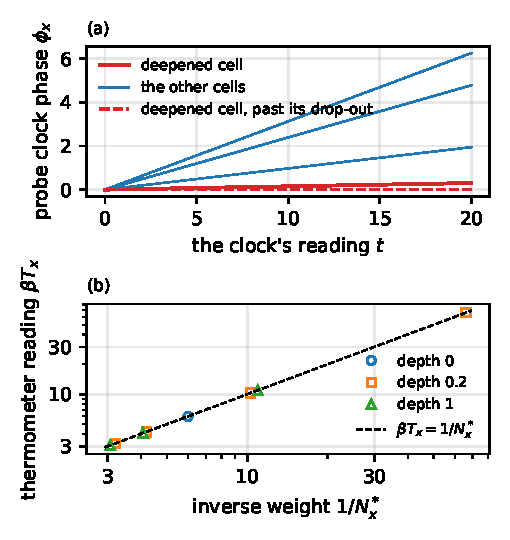
\includegraphics[width=\columnwidth]{../../build/figures/simulation.pdf}
  \caption{The lapse's rates, simulated. (a) The clocks on the ring with the first cell at depth \val{simShallowDepth}: each runs at its cell's weight, the deep cell's slowest, and past the deep cell's drop-out (dashed) its clock stops. (b) Probe thermometers at every depth simulated, against the inverse weight: every reading sits on Tolman's line; a cell past its drop-out has no finite reading and is not shown.}
  \label{fig:simulation}
\end{figure}

Each weight is also its place's redshift. Exciting the probe at place $x$ by an energy $\Delta e_x$ raises the weighted Hamiltonian's energy by
\begin{equation}
  \Delta E = N^*_x\, \Delta e_x ,
  \label{eq:redshift}
\end{equation}
so the energy a probe's excitation adds to the whole is the probe's energy times its place's weight, as a lapse scales a local energy seen from far away. An excitation of a cell's own pieces changes its neighbours' densities too, through the links. The simulation excites the probe at each place of the ring and finds the added energy at its weight times the probe's energy, to the bound \val{redshiftGapBound}. Both readings rest on the premises of evolution and probes, and neither on equilibrium. Under those premises the relations are identities of the weighted Hamiltonian, and the simulation shows that the computed signals carry them.

Every weighting has these properties toward the weighted Hamiltonian it defines. What the saddle adds is which weightings: one where the optimum is unique, and a set where it is not, as on the open chain (Sec.~\ref{sec:readings-space}).

Temperature, the third thing a static lapse fixes, needs equilibrium:

\premise{equilibrium}

A probe thermometer at $x$ then reads
\begin{equation}
  T_x = \frac{1}{\beta N^*_x}, \qquad T_x N^*_x = \frac{1}{\beta},
  \label{eq:tolman}
\end{equation}
so temperature times weight is one constant across the system: a place with less weight runs hotter, without bound as its weight goes to zero. Tolman's relation for a static field has this form~\cite{Tolman1930}; here it is an identity of the weighted Hamiltonian and the probes under the premise, where Rovelli and Smerlak derive it with temperature the rate of thermal time~\cite{RovelliSmerlak2011}. On a lattice in a thermal state a temperature belongs to a block, not a cell: the state factors into blocks of one temperature only above a least block size~\cite{HartmannMahlerHess2004}, and a temperature is shown to be local above a threshold temperature~\cite{KlieschEtAl2014}. The probe thermometers read one cell's under the premise of equilibrium, which is stated, not derived. Every simulated thermometer reads a temperature times weight equal to the global temperature, to the bound \val{tolmanGapBound}, and at depth \val{simShallowDepth} the first cell runs \val{deepHotRatio} times hotter than a cell of the uniform ring (Fig.~\ref{fig:simulation}b).

% claims: equilibrium.coldest
The weights' proportions appear again from maximum entropy, with no generator of time. Bound every local energy by one common level above the common value, and take the state of greatest entropy within the bound~\cite{Jaynes1957,Jaynes1957b}: it is thermal in the local energies weighted by its multipliers, the Lagrange multipliers of the bounds. As the level falls to the common value the multipliers grow without bound in the proportions of the saddle weights, wherever the optimal weighting is unique (Proposition~\ref{prop:coldest}), so the saddle weights are the shape of the coldest equilibrium such a bound allows. Maximum-entropy inference from local expectations can jump where the local states change smoothly~\cite{ChenEtAl2015}, whereas here, as the bound falls, its multipliers settle. As the level's height above the common value falls from \val{coldestFirstGap} to \val{coldestLastGap} on the ring of \val{coldestCells} cells deepened to \val{coldestDepth}, the multipliers' total climbs from \val{coldestFirstTotal} to \val{coldestLastTotal}, and their largest distance from the weights' proportions shrinks from \val{coldestFirstDistance} to \val{coldestLastDistance}. The approach is slow, and at the nearest level computed the distance still exceeds the deep cell's weight, \val{deepClockShallow}. The proof bounds how far the proportions' floor sits below the common value, by the logarithm of the dimension over the multipliers' total. It does not bound how far the proportions sit from the weights, which would need the floor's curvature at its maximum, so it gives no rate for the distance.

% claims: coldest.symmetric, coldest.chain
Where the optimum is a set, the limit can still be one point. The optimal weightings of the open chain of \val{coldestChainCells} cells form a segment, the weight split freely between the two ends, and the chain's reflection maps the densities onto one another. Every coldest equilibrium is then symmetric, so every limit point of its proportions is the segment's one symmetric point, the even split (Corollary~\ref{cor:symmetric}). As the height above the common value falls from \val{coldestFirstGap} to \val{coldestLastGap}, the proportion at each end rises from \val{coldestChainFirstEnd} to \val{coldestChainLastEnd}, the two ends equal throughout. The even split the open chain's signals use is thus also the coldest equilibrium's limit.

% claims: exits.degenerate
The limit requires that some optimal weighting's weighted Hamiltonian not be a multiple of the identity. When every density is a multiple of the identity, the multipliers stay below the bound \val{exitIdentityBound} at every level computed.

Gravity's lapses and these weights differ in where they come from. A slicing condition fixes the lapse of canonical gravity. A symmetry, a timelike Killing field, fixes a static lapse up to a constant, as in Tolman's equilibrium and in the accelerated frame~\cite{Tolman1930,BisognanoWichmann1976}. Here the energies fix the weights through the saddle, normalized to sum to one: one weighting where the optimum is unique, and a convex set of them where it is not, as on the open chain.

\subsection{The spatial part}
\label{sec:readings-space}

The clocks give the time part of a geometry, and signals give its spatial part. In a static field light's coordinate speed is the lapse divided by the scale of the spatial metric~\cite{Gourgoulhon2007}, so once the clocks have fixed the lapse, the time a signal takes to cross a place measures how long the place is. Lengths rest on a premise about long waves, packets many cells wide with no carrier, so that every wavelength in them is long against a cell:

\premise{cone}

Under the premise a cell's proper length is its radar length, the speed of light times the time long waves take to cross it, read by the clock at the cell. Near any place the weighted chain is the uniform chain with that place's clock slowed by its weight, still critical to leading order in the weights' gradient, so its long waves cross each cell in the same time read there: every cell has the same proper length whatever its weight, and the weights enter the geometry only as its lapse,
\begin{equation*}
  ds^2 = -\big(vN(x)\big)^2 dt^2 + dx^2 ,
\end{equation*}
with $x$ counted in cells. Space is the description's, flat in its cells; the whole adds only how fast each place's time runs. Distances read in the whole's time are optical, the time a long wave takes,
\begin{equation}
  t = \sum_x \frac{1}{vN(x)} ,
  \label{eq:optical}
\end{equation}
summed over the cells crossed: they stretch where the weights are small and diverge where the weights vanish, while distances summed cell by cell, each read by the clock at its cell, do not stretch. This is the metric conformal field theory gives a critical chain whose couplings vary in space~\cite{DubailEtAl2017}, and the form a horizon simulated on a lattice takes~\cite{RodriguezLagunaEtAl2017}. Position-dependent hoppings also put lattice Dirac fermions in a curved spacetime, Rindler's among them~\cite{BoadaEtAl2011}. The reading adds that the lapse is the saddle's weights.

% claims: space.waves
The long waves bear it out on weightings chosen by hand. On the critical chain of \val{spaceCells} cells weighted uniformly, falling to \val{spaceFallMin}, and in a well down to \val{spaceWellMin}, Gaussian packets of long waves \val{spaceWidth} cells wide, timed by when their centre, the mean position of their squared amplitudes, crosses each end, take the optical time to within the relative bound \val{spaceWaveBound}, Eq.~\eqref{eq:optical} taken as an integral with the weights read linearly between cells, since the ends fall between them, and read by the clock at each place they move at $v$ to within the relative bound \val{spaceSpeedBound}. Narrower packets depart more, by the lattice's dispersion. Toward a zero of the weights, $N = \kappa r$ at a distance $r$ from it, the time grows as $\ln(r_1/r_2)/(v\kappa)$ to within the relative bound \val{spaceZeroBound}, so the time to reach the zero diverges, as the time to reach a horizon does. A sharp step between weights one and \val{spaceStepWeight} turns back \val{spaceStepShare} of a packet \val{spaceWidth} cells wide, by its squared amplitude, where a continuum would turn back nothing: the geometry is met at a resolution.

% claims: signals.stop
Where the weights vanish over a stretch, the reading has no length to give, and the open chain's saddle has such a stretch. The saddle leaves every cell between the two ends of the open transverse-field chain of \val{signalCells} cells without weight, because an end's density holds half of one link and an interior cell's density halves of two. The split between the ends is free, because their densities act on different cells, so every weighting $(a, 0, \dots, 0, 1-a)$ with $a$ between zero and one is optimal, a segment rather than a point. Along weightings from uniform toward the even split the interior cells share one weight $w$, and a disturbance at the first interior cell takes a span going as $w$ to the power \val{signalExponent} to reach the last, the span being the time until the last cell's density moves by a set departure. The span times the weight stays near \val{signalCrossing}, its relative spread below the bound \val{signalCrossingSpreadBound}. Along this family the interior's dynamics is, apart from the links to the two ends, the unweighted interior's rescaled by $w$, so the exponent illustrates the rate rather than testing it. At the even split, watched over a window of \val{signalWindow}, no density beyond the kicked cell moves by more than the bound \val{signalWallBound}: the disturbance never travels into the chain past the cell it starts in. That is exact, since no term of the weighted Hamiltonian reaches past the kicked cell (Corollary~\ref{cor:crossing}), and the computation confirms it.

% claims: space.entanglement
The stationary whole carries the metric of Eq.~\eqref{eq:optical} with no clock at all. Across every cut of such a chain's ground state the entanglement is the conformal vacuum's on the metric, with one cell as the cutoff,
\begin{equation}
  S(x) = \frac{1}{12} \ln\!\Big[\frac{2\tilde L}{\pi} \sin\frac{\pi \tilde x}{\tilde L}\; vN(x)\Big] + \text{const},
  \label{eq:vacuum}
\end{equation}
with $\tilde x$ the cut's optical position, $\tilde L$ the chain's optical length and $1/12$ a sixth of the chain's central charge: in words, the vacuum's entropy in optical coordinates, each cut's cutoff one cell of proper length, which is $1/(vN)$ of optical length. It holds on \val{spaceEntropyCells} cells, smooth or with smoothed steps, to the bound \val{spaceEntropyBound}, with nothing fitted: the uniform chain's departure from Eq.~\eqref{eq:vacuum}, cut by cut, its constant, its end terms and its alternation between neighbouring cuts, is carried to the weighted chain at the same cut, and the cuts within a tenth of the chain of either end are left out. Fitted freely, the power of the weight at the cut lies between \val{spacePowerLow} and \val{spacePowerHigh}. Of the metrics that share the long waves' light cones, the one in which every cell is one cutoff has as its lapse the weights to the first power, the lapse the clocks read.

% claims: bump.saddle
The saddle's own weights carry it too. The weighted Hamiltonian of a transverse-field chain is quadratic in Majorana operators, so a weighting's floor and the places' densities are those of free fermions (Eq.~\eqref{eq:freefloor}), and the saddle's weights can be found from the weighting side only at sizes the programs over states do not reach, certified by Corollary~\ref{cor:gap}. On critical rings of \val{bumpCellsFirst} and \val{bumpCellsLast} cells whose couplings vary around the ring as $g_x = J_x = 1 + \epsilon \cos(2\pi x/n)$, with $\epsilon$ \val{bumpEpsFirst} and \val{bumpEpsLast}, the weights, certified to the bound \val{bumpGapBound}, form one smooth bump centred where the couplings are weakest, \val{bumpWidthFirst} and \val{bumpWidthLast} cells wide at half height, and fall toward zero on either side, as a part's weights fall toward its horizon. At those weights, all positive, the floor curves down in every direction along the simplex, by at least \val{bumpCurvatureFirst} and \val{bumpCurvatureLast}, so each ring's optimum is a single point (Proposition~\ref{prop:weights}). The bump is a nearly flat floor's strong response. On the uniform ring of the same size the floor around uniform weights curves along the ring's longest waves by only \val{bumpFlatFirst} and \val{bumpFlatLast}, which is why couplings that vary so slightly move the weights so far. Over \val{bumpSweepCount} rings of \val{bumpSweepCellsLeast} to \val{bumpSweepCellsMost} cells, which Appendix~\ref{app:models} lists, with variations from \val{bumpSweepEpsLeast} to \val{bumpSweepEpsMost}, each certified to within \val{bumpSweepGapBound}, the width takes two forms. On the \val{bumpFitCount} rings whose variation is at least \val{bumpResponse} times the uniform floor's flattest curvature, both in units of the coupling and the curvature taken for a unit change of the weights, the bump's width at half height grows as the size to the power \val{bumpCellsPower} and the variation to the power \val{bumpEpsPower}, close to $(n^2/\epsilon)^{1/4}$, lying between \val{bumpScaleLeast} and \val{bumpScaleMost} times it, and with three parameters fitted to \val{bumpFitCount} rings the powers are descriptive. Where the variation is at most \val{bumpGentleResponse} times that curvature, the bump spans \val{bumpGentleShareLeast} to \val{bumpGentleShareMost} of the ring. The ratio to the curvature separates these rings; that it marks where one form gives way to the other is not shown.

% claims: bump.reading
Through the bump of \val{bumpCellsLast} cells, from its centre to where the weight is \val{bumpLevelLast} of its peak, packets of long waves \val{bumpPacket} cells wide take the optical time to within the relative bound \val{bumpWaveBound} (Fig.~\ref{fig:bump}). And on both rings the saddle state's entanglement across an interval inside the bump is the vacuum's on the metric whose lapse is the saddle's weights,
\begin{equation}
  S = \frac{1}{12} \ln\!\big[\tilde\ell^{\,2}\; vN_a\, vN_b\big] + \text{const},
  \label{eq:interval}
\end{equation}
with $\tilde\ell$ the interval's optical length and $N_a$, $N_b$ the weights at its two cuts: an interval of the vacuum on the optical line, each end cut one cell long. The ring's optical length is far longer than any interval's, since the weights fall toward zero away from the bump, so the chord of Eq.~\eqref{eq:chord} is the interval's optical length. It holds to the bound \val{bumpEntropyBound}, and, fitted freely, the power of the weights lies between \val{bumpPowerLow} and \val{bumpPowerHigh}. So the saddle state, read with no clock, carries its weights as the lapse, as the ground state of any smooth weighting does~\cite{DubailEtAl2017}: the saddle supplies the profile, and this second route matches the clocks.

\begin{figure}
  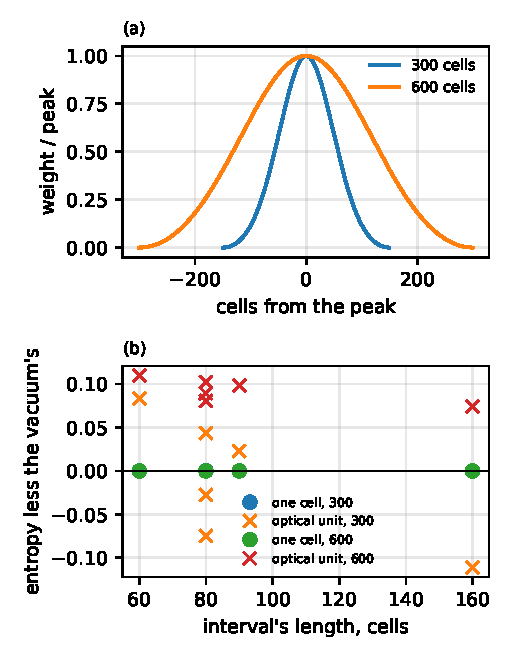
\includegraphics[width=\columnwidth]{../../build/figures/bump.pdf}
  \caption{The saddle's own weights carry the spatial reading. (a) On critical rings whose couplings vary slightly, the weights form one smooth bump around the weakest couplings, certified by the bracket. (b) The saddle state's entanglement across intervals inside the bump, against the interval's length in cells, less the vacuum's on the metric whose lapse is the weights: with one cell as the cutoff it matches, and with one unit of optical length it does not.}
  \label{fig:bump}
\end{figure}

\subsection{Where the weight vanishes}
\label{sec:readings-horizon}

Where a place falls below the common value, every reading of it stops at once. Its clock does not run, its thermometer has no finite reading, and an excitation there adds nothing to the weighted Hamiltonian's energy. Past its drop-out the simulated first cell shows all three. A static lapse vanishes at a Killing horizon~\cite{Gourgoulhon2007}, there continuously and with a finite surface gravity, here on whole places and sometimes by a jump, where no surface gravity is defined, and maximal slices of a black hole stop short of its singularity where the lapse collapses~\cite{EstabrookEtAl1973}. Read as a horizon, the weightless region is set by the energies: it sits wherever a place's density falls below the common value.

Three remarks bound this reading. A place exactly at the common value can carry no weight too, so the weight vanishes at every place below and may vanish at a place on it. And a lone weightless place keeps its links, each at half its neighbour's weight, so whether a disturbance crosses it depends on what those links do, and only a run of weightless places is a wall. Nor need deepening act as a gravitational well, since on an odd XXZ ring the deepened cell's weight, and with it its clock's rate, first rises with depth and then falls to zero (Fig.~\ref{fig:size}b).

\subsection{One value for the whole}
\label{sec:readings-whole}

The common value is the rate at which the saddle state's phase turns. Every vector $\psi^*$ in the support of the saddle state lies in the ground space of $A_{N^*}$, so
\begin{equation}
  e^{-iA_{N^*}t}\, \psi^* = e^{-ie^* t}\, \psi^* :
  \label{eq:phase}
\end{equation}
its phase turns at the common value, as the simulated state's does to the bound \val{phaseGapBound}. That phase, however, moves when a constant is added to the Hamiltonian, which the division shares equally among the places, and with the zero of the whole's clock, and no measurement inside the system sees it. So the common value as it stands cannot be the whole's own value.

% claims: critical.charge
Part of it can. At $g = J$ the transverse-field ring is critical and a problem of free fermions, so I solve uniform rings of \val{criticalSizeFirst} to \val{criticalSizeLast} cells exactly. Their common value splits into a part the same at every size, \val{criticalPerPlace} per place, which a constant added to the Hamiltonian per place moves, and a part set by the ring's size, which no such constant touches. The common value of the uniform ring is the ground energy per cell (Proposition~\ref{prop:uniform}), so the two parts are the finite-size results of conformal field theory, recovered. That part falls as one over the size squared,
\begin{equation}
  e^*(n) - e_\infty = -\frac{\pi c v}{6 n^2},
  \label{eq:casimir}
\end{equation}
with $c$ the central charge and $v$ the speed of the ring's long waves, read from its lowest levels as \val{criticalSpeed}: closing the ring at a finite size lowers the energy per cell in proportion to its waves' speed and its central charge~\cite{BloteCardyNightingale1986,Affleck1986}. Fitted, it gives $c = \val{criticalChargeSize}$, and an interval of $\ell$ cells on the largest ring gives the central charge a second way, through its entanglement entropy,
\begin{equation}
  S(\ell) = \frac{c}{3} \ln\!\Big[\frac{n}{\pi} \sin\frac{\pi \ell}{n}\Big] + \text{const},
  \label{eq:chord}
\end{equation}
which grows as the logarithm of the chord~\cite{CalabreseCardy2004}: fitted over intervals of \val{criticalShortest} to \val{criticalLongest} cells, it gives $c = \val{criticalChargeEntropy}$, the two agreeing to the bound \val{criticalChargeGapBound} (Fig.~\ref{fig:critical}).

Only the part set by the size belongs to the whole, and the reading takes that part:

\premise{constant}

The reading borrows from Henneaux and Teitelboim only that the cosmological constant is one value for the whole, conjugate to a cosmic time~\cite{HenneauxTeitelboim1989}. The size-set part falls as $1/n^2$, as $\Lambda = 3/L^2$ falls for a de Sitter horizon of growing radius $L$. Holographic dark energy likewise ties the dark energy to an infrared cut-off, the size of the event horizon~\cite{Li2004}. Its sign depends on the ring's boundary condition, for on a ring twisted across one link, whose lowest state has scaling dimension $1/8$, the critical chain's size-set part is $+\pi v/(6n^2)$ in place of $-\pi v/(12 n^2)$.

\begin{figure*}
  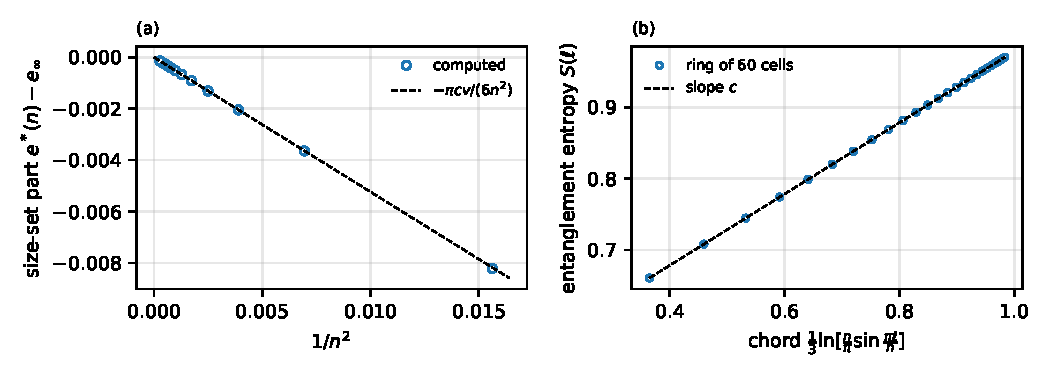
\includegraphics[width=\textwidth]{../../build/figures/critical.pdf}
  \caption{One value for the whole, on uniform critical rings. (a) The common value's size-set part falls on the conformal line, $-\pi c v/(6n^2)$, with $c = \val{criticalChargeSize}$. (b) An interval's entanglement entropy on the ring of \val{criticalSizeLast} cells rises along the chord with slope $c = \val{criticalChargeEntropy}$, the same central charge read a second way.}
  \label{fig:critical}
\end{figure*}

\subsection{A part's horizon and its temperature}
\label{sec:readings-patch}

A part of a system has a horizon too, at the edges where the weights of its entanglement Hamiltonian, defined below, vanish. Comparing a part's weights with the saddle's takes a premise:

\premise{subsystem}

I take an interval of $\ell$ cells of the infinite critical transverse-field chain and compute its entanglement Hamiltonian from the chain's correlations~\cite{Peschel2003}, in Majorana operators, $K = \tfrac{i}{4}\sum_{ab} k_{ab}\gamma_a\gamma_b$ with the interval's state proportional to $e^{-K}$, where $\gamma_{2p}$ and $\gamma_{2p+1}$ belong to cell $p$, $\gamma_a^2 = 1$, and the chain's ground state has $\langle i\gamma_{2p}\gamma_{2q+1}\rangle = -2/\big(\pi(2q - 2p + 1)\big)$, which fixes their signs. The correlation matrix's eigenvalues bunch near $\pm 1$, so the computation runs in multiple-precision arithmetic. The interval's weights are the coefficients of $K$ set against the chain's terms, each placed where its term sits. A term of range $m$ adds $m$ times its coefficient to a long wave's energy, so the weight at bond $a$ counts the longer-range terms with that factor,
\begin{equation}
  \beta_a = \frac{1}{2J}\sum_{m\ \mathrm{odd}} m\, k_{b,\,b+m}, \qquad b = a - \tfrac{m-1}{2}:
  \label{eq:moment}
\end{equation}
each odd-range coefficient centred on the bond, weighted by its range. The conformal profile emerges in the same way on free-fermion hopping chains, once the hopping to distant neighbours is counted~\cite{EislerTonniPeschel2019}, and across lattice models whose low-energy theory is Lorentz invariant the Bisognano--Wichmann form describes the entanglement Hamiltonian accurately~\cite{GiudiciEtAl2018}. Here it is read on the critical transverse-field chain.

% claims: patch.profile
The weights take the profile of a horizon. For intervals of \val{patchLengthFirst} to \val{patchLengthLast} cells, read with their longer-range terms, they follow
\begin{equation}
  \beta(x) = \frac{2\pi}{v}\,\frac{x(\ell - x)}{\ell},
  \label{eq:patch}
\end{equation}
to the bound \val{patchShapeBound} of their largest at the longest, with coefficient \val{patchCoefficient} against $2\pi/v = \val{patchTwoPi}$ (Fig.~\ref{fig:patch}). The weight is zero at both edges, largest in the middle, and rises from each edge with slope $2\pi/v$: the profile of an interval's modular Hamiltonian in a conformal field theory~\cite{CasiniHuertaMyers2011}, and of the wedge Bisognano and Wichmann describe~\cite{BisognanoWichmann1976}. Read from the nearest terms only, the coefficient is \val{patchNearCoefficient}, and the profile's shape departs from $x(\ell - x)/\ell$ by about \val{patchNearShape} of its largest, and the longer-range terms carry the rest.

\begin{figure*}
  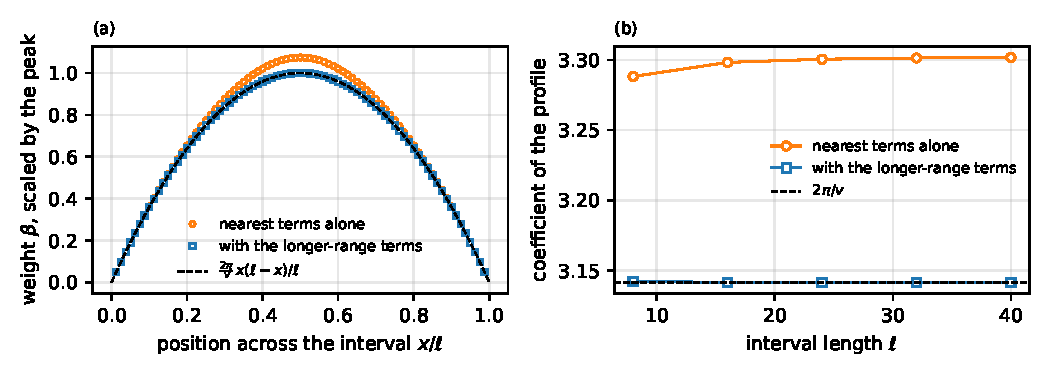
\includegraphics[width=\textwidth]{../../build/figures/patch.pdf}
  \caption{A part's horizon. (a) The weights of an interval's entanglement Hamiltonian on the critical chain, scaled by the peak of the weights read with their longer-range terms: read with their longer-range terms they lie on $x(\ell - x)/\ell$ with coefficient $2\pi/v$, and from the nearest terms only their coefficient is larger and their shape departs from the curve by about \val{patchNearShape} of their largest. (b) The coefficient against the interval's length: with the longer-range terms it settles on $2\pi/v$, and from the nearest terms alone at \val{patchNearCoefficient}.}
  \label{fig:patch}
\end{figure*}

Each edge, read as a horizon, has a temperature under the premise on light cones (Sec.~\ref{sec:readings-space}). Scaled to one at the interval's centre, the weights fall to zero at each edge with slope $4/\ell$ per cell, and that slope is a surface gravity $\kappa$ because every cell has the same proper length (Sec.~\ref{sec:readings-space}). The temperature it gives, $v\kappa/2\pi$, equals the local temperature at the centre exactly when the coefficient is $2\pi/v$, as Tolman's relation across a static patch requires. So the ratio of the two temperatures is the coefficient over $2\pi/v$, and the reading adds an identification to the profile, not a further number. Read with the longer-range terms, the ratio of the two temperatures differs from one by \val{patchRatioGapFirst} at the shortest interval to \val{patchRatioGapLast} at the longest, and from the nearest terms it is \val{patchNearRatio}.

A part's horizon is not the saddle's. A part's weights vanish at its edges with a finite slope, while the saddle leaves a weightless place at zero outright, so the two share the vanishing and not the slope. Nor are a part's weights the saddle weights of the part taken alone, which for the open chain sit at its two ends.

Read as the cosmological horizon, a part's horizon has a known temperature:

\premise{patch}

The temperature is then Gibbons and Hawking's~\cite{GibbonsHawking1977},
\begin{equation}
  T_{\mathrm{dS}} = \frac{\hbar c}{2\pi k_B}\sqrt{\frac{\Lambda}{3}} = \frac{\hbar H_0 \sqrt{\Omega_\Lambda}}{2\pi k_B},
  \label{eq:desitter}
\end{equation}
with $c$ here the speed of light and $\Lambda = 3\Omega_\Lambda H_0^2/c^2$: the horizon's surface gravity over $2\pi$, from the measured expansion. With the Hubble rate \val{planckHubble}~km/s/Mpc and dark-energy fraction \val{planckFraction}~\cite{Planck2018}, it is \val{desitterTemperature}, with the \val{desitterSpread} uncertainty those values carry. Local determinations of the Hubble rate differ from Planck's, and the temperature scales with the rate. The system supplies only the $2\pi$, the Bisognano--Wichmann coefficient; the measured rate and Gibbons and Hawking's formula are input. The rate $H_0\sqrt{\Omega_\Lambda}$ is the expansion's asymptotic de Sitter rate, not that of the present event horizon.

\subsection{Chance from records inside}
\label{sec:readings-records}

Chance comes to a part the way time does, through conditioning, here on records:

\premise{records}

The premise restricts what Bong and coauthors call the absoluteness of observed events~\cite{BongEtAl2020} to readings copied outside their place. It is close to the objectivity that redundant records in an environment confer, since only states that leave many copies can be found out by many observers, who then agree~\cite{OllivierPoulinZurek2004,Zurek2009}. Bell's theorem limits what such chance can be: the frequencies two separated parts read cannot all come from one description that fixes every reading's outcome together, each part's by its own setting~\cite{Bell1964}. The limit is a bound on
\begin{equation}
  S = E(0,0) + E(0,1) + E(1,0) - E(1,1),
  \label{eq:chsh}
\end{equation}
where $E(x,y)$ is the correlation of a reading with setting $x$ on one part and a reading with setting $y$ on the other~\cite{ClauserEtAl1969,Tsirelson1980}: in words, three correlations less the fourth.

% claims: bell.factorization
The bound factors into two assumptions. For two readings on each of two parts, self-adjoint with square one, $S$ is at most \val{bellLocal} when all four readings commute, and at most $2\sqrt 2$ when only readings of different parts commute (Proposition~\ref{prop:factorization}), the second Tsirelson's bound~\cite{Tsirelson1980}. Both bounds assume that readings of different parts commute, so the whole gap between them is whether a part's two readings commute. On a maximally entangled pair, the readings that reach \val{bellQuantum} commute between the parts and not within one.

% claims: records.gluing
Whether a part's frequencies glue into one description is a linear program, a largest share over joint descriptions~\cite{Fine1982,AbramskyBrandenburger2011}, and like the saddle's programs it has a dual and a witness either way~\cite{AbramskyBarbosaMansfield2017}: the joint description, or the inequality it breaks. For the readings that reach $2\sqrt 2$ on a maximally entangled pair, the largest share of their frequencies one description carries is \val{gluingShare}, by a linear program and by its dual to the bound \val{gluingDualBound}, leaving \val{gluingContextual} that cannot glue~\cite{AbramskyBarbosaMansfield2017}. The dual's weights are the CHSH inequality.

% claims: history.conditioning
To hold the protocol of chance inside it, a whole must hold a sequence of steps at once. For unitary steps $U_1, \dots, U_T$ applied to a starting state $\psi_0$, with a register counting the steps, the history Hamiltonian~\cite{Feynman1986,KitaevShenVyalyi2002}, here with a start term that fixes the whole starting state, is
\begin{equation}
\begin{split}
  H = {} & |0\rangle\langle 0| \otimes \big(I - |\psi_0\rangle\langle\psi_0|\big) \\
  & + \sum_{t=1}^{T} \tfrac12\big(|t\rangle\langle t| + |t{-}1\rangle\langle t{-}1|\big) \otimes I \\
  & - \sum_{t=1}^{T} \tfrac12\big(|t\rangle\langle t{-}1| \otimes U_t + \mathrm{h.c.}\big) .
\end{split}
  \label{eq:history}
\end{equation}
In words, it penalizes a start other than $\psi_0$ and links each reading of the register to the next through that step. It is positive semidefinite, its null space is spanned by the state that holds every step at once, and conditioned on the register's reading $t$ the rest is the state after $t$ steps (Proposition~\ref{prop:history}). This is analogous to the conditioning of Proposition~\ref{prop:conditioned}, with a clock whose readings are the steps.

A protocol puts the readings inside the whole. Two friends, Charlie and Debbie, each measure half of a maximally entangled pair and record the outcome, and each record is copied outside its place, the copy's two states overlapping by $\gamma$: one for no copy, zero for a full one. Alice either reads Charlie's record or measures his laboratory as Wigner may, here by reversing his measurement and reading his qubit in another basis, and Bob does the same with Debbie's~\cite{Brukner2018}. Here their settings are held in qubits, and Appendix~\ref{app:models} gives every step. I hold the protocol as the null state of its history Hamiltonian, Eq.~\eqref{eq:history}, over \val{recordsQubits} qubits and \val{recordsSteps} steps, solved once: its least energy is below the bound \val{recordsEnergyBound}, and its gap is \val{recordsHistoryGap}, which depends only on the number of steps, since the rotation in the proof of Proposition~\ref{prop:history} carries every protocol's history Hamiltonian to that of the protocol that does nothing.

% claims: records.chsh
The violation follows the copy. Conditioned on the register's last step, Alice's and Bob's outcomes give
\begin{equation*}
  S = \frac{(1 + \gamma)^2}{\sqrt 2}
\end{equation*}
to the bound \val{recordsGapBound} at every overlap computed, from \val{recordsChshFirst} with no copy to \val{recordsChshLast} with a full one (Fig.~\ref{fig:records}): the correlations weaken as the copy strengthens. A direct calculation gives the same, $E(0,0) = 1/\sqrt 2$, $E(0,1) = E(1,0) = \gamma/\sqrt 2$ and $E(1,1) = -\gamma^2/\sqrt 2$, and the whole solved once reproduces it. They exceed the bound \val{bellLocal} of one description of absolute outcomes, the local-friendliness bound, which with two settings on each side is Bell's~\cite{BongEtAl2020}, only while the overlap exceeds \val{recordsThreshold}, and no reading on one side moves with the other side's setting by more than the bound \val{recordsSignalBound}. The threshold belongs to these settings, not to the copy. With both friends reading $Z$ and the second settings turned from $Z$ toward $X$ by $\theta$ on Alice's side and $-\theta$ on Bob's, the same steps give $S = 1 + 2\cos\theta - \cos^2\theta + \gamma^2\sin^2\theta$, whose largest value, at $\cos\theta = 1/(1 + \gamma^2)$, is $2 + \gamma^4/(1 + \gamma^2)$: above the bound at every overlap short of a full copy. Only a full copy, $\gamma = 0$, keeps every setting within it.

Read under the records premise, what a part reads as chance is which record its description is conditioned on. Nothing is drawn in the whole's frame, since the stationary whole holds every reading together, and the readings can be correlated beyond one description of absolute outcomes only while no copy of them outside their places is full; with the settings computed, only while any copy is weaker than their threshold.

\begin{figure}
  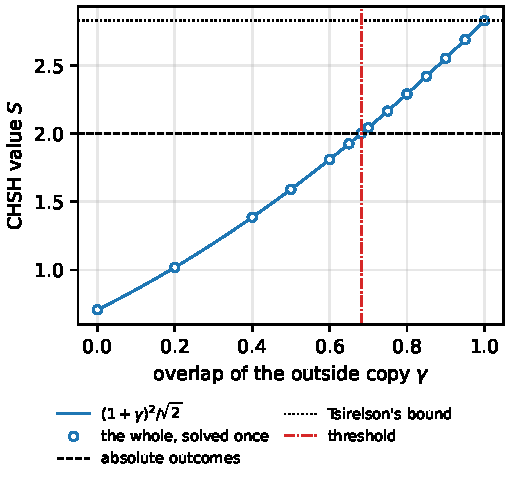
\includegraphics[width=\columnwidth]{../../build/figures/records.pdf}
  \caption{Chance from records inside. The CHSH value of Alice's and Bob's outcomes, conditioned on the last step of the whole solved once, against the overlap of the outside copy of their records: on $(1+\gamma)^2/\sqrt 2$, above the bound of one description of absolute outcomes (dashed) only while the copy is weaker than these settings' threshold (dash-dotted), and below it once the copy is stronger than that.}
  \label{fig:records}
\end{figure}

\begin{table*}[tp]
  \caption{The paper's one dataset, a published entanglement profile, set beside the readings rather than used to test the claims.}
  \label{tab:datasets}
  \footnotesize
  % GENERATED from src/saddle/tables.py by `make generate`; edit the source, not this file.
\begin{tabular}{p{2.7in}lp{2.1in}l}
\toprule
\raggedright Data & Role & \raggedright Bears on & Standing \tabularnewline
\midrule
\raggedright Measured entanglement-Hamiltonian weights of a subsystem at the end of a 51-ion chain, bond by bond~\cite{JoshiEtAl2023} & correspondence & \raggedright Tolman temperature, horizon & fixed by comparison \tabularnewline
\bottomrule
\end{tabular}

\end{table*}

\section{A measured entanglement profile}
\label{sec:data}

One published measurement can be set beside the readings, though it cannot test the claims, which concern the saddle of a known Hamiltonian. An entanglement Hamiltonian learned from measurements of a part~\cite{KokailEtAl2021} is fitted in the form of the part's state of greatest entropy given its measured local terms,
\begin{equation}
  \rho_A = \frac{1}{Z}\exp\Big(-\sum_k \beta_k h_k\Big), \qquad \operatorname{Tr}(\rho_A h_k) = m_k ,
  \label{eq:entanglement}
\end{equation}
with $h_k$ the local terms, $m_k$ their measured values and $\beta_k$ the multipliers, the weights a part's measurements put on its local energies. Under the premise on subsystems (Premise~\ref{premise:subsystem}) these are weights of the saddle's kind.

Joshi and coauthors measured such a profile on a chain of trapped ions~\cite{JoshiEtAl2023} (Table~\ref{tab:datasets}). They prepared ground states of the Heisenberg XXZ chain with open ends, its form engineered from XY interactions of controllable range, and learned the entanglement Hamiltonian of a subsystem as the chain's terms weighted by place. The profile held here is the ground state's at the isotropic point, bounded by a cut. The weights are the learned inverse temperatures on the bond terms, with their published standard errors. Its weights, inverse temperatures in units of the inverse of the chain's coupling, taken from the published archive without its row at the cut itself, which the archive gives as zero with no error, rise by \val{profileSlope} per site moving away from the cut and extrapolate at the cut to \val{profileCutFraction} of their largest. The term nearest the cut holds \val{profileNearRatio} of the largest, so the inverse weight, the local temperature, peaks at the cut. Farther from the cut the weights reach a largest value and fall again toward the chain's last site, where the shape of a weight vanishing at an edge no longer holds.

A comparison with the claims would need more: each local term of a known Hamiltonian measured place by place with its standard error, on a system whose saddle can be computed, so that a measured largest density could be set against the computed common value. Since the bound is a theorem, such a comparison would test the measurement and its calibration rather than the claims, and what data can bear on are the readings. Variational eigensolver runs sample every term of small known Hamiltonians~\cite{KandalaEtAl2017} but report only totals, not the terms place by place.

\section{Limits}
\label{sec:limits}

\begin{enumerate}
\item The programs over states run on small systems: the ring of \val{ringCells} qubits with one deepened cell, the open chain of \val{exitChainCells} cells, the catalogue up to \val{catalogueLargest} cells and the study of size up to \val{scalingLargest} cells; the closed-form Ising depths reach \val{depthsLargest} cells by the full Hamiltonian. Free fermions reach further, on transverse-field chains only: the Ising depths to \val{largeLargest} cells, the critical rings to \val{criticalSizeLast}, the bumps to \val{bumpSweepCellsMost} and the spatial readings' chain of \val{spaceCells}. The derived statements hold at every size; the computed ones hold where they are computed.
\item The optimal weighting is shown unique by Proposition~\ref{prop:single} on the six-cell Ising ring before its drop-out, the weights the simulations read, and past it within the deepened spin's sector, and in \val{uniqueCertified} of the catalogue's \val{uniqueModels} cases, each model before and after deepening; in \val{uniqueNarrow} other models it is bounded only to a width, and in \val{uniqueWide} it spreads wider, a set wherever two places each hold the common value alone. Every split of the weight between the open chain's two ends is optimal, and its signals of Sec.~\ref{sec:readings-space} are computed at the even split, the coldest equilibrium's limit there. With the field off, the four-cell XXZ ring's other cells have no unique optimal weighting at all. Elsewhere a computation takes the solver's weighting.
\item The state-side drop-out depths are computed to a tolerance on the other cells' common value and come in low, because near the depth, where the weight falls continuously to zero as on the Ising ring, the full common value approaches that value only quadratically, so a tolerance on the value becomes an error of the order of its square root in the depth. The closed-form Ising depths are free of it. The Ising depth's limit comes from a fit, and how the depth depends on the coupling is not studied.
\item The printed catalogue is the narrower of two; the wider one, at the same small sizes, with larger rings in the study of size, is stored with the code. In it every computed pair meets every general claim, except that on one XXZ ring the two programs' values differ by more than the bound \val{catalogueGapBound}, its solver having stopped short of its tolerances: there the computation fell short, not a claim.
\item The readings rest on their premises, which are stated and not derived; the premise of evolution takes the weighted Hamiltonian, not the Hamiltonian, as what generates the time a part reads, and every reading of time rests on it. The simulations compute each reading's quantity under its premises and do not test them. The probes read as test probes. Lemma~\ref{lem:probes} counts their ground energy, and an excited probe adds its excitation to its place's density and can move the saddle, so the readings take the excitation small.
\item The weights depend on how the system is cut into places. Grouping the ring's cells in pairs, whose canonical densities are the cells' sums, changes the common value and the weights; past the drop-out the pair holding the deep cell carries no weight, while the cell inside it beside the deep one carries some.
\item The spatial reading is a chain's, and a one-dimensional spatial metric has no curvature, so on a chain the reading's whole content is that every cell has the same length; on more dimensions it gives a metric only if long waves move at one speed in every direction, which is not tested here. As a weak field, a lapse over flat cells bends light half as much as general relativity does: in post-Newtonian terms $\gamma_{\mathrm{PPN}} = 0$, where radio links with the Cassini spacecraft measured $\gamma_{\mathrm{PPN}} = 1$~\cite{BertottiIessTortora2003}. A continuum geometry meets the reading only at a resolution, as a sharp step's share of a turned-back wave shows. And the saddle's smooth weights come as a bump whose width grows about as $(n^2/\epsilon)^{1/4}$ on the \val{bumpFitCount} rings computed where the variation is large against the uniform floor's curvature, and spans about half the ring on the others, which describes those rings rather than a rule; the deepened rings, with their longitudinal field, are not free fermions and lie outside that computation.
\item The weights are sensitive where the floor is flat. Around uniform weights on a uniform critical ring the floor's flattest curvature, for a unit change of the weights, falls with the size, roughly as $n^{-\val{bumpFlatPower}}$ between \val{bumpCellsFirst} and \val{bumpCellsLast} cells, so couplings varied by a small fraction move the weights by order one, and at a fixed variation the share of the ring with appreciable weight shrinks as the ring grows. A reading of the weights as a lapse inherits that sensitivity. Whether the optimal weighting has a limit as the size grows is not studied.
\item The programs run over the full space of states, so their cost grows exponentially with the number of places, and checking a weighting's floor is a ground-energy problem, hard in general: deciding whether a two-local Hamiltonian's ground energy lies below one bound or above another, an inverse polynomial higher, is complete for QMA, the quantum analog of NP~\cite{KempeKitaevRegev2006}.
\item Nothing here says which of Bell's assumptions fails beyond where the whole's frame places the failure, and the threshold \val{recordsThreshold} belongs to this inequality and these settings, since turned settings cross the bound at every overlap short of a full copy: crossing the bound refutes absolute outcomes, local agency and independent settings together, and the whole's frame, keeping the other two, reads it as a reading that is not absolute, while staying under it shows nothing.
\item The division is the one open definition: each own piece to its place, and split each link's piece equally. Proposition~\ref{prop:unique} shows it is the only division meeting its requirements. Whether a closed system forces those requirements is open. The division needs a space of finite dimension at each place, whose maximally mixed state fixes each zero, and for oscillators or fields it does not exist as defined. Those zeros also decide, of two systems that do not interact, which takes all the weight, so adding a decoupled system can stop every clock in the other: read as a lapse, the weights do not separate into clusters. The weights, the drop-out depths and the open chain's weight at its ends all depend on it; the saddle's general propositions hold for any densities that sum to the Hamiltonian.
\item Seven derived statements are proved here and not in Lean: the canonical division, its uniqueness, the history construction, the coldest equilibrium and its symmetric limit, the parity of rings, and the single optimal weighting. Their proofs need partial traces over many places, Schur's lemma for products of unitary groups, an operator identity on a register and a rest, maximum-entropy duality for density matrices, and perturbation theory of a ground state, which Mathlib does not yet state. The repository's Lean project proves the other derived statements against Mathlib, each named beside its proposition in the repository's blueprint, two of them in part: the bracket's closing remark, that the conditions need not certify a pair otherwise, and the first clause of Corollary~\ref{cor:crossing}, which follows at once from Eq.~\eqref{eq:evolution}, are proved here only. The factorization of Bell's bound is checked as Mathlib's two theorems for ordered star-algebras, stated in the paper's terms; their instantiation on matrices is left.
\end{enumerate}

\section{Certificate, price and clock rate}
\label{sec:composition}

The proofs and computations above stand without this section.

I take the results to be one object seen whole where it is usually seen in pieces. The same weights certify how low every place's energy can be held, price each place's bound, and set the rate at which each place's clock runs. The theorem fixes them, the computations show them at work, the readings say what they are under stated premises, and the data set a measured profile of the same kind beside them. A reader from many-body physics meets them first as a certificate, a reader from gravity first as a lapse, and the paper is arranged so that each finds the other's object to be the same one. That they coincide is, for me, the content of the result. That they form a lapse is how I read it.

I undertook the work to learn whether a closed system's local energies, with no clock outside it, fix the rates at which its places run. They fix the weights, through the saddle, and the rest of this section reads what those weights are.

\emph{What the object is for.} I offer the saddle not as a theory of the whole but as a way to reach one. The way is to seek the object that the descriptions physics already uses are limits of, rather than one more description beneath them. The saddle is an object of that kind: every state of the system meets its bound, and known descriptions come back from it under stated premises, as limits where they are limits, each holding where its premise and its limit hold. For static descriptions the paper's readings go that far, and under its premises they recover \matchedreadings. Most of these hold for any weighting; the saddle supplies which weighting, where it vanishes, and that its weights are prices. Each is known, and that is the point: a known description reached from a different object, under a stated premise, shows what the object can carry. Whether it carries the rest is the work ahead, and Sec.~\ref{sec:limits} says where the present work stops.

\emph{The saddle.} The saddle is a bottleneck. Over all its states a system realizes a convex set of local-energy profiles, one number per place. The common value is the lowest level some realizable profile stays at or below everywhere, and the weights are the tilt of the plane that supports the set there~\cite{BoydVandenberghe2004}. The same structure is the value of a two-player game~\cite{vonNeumann1928}, a system of prices in which each multiplier is what relaxing its bound is worth~\cite{Kantorovich1960}, and the least achievable largest load when work is spread across machines. Its nearest relative in many-body physics, the lower bound assembled from the least energies of local pieces~\cite{Anderson1951}, answers a different question. I read the common value as a property of the places together, not of any one of them, and the weights as the record of where the whole is tight: a place with weight is part of the bottleneck, and lowering a place without weight leaves the common value where it is. Its first use is in measurement. Any experiment that measures every local term of a known Hamiltonian, place by place, has a hard family of inequalities to meet: for every weighting, the weighted average of its numbers stays at or above that weighting's floor. A violation means its numbers belong to no state of the operators it names, and the weights say where a prepared state's excess above the floor sits. It also governs edges, at least in the model studied: on the open transverse-field chain the two ends hold the floor up, each able to hold it alone, so lowering an interior place's energy changes nothing, nor does lowering one end, while lowering both ends lowers the common value. Whether the open devices experiments use behave the same way is not established here. If they do, it is the most practical consequence, since open boundaries are the rule. The usual Hamiltonian is exactly the uniform weighting scaled by the number of places, which is algebra, and the gain of reweighting, Eq.~\eqref{eq:gain}, is what keeping that weighting costs in the common value. On a uniform ring the cost is zero and the usual model loses nothing; elsewhere the saddle says what the uniform weighting costs.

\emph{The weights as a lapse.} In canonical gravity the lapse is the rate at which proper time advances along the normal to a slice, and it is chosen with the slicing~\cite{Gourgoulhon2007}. In a static spacetime it is not a choice: the slicing adapted to the static time fixes it as the redshift factor, and Tolman's relation holds with it~\cite{Tolman1930}. That is the lapse I take the weights to be. It is not a gauge condition for dynamical slicings, but what a static lapse becomes when a system has no geometry to read it from, only local energies. The canonical division, with the saddle, fixes the weights as the static slicing fixes that lapse (Sec.~\ref{sec:division}), and the readings that match Tolman's relation and the redshift are the identification at work (Sec.~\ref{sec:readings}). Devices that already weight local terms by place meet it directly. Entanglement Hamiltonians are realized with couplings that vary in space~\cite{DalmonteVermerschZoller2018}, and the sine-square deformation weights an open chain so that its ground state becomes a ring's~\cite{HikiharaNishino2011}. Each of those weightings is chosen for a purpose. The saddle's is fixed by the energies, and on the open chain studied it is the opposite of the sine-square profile, all its weight at the ends where that deformation puts none, because it answers a different question. The contrast is the open chain's: on the two critical rings computed whose couplings vary least against the uniform floor's flattest curvature, the saddle's bump spans about half the ring, as the sine-square profile does, following the one wave the variation imposes. In its own frame the whole has no clock. It is stationary, and it holds every reading of every clock inside it at once, so what a part calls past and future are both in it; time is read only between parts, by conditioning on a clock among them (Sec.~\ref{sec:frame}). Nor are the places the whole's own, since like the clock they belong to a description. They are taken as given here, one qubit to a cell, and the saddle is a condition the whole satisfies at that resolution, its weights changing with the cut (Sec.~\ref{sec:limits}). What the whole does fix is the frame it sets its parts, the relative rates at which their clocks run, and those rates are the weights. Where the places are alike that frame is uniform: every clock runs at one rate, a single cosmic time, which is what the parts read there and not a clock the whole keeps. The usual Hamiltonian takes that uniform frame everywhere. Its use, as I read it, takes without saying so the frame of one clock outside the system, and the gain of reweighting is what that frame costs against the one the whole sets its parts.

\emph{The stopped clock.} A place so deep that the others, optimized without it, already hold it at or below their common value carries no weight, and its clock stops. A static lapse vanishes at a horizon. Maximal slicing collapses the lapse too, but that zero belongs to a chosen slicing~\cite{EstabrookEtAl1973}. I read the drop-out as a horizon's structure arising from the energies alone, a zero no slicing chose. The coldest equilibrium reaches the weights only as its bound reaches the floor, so I also read the drop-out as the cold limit of a lapse profile, sharp only there. In practice a strongly detuned or pinned site stops constraining the rest once it is past its drop-out depth. Where the couplings conserve the magnetization, an even ring keeps it under a weak field; on an odd ring the outcome follows from the other places' optimal states, and on one of the rings studied they turn its spin against its field and keep it as well.

\emph{Selection.} A reader may ask what selects this optimum, or why nature would. The question supposes that something chooses among states, and in this frame nothing does. The energies have the optimum as they have a lowest eigenvalue: the floor and the weights belong to them whether or not any state sits there, and Eq.~\eqref{eq:certificate} bounds every state alike. The paper states the optimum in three ways, none with an agent. As a pair, the weighted Hamiltonian holds the state at its lowest eigenvalue while weight sits only where the state's densities reach the common value, each optimal against the other (Eq.~\eqref{eq:conditions}). As geometry, the weights are the normal of the plane that supports the realizable energy profiles at the common value (Sec.~\ref{sec:saddle}). And where the optimum is unique, they are the shape of the coldest equilibrium a common bound on every local energy allows (Proposition~\ref{prop:coldest}). Only the premise of evolution puts the system at its floor, and it is a condition too (Sec.~\ref{sec:frame}). An optimum met is no more chosen than a light ray chooses the path along which its travel time is stationary. Where the optimum is a set, as on the open chain, nothing narrows it: the energies fix the set, and a computation that needs one weighting takes one and says which. Two questions stay open, one of dynamics and one of limits: whether a system prepared in another state relaxes toward the saddle, and whether, where the optimum is a set that no symmetry narrows to one point, the coldest equilibrium's proportions converge to one of its points; on the open chain its reflection makes them tend to the even split.

\emph{The spatial part.} The readings give both parts of a static geometry (Sec.~\ref{sec:readings}). Its time part is the frame the whole sets its parts. Its spatial part is the description's: long waves cross every cell in the same time, read by the clock at the cell, so every cell has the same proper length whatever its weight, and the whole adds only the lapse (Sec.~\ref{sec:readings-space}). Distances read in the whole's time stretch where the weights are small and diverge where they vanish, as the time to reach a horizon does; distances summed cell by cell do not. The description's cells are alike in space, and the whole makes them unlike in time. The saddle state carries the same geometry with no clock: its entanglement fixes its weights as the lapse. This is not general relativity's geometry, whose static fields curve space as well as time, and it is not offered as one.

\emph{Chance.} The same frame offers a reading of chance. Nothing in the whole is drawn or chosen, and the evolution a part reads is generated by a sum of local terms. What a part reads as chance is which record its description is conditioned on, in shares the state of the whole fixes. Stochasticity, on this reading, is a part's relation to its records rather than a property of the whole. The reading of chance from records shows where this frame places the failure of Bell's assumptions: on a reading being the same for every description before a copy of it exists outside its place, a premise stated with the reading, while the computation shows the violation fading as the copy is made (Sec.~\ref{sec:readings-records}). A reader who takes every outcome as absolute reads Bell's theorem as refuting locality instead, and that disagreement is with the premise, not with the computation.

\emph{Toward a theory of the whole.} For a closed universe the absences above are total: no clock outside, no places but a description's, nothing drawn. The object, stated like everything here in quantum theory's terms, is then a candidate condition for a theory of the whole. The canonical formalism multiplies the local Hamiltonian constraints by a lapse it leaves free~\cite{ArnowittDeserMisner2008}. Quantizing the constraints and imposing each sharply, as canonical approaches do, meets their algebra, which closes only with functions on phase space for its coefficients; the master constraint replaces them by one condition that holds exactly where all of them do~\cite{Thiemann2006}. The saddle asks for something that, for finitely many places, always exists: the largest local energy held as low as it can be. Its multipliers are fixed by optimality rather than left free. One weighted constraint holds exactly, since an optimal state is a ground state of the weighted Hamiltonian at the common value, and the local constraints hold where they bind. The part of the common value the whole's size sets reads, for me, as one constant for the whole, the role a cosmological constant plays in Henneaux and Teitelboim's reading~\cite{HenneauxTeitelboim1989}, conjugate here to a clock's reading inside the whole rather than to a time the whole keeps; on the rings computed, its sign depends on how the ring is closed. The object constrains such a theory as well: no state of the whole holds every local energy below the common value, and only places that reach it carry weight. Two things stand between this and a theory of the whole. The theorem ranges over mixed states. Where the weighted Hamiltonian's lowest level is a single state, the optimal state is that state, and pure (Proposition~\ref{prop:conditions}); where the level is degenerate, a pure state need not reach the same floor: on one qubit whose six places hold $\pm X$, $\pm Y$ and $\pm Z$ the common value is zero, which no pure state reaches. Where the pieces are real, as in every model here, and the level is a pair, a pure state of the pair holds every density where the optimal state does, so one reaches it; with complex pieces, as the qubit shows, or with a level of three states, as on a qutrit whose ten places hold plus and minus each of the five real Gell-Mann matrices, a pure state need not, and whether one does in a given model is open. And it needs finitely many places, each with finitely many levels, so a continuum theory meets it only at a resolution.

\section{Conclusion}
\label{sec:conclusion}

A closed quantum system holds its local energies down to one common value. The weights vanish wherever a place falls short; a deepened place drops out exactly when the other places, optimized without it, already hold it at their value; and on an even ring that conserves the magnetization, under Proposition~\ref{prop:parity}'s hypotheses and to first order in a small field, it never does, while on odd rings the outcome follows from the other places' optimal states. Under the premise of evolution, a whole stationary under the weighted generator with a clock among its parts, the weights are the clock rates and redshifts of a static lapse, and under the premise of equilibrium its inverse temperatures. So one weighting certifies how low every local energy can be held and names the places that hold it up, and the same weighting is a lapse that the energies, once divided among the places, fix by themselves, zero wherever a place falls short.

\textit{Data and code availability.} Everything behind the paper is public at \url{https://github.com/davidtswanson903/minimax-lapse}: the code, the Lean proofs, and the results every printed number is read from, which one command regenerates.

\textit{Origin.} The result first arose in separate work. It is restated and checked here independently, and rests on nothing from there.

Beside the questions the sections before leave open, three more stay open: whether the Ising drop-out depth, \val{largeDepthLast} at \val{largeLargest} cells and fitted to \val{largeLimitLate}, has a closed form on the infinite ring; whether, beyond the XXZ family, a conservation law keeps a deepened place's weight as the magnetization does on even rings; and whether the weights still read as a lapse away from equilibrium, where static spacetimes give no guide.

\appendix

\section{The canonical division}
\label{app:division}

One division of the energy names no place. Write $E_T(H) = \operatorname{tr}_{X\setminus T}(H)/d_{X\setminus T} \otimes I_{X\setminus T}$ for $H$ averaged over every place outside a set $T$.

\begin{proposition}\label{prop:canonical}
Every operator $H$ on finitely many places splits in exactly one way as $H = \sum_{S} H_S$ over the sets $S$ of places, with $H_S$ acting on $S$ alone and averaging to zero over each place of $S$; the parts are
\begin{equation}
  H_S = \sum_{T \subseteq S} (-1)^{|S \setminus T|}\, E_T(H).
  \label{eq:canonical}
\end{equation}
Sharing each part equally among the places of $S$, and the constant part $H_\emptyset$ among all places, gives densities that sum to $H$; when every piece of a model acts on its places and averages to zero over each of them, as every model here does, these are its densities.
\end{proposition}
\begin{proof}
Each $E_T(H)$ acts on $T$, so $H_S$ acts on $S$, and $\sum_S H_S = E_X(H) = H$ by Möbius inversion over the subsets of $X$. Averaging $H_S$ over a place $x \in S$ maps $E_T(H)$ to $E_{T\setminus\{x\}}(H)$, so the terms for $T$ and $T \cup \{x\}$, of opposite sign, cancel in pairs and the average is zero. If $\sum_S G_S = 0$ with each $G_S$ of that kind, then $E_T(G_S) = G_S$ for $S \subseteq T$ and $E_T(G_S) = 0$ otherwise, since $S$ then has a place outside $T$ over which $G_S$ averages to zero; so $\sum_{S \subseteq T} G_S = 0$ for every $T$, and by induction on the size of $T$ every $G_S$ is zero. A piece that acts on its places and averages to zero over each is its own part, so a model built from such pieces, each own piece given to its place and each link's piece split equally between its two ends, has the canonical densities.
\end{proof}
For qubits the part on $S$ is the sum of the terms of $H$ that are Pauli strings acting on exactly the places of $S$.

The canonical division is the only one meeting four asks a division can be held to.

\begin{proposition}\label{prop:unique}
Let a division give each Hamiltonian $H$ on the places densities $D_x(H)$ that sum to $H$. If it is linear in $H$; covariant under a change of basis at any place, $D_x(UHU^\dagger) = U D_x(H) U^\dagger$ for every $U = \bigotimes_y U_y$; gives each part $H_S$ of Proposition~\ref{prop:canonical} with $S$ nonempty only to the places of $S$; and shares each part alike among its places, and the constant part alike among all places; then it is the canonical division.
\end{proposition}
\begin{proof}
The operators split as the direct sum over sets $S$ of the spaces $V_S$ of parts acting on $S$ and averaging to zero over each of its places, $V_S = \bigotimes_{y \in S} \mathfrak{sl}_y$ with $\mathfrak{sl}_y$ the traceless operators at $y$. Conjugation by $U_y$ acts on $\mathfrak{sl}_y$ irreducibly, so $V_S$ is irreducible under the product of the groups, and no two $V_S$ are equivalent, since they differ in the places whose group acts. A real-linear map commuting with every change of basis extends to the complexified spaces, on which each $V_S$ stays irreducible and no two are equivalent, so by Schur's lemma it multiplies each $V_S$ by a number, real because the map keeps operators Hermitian: $D_x(H) = \sum_S a_x(S)\, H_S$. Giving each part with $S$ nonempty only to its places makes $a_x(S) = 0$ for $x \notin S$, summing to $H$ makes $\sum_x a_x(S) = 1$, and sharing alike makes $a_x(S) = 1/|S|$ for $x \in S$ and $a_x(\emptyset) = 1/|X|$: the canonical densities. Putting each part's zero at its lowest level is not linear, since the lowest level of a sum is not the sum of the lowest levels, and the shifts of Proposition~\ref{prop:division} add constants that are not linear in $H$, since they depend on it through a ground state.
\end{proof}
Without the last requirement the division is any $D_x(H) = \sum_S a_x(S)\, H_S$ with $a_x(S) = 0$ off $S$ and $\sum_{x \in S} a_x(S) = 1$ for nonempty $S$, and $\sum_x a_x(\emptyset) = 1$; the equal split is the one among them that the requirement admits, the one that names no place.

\section{The saddle}
\label{app:saddle}

Throughout, $\mathcal S$ is the set of density matrices on a Hilbert space of finite, nonzero dimension, $X$ a non-empty finite set of places, and $D_x$, for $x \in X$, Hermitian operators on that space. Nothing below uses where the $D_x$ come from; Eq.~\eqref{eq:density} is one way to make them. For $N \in \Delta$ write $A_N = \sum_x N_x D_x$ and $f(N) = \lambda_{\min}(A_N)$.

\begin{lemma}\label{lem:lowest}
For every Hermitian $A$, $\min_{\rho\in\mathcal S}\operatorname{Tr}(\rho A) = \lambda_{\min}(A)$, and a state attains it exactly when $A\rho = \lambda_{\min}(A)\,\rho$.
\end{lemma}
\begin{proof}
$B = A - \lambda_{\min}(A)\,I$ is positive semidefinite, so $\operatorname{Tr}(\rho A) - \lambda_{\min}(A) = \operatorname{Tr}(\rho B) = \operatorname{Tr}(B^{1/2}\rho B^{1/2}) \ge 0$, with equality for any eigenvector belonging to $\lambda_{\min}(A)$. If equality holds, the positive semidefinite operator $B^{1/2}\rho B^{1/2} = (\rho^{1/2}B^{1/2})^\dagger(\rho^{1/2}B^{1/2})$ has zero trace and so vanishes; then $\rho^{1/2}B^{1/2} = 0$, and $B\rho = B^{1/2}(B^{1/2}\rho^{1/2})\rho^{1/2} = 0$. Conversely, $B\rho = 0$ gives $\operatorname{Tr}(\rho B) = 0$.
\end{proof}

\begin{proposition}[The exchange]\label{prop:exchange}
Both sides of Eq.~\eqref{eq:saddle} are attained, and they are equal.
\end{proposition}
\begin{proof}
The map $\rho \mapsto \max_x \operatorname{Tr}(\rho D_x)$ is continuous on the compact set $\mathcal S$, and $f$ is continuous on the compact simplex because the lowest eigenvalue is continuous in the matrix; so both extrema are attained. Call the left value $p$ and the right $q$; Eq.~\eqref{eq:saddle} names their common value $e^*$ once they are shown equal.

First, $p \ge q$. For any $\rho$ and $N$, $\max_x \operatorname{Tr}(\rho D_x) \ge \sum_x N_x \operatorname{Tr}(\rho D_x) = \operatorname{Tr}(\rho A_N) \ge f(N)$, by Lemma~\ref{lem:lowest}. Take the minimum over $\rho$ and the maximum over $N$.

Second, $p \le q$. Let $V = \{(\operatorname{Tr}\rho D_x)_{x\in X} : \rho \in \mathcal S\} \subset \mathbb R^X$. It is the image of $\mathcal S$ under a linear map, so it is compact and convex, and Lemma~\ref{lem:lowest} gives $f(N) = \min_{v \in V} N\cdot v$. Let $C = \{t \in \mathbb R^X : t_x \le q \text{ for every } x\}$, which is closed and convex. Suppose $V$ and $C$ were disjoint. A hyperplane would then separate them strictly: some $w \ne 0$ and $c$ would satisfy $w\cdot v > c \ge w\cdot t$ for every $v \in V$ and $t \in C$. Each $w_x$ is nonnegative, since otherwise letting $t_x \to -\infty$ inside $C$ would make $w\cdot t$ exceed $c$. So $N = w/\sum_x w_x$ lies in $\Delta$, and the point $t = q(1,\dots,1)$ of $C$ gives $c \ge q\sum_x w_x$, whence $N\cdot v > q$ for every $v \in V$. As $V$ is compact, $f(N) = \min_{v\in V} N\cdot v > q$, which contradicts the definition of $q$. So $V$ meets $C$: some state has every density at most $q$, and $p \le q$.
\end{proof}

\begin{proposition}[The conditions]\label{prop:conditions}
Let $\rho^*$ attain the left side of Eq.~\eqref{eq:saddle} and $N^*$ the right. Then the four conditions of Eq.~\eqref{eq:conditions} hold.
\end{proposition}
\begin{proof}
The fourth condition is $N^* \in \Delta$. The second holds because the largest density in $\rho^*$ is $p = e^*$. Then
\begin{align*}
e^* = f(N^*) &\le \operatorname{Tr}(\rho^* A_{N^*}) = \sum_x N^*_x \operatorname{Tr}(\rho^* D_x)\\
&\le \sum_x N^*_x\, e^* = e^*,
\end{align*}
by Lemma~\ref{lem:lowest} and the second condition, so both inequalities are equalities. The first, with Lemma~\ref{lem:lowest}, is the first condition. The second says $\sum_x N^*_x\big(e^* - \operatorname{Tr}(\rho^* D_x)\big) = 0$, a sum of nonnegative terms, so every term vanishes, which is the third condition.
\end{proof}

\begin{corollary}[The bracket]\label{cor:gap}
For every state $\rho$ and weighting $N$, $\lambda_{\min}(A_N) \le e^* \le \max_x \operatorname{Tr}(\rho D_x)$, so a state and a weighting whose two values differ by at most $\delta$ are each within $\delta$ of $e^*$. A state that holds every density at or below a weighting's floor, $\operatorname{Tr}(\rho D_x) \le \lambda_{\min}(A_N)$ for every $x$, attains the left side of Eq.~\eqref{eq:saddle}, and the weighting the right. So the conditions of Eq.~\eqref{eq:conditions} certify a saddle pair when the value in them is the lowest eigenvalue of the weighted sum, and need not otherwise.
\end{corollary}
\begin{proof}
The common value is the greatest floor and the least peak (Proposition~\ref{prop:exchange}), so it lies between any floor and any peak. If every density of $\rho$ is at most $f(N)$, then $\max_x\operatorname{Tr}(\rho D_x) \le f(N) \le e^* \le \max_x\operatorname{Tr}(\rho D_x)$, and all are equalities. The second condition of Eq.~\eqref{eq:conditions}, with the value the lowest eigenvalue of the weighted sum, is that hypothesis. Without it the conditions certify nothing, even at the common value: with $D_1 = \operatorname{diag}(-1, 0, 5)$ and $D_2 = \operatorname{diag}(5, 0, -1)$ the common value is $0$, and the middle basis state with the weighting $(1, 0)$ meets all four conditions at $0$, while that weighting's floor is $-1$.
\end{proof}

\begin{corollary}[What is forbidden]\label{cor:forbids}
If some optimal state leaves a place's density below $e^*$, every optimal weighting gives that place no weight; and a place with positive weight in some optimal weighting has density exactly $e^*$ in every optimal state.
\end{corollary}
\begin{proof}
Proposition~\ref{prop:conditions} applies to every optimal state paired with every optimal weighting, and the third condition then gives both statements.
\end{proof}

\begin{corollary}[The weighted evolution]\label{cor:evolution}
For a saddle pair $(\rho^*, N^*)$, $\rho^*$ commutes with $A_{N^*}$, so it is stationary under $e^{-iA_{N^*}t}$. With the densities of Eq.~\eqref{eq:density},
\begin{equation}
  A_{N^*} = \sum_x N^*_x D_x = \sum_x N^*_x h_x + \sum_{\{x,y\}} \tfrac12 (N^*_x + N^*_y)\, h_{xy} ,
  \label{eq:evolution}
\end{equation}
so each place's own piece enters at its weight and each link at the mean weight of its ends.
\end{corollary}
\begin{proof}
The first condition gives $A_{N^*}\rho^* = e^*\rho^*$, and its adjoint $\rho^* A_{N^*} = e^*\rho^*$, so the two commute and $e^{-iA_{N^*}t}\rho^* e^{iA_{N^*}t} = \rho^*$. The second statement is Eq.~\eqref{eq:density} summed with the weights, each link piece collected from its two ends.
\end{proof}

\begin{corollary}[What the weighted evolution leaves out]\label{cor:crossing}
In Eq.~\eqref{eq:evolution}, a link whose two places both carry no weight has no term, and a place with no weight whose links all join places with none appears in no term at all.
\end{corollary}
\begin{proof}
Each link enters at the mean weight of its ends and each own piece at its place's weight, so every term involving such a place has coefficient zero.
\end{proof}
Where the pieces act on one place or two, as in the models of Appendix~\ref{app:models}, the weighted evolution leaves such a place untouched, and where every path from one side of the system to the other crosses a link between two weightless places, which carries no term, as between two weightless places side by side on a chain, a disturbance on one side never reaches the other.

\begin{proposition}[The optimal weights]\label{prop:weights}
The optimal weights form a nonempty, compact, convex set $\Delta^*$, which is a single point if $f$ is strictly concave in a neighbourhood of a maximizer, a sufficient condition.
\end{proposition}
\begin{proof}
$f(N) = \min_{\|\psi\| = 1}\langle\psi|A_N|\psi\rangle$ is a minimum of functions linear in $N$, hence concave and continuous; the maximizers of such a function over a compact convex set form a nonempty compact convex set, and a single point when the function is strictly concave in a neighbourhood of a maximizer $N^*$: were another maximizer $N' \neq N^*$ optimal, $f$ would take its maximum all along the segment from $N^*$ to $N'$, since the set of maximizers is convex, and so be constant on the part of the segment inside the neighbourhood, which strict concavity there forbids.
\end{proof}

A computed weighting can be checked for being the only one. At a weighting $N$ whose weighted Hamiltonian has a single lowest state $|0\rangle$, with its other eigenstates $|j\rangle$ and energies $E_j$, the floor's second derivatives are
\begin{equation}
  F_{xy} = -2 \sum_{j \neq 0} \frac{\operatorname{Re}\,\langle 0|D_x|j\rangle\langle j|D_y|0\rangle}{E_j - E_0} :
  \label{eq:curvature}
\end{equation}
second-order perturbation theory of the lowest eigenvalue, never positive in any direction, as the floor's concavity requires.

\begin{proposition}[A single optimal weighting]\label{prop:single}
Let $N^*$ be an optimal weighting whose weighted Hamiltonian has a single lowest state $\psi$, and $W$ the places whose densities $\psi$ holds at $e^*$. If $v^{\mathsf T} F v < 0$ for every nonzero $v$ with $\sum_x v_x = 0$ and $v_x = 0$ off $W$, with $F$ the floor's second derivatives, Eq.~\eqref{eq:curvature}, at $N^*$, then $N^*$ is the only optimal weighting.
\end{proposition}
\begin{proof}
By Proposition~\ref{prop:conditions} every optimal state is a ground state of $A_{N^*}$, so $\psi$ is the optimal state, and by Corollary~\ref{cor:forbids} every optimal weighting gives the places off $W$ no weight. Let $N'$ be optimal and $v = N' - N^*$, so $\sum_x v_x = 0$ and $v_x = 0$ off $W$. The optimal weightings form a convex set, so $f(N^* + sv) = e^*$ for $s \in [0, 1]$. Near $N^*$ the lowest eigenvalue of $A_N$ stays single and is analytic in $N$, with second derivatives Eq.~\eqref{eq:curvature}. A function analytic near $s = 0$ and constant on $[0, 1]$ has every derivative zero there, so $v^{\mathsf T} F v = 0$, and $v = 0$.
\end{proof}
The condition fails where the lowest level at the optimum is not single, which is common. The floor's maximum then sits at a corner where two levels meet, as past the transverse-field ring's drop-out, where the deepened cell's conserved spin and the global spin flip pair the lowest level. The argument then runs on the face where the optimal weightings lie. Past a drop-out on the transverse-field ring every optimal weighting gives the deepened cell none (Corollary~\ref{cor:forbids}); on those weightings that cell's spin commutes with $A_N$, and the global flip carries one sector of it to the other at the same energy, so the floor is the lowest eigenvalue of one sector. Where that is single, the proof above, with $v$ zero at the deepened cell and the second derivatives taken within the sector, gives a single optimal weighting.

\section{The weights as rates}
\label{app:rates}

Shift one place's density by a constant, $D_y \to D_y + \epsilon I$, and let $e^*(\epsilon)$ be the new common value.

\begin{proposition}\label{prop:rates}
The one-sided derivatives of $e^*(\epsilon)$ at zero are
\begin{equation}
\frac{de^*}{d\epsilon}\Big|_{0^+} = \max_{N\in\Delta^*} N_y, \qquad \frac{de^*}{d\epsilon}\Big|_{0^-} = \min_{N\in\Delta^*} N_y .
\label{eq:rates}
\end{equation}
Where every optimal weighting gives $y$ the same weight $N^*_y$, $e^*$ is differentiable at zero with derivative $N^*_y$, and by Corollary~\ref{cor:forbids} that derivative is zero when some optimal state leaves $y$ below $e^*$.
\end{proposition}
\begin{proof}
The shift adds $\epsilon N_y I$ to $A_N$, so $e^*(\epsilon) = \max_{N\in\Delta} g_\epsilon(N)$ with $g_\epsilon(N) = f(N) + \epsilon N_y$. Let $\epsilon > 0$. For every $\bar N \in \Delta^*$, $e^*(\epsilon) \ge g_\epsilon(\bar N) = e^* + \epsilon\bar N_y$, so the difference quotient $(e^*(\epsilon) - e^*)/\epsilon$ is at least $\max_{\Delta^*} N_y$. Let $N_\epsilon$ maximize $g_\epsilon$. Since $f \le e^*$, $e^*(\epsilon) \le e^* + \epsilon (N_\epsilon)_y$, so the difference quotient is at most $(N_\epsilon)_y$. Moreover $f(N_\epsilon) = e^*(\epsilon) - \epsilon (N_\epsilon)_y \ge e^* - \epsilon$, so by continuity of $f$ every limit point of $N_\epsilon$ as $\epsilon \to 0^+$ lies in $\Delta^*$, and $\limsup (N_\epsilon)_y \le \max_{\Delta^*} N_y$. The two bounds give the right derivative. For $\epsilon = -\delta < 0$ the same steps give $e^*(-\delta) \ge e^* - \delta\bar N_y$ for every $\bar N \in \Delta^*$ and $e^*(-\delta) \le e^* - \delta (N_{-\delta})_y$, so the difference quotient lies between $(N_{-\delta})_y$ and $\min_{\Delta^*} N_y$, and $f(N_{-\delta}) \ge e^*(-\delta) \ge e^* - \delta$ again puts the limit points of $N_{-\delta}$ in $\Delta^*$; this gives the left derivative.
\end{proof}

Constants that sum to zero leave the Hamiltonian unchanged, and they can move the weights anywhere.

\begin{proposition}\label{prop:division}
For every weighting $N^\circ \in \Delta$ there are constants $c_x$ with $\sum_x c_x = 0$ such that $N^\circ$ is an optimal weighting of the densities $D_x + c_x I$, which sum to the same Hamiltonian.
\end{proposition}
\begin{proof}
Let $\psi$ be a ground state of $A_{N^\circ}$, $g_x = \langle\psi|D_x|\psi\rangle$, $\bar g$ the mean of the $g_x$, and $c_x = \bar g - g_x$, so the $c_x$ sum to zero. The shift adds $\sum_x N_x c_x$ to $f(N)$. For every $N \in \Delta$, $f(N) \le \langle\psi|A_N|\psi\rangle = \sum_x N_x g_x$, so the shifted floor is at most $\sum_x N_x (g_x + c_x) = \bar g$. At $N^\circ$, $f(N^\circ) = \sum_x N^\circ_x g_x$, so the shifted floor is $\bar g$, and $N^\circ$ attains the greatest.
\end{proof}

\section{Uniform rings}
\label{app:uniform}

\begin{proposition}\label{prop:uniform}
Suppose a unitary $R$ carries every density to the next place's around a ring, $R D_x R^\dagger = D_{x+1}$. Then the common value is the ground energy per cell,
\begin{equation}
  e^* = \lambda_{\min}(H)/n ,
  \label{eq:uniform}
\end{equation}
and uniform weights attain it.
\end{proposition}
\begin{proof}
$R$ commutes with $H = \sum_x D_x$. Uniform weights give $A_N = H/n$, so $e^* \ge \lambda_{\min}(H)/n$. Conversely, let $\rho_0$ be a ground state of $H$ and $\bar\rho = \frac1n\sum_{k} R^k\rho_0 R^{-k}$, summing over one turn of the ring. Each $R^k\rho_0R^{-k}$ is a ground state because $R$ commutes with $H$, and $\operatorname{Tr}(\bar\rho D_x) = \frac1n\sum_k \operatorname{Tr}(\rho_0 D_{x-k}) = \operatorname{Tr}(\rho_0 H)/n = \lambda_{\min}(H)/n$ for every $x$. So $e^* \le \max_x \operatorname{Tr}(\bar\rho D_x) = \lambda_{\min}(H)/n$, and uniform weights attain $e^*$.
\end{proof}

\begin{corollary}[The gain of reweighting]\label{cor:gain}
For any densities that sum to the Hamiltonian, the gain of Eq.~\eqref{eq:gain} is never negative, and it vanishes exactly when uniform weights are optimal.
\end{corollary}
\begin{proof}
Uniform weights give $A_N = H/n$, so $\lambda_{\min}(H)/n$ is one of the values whose maximum is $e^*$, and it equals $e^*$ exactly when uniform weights attain that maximum.
\end{proof}

\section{The two programs}
\label{app:programs}

The left side of Eq.~\eqref{eq:saddle} is the semidefinite program that minimizes $p$ subject to $\rho \succeq 0$, $\operatorname{Tr}\rho = 1$ and $\operatorname{Tr}(\rho D_x) \le p$ for every $x$. The right side maximizes $s$ subject to $N \ge 0$, $\sum_x N_x = 1$ and $A_N - sI \succeq 0$. Both run over real symmetric matrices of dimension $2^n$ for $n$ cells, which Lemma~\ref{lem:real} allows, and are solved by Clarabel at its default tolerances. A solve that stops short is run again with five times the iterations and longer refinement, and every pair is then judged by its gap, which certifies it (Corollary~\ref{cor:gap}), and by its residuals, which say how near it is to the conditions. The bound each is held to is stated where its numbers are printed. The residuals reported in Sec.~\ref{sec:ring} are those of the four conditions at the computed pair: the Frobenius norm of $(A_{N^*} - e^*I)\rho^*$, the excess of any density over $e^*$, the largest $|N^*_x(\operatorname{Tr}\rho^*D_x - e^*)|$, and $|\sum_x N^*_x - 1|$. 

On transverse-field chains a third route reaches far larger sizes. The weighted Hamiltonian is quadratic in Majorana operators whose bonds join even sites to odd ones, so its lowest eigenvalue is
\begin{equation}
  f(N) = -\tfrac12 \sum_k \sigma_k(C_N),
  \label{eq:freefloor}
\end{equation}
with $\sigma_k$ the singular values of the $n \times n$ block $C_N$ of the Majorana generator joining even sites to odd, linear in $N$: the free fermions' ground energy, half the sum of their single-particle energies taken negative. With Majorana operators $a_{2x} = \big(\prod_{y<x} X_y\big) Z_x$ and $a_{2x+1} = \big(\prod_{y<x} X_y\big) Y_x$, so that $X_x = i a_{2x} a_{2x+1}$ and $Z_x Z_{x+1} = i a_{2x+1} a_{2x+2}$, the weighted Hamiltonian is $\tfrac{i}{4}\sum_{kl} A_{kl}\, a_k a_l$ with $A_{2x,\,2y+1} = (C_N)_{xy}$, and $(C_N)_{xx} = -2 g_x N_x$, $(C_N)_{x+1,x} = J_x (N_x + N_{x+1})$, with the bond closing the ring entering with the opposite sign, $(C_N)_{0,n-1} = -J_{n-1}(N_{n-1} + N_0)$. On a ring whose weighted fields $gN_x$ are all positive the ground state is unique and of even parity, by the Perron--Frobenius theorem, which fixes the fermions' antiperiodic sector. Where a weight vanishes, the floor is still the even sector's lowest level, by continuity in the weights. The places' densities in that ground state are the floor's gradient, $\operatorname{Tr}(\rho_N D_x) = -\tfrac12 \operatorname{Tr}\big(\Pi^{\mathsf T}\, \partial C_N/\partial N_x\big)$ with $\Pi = UV^{\mathsf T}$ the polar factor of $C_N = U\Sigma V^{\mathsf T}$. The weights are found by ascent and then by Newton's method on the condition that every weighted density sits at the common value, and Corollary~\ref{cor:gap} certifies them.

\begin{lemma}\label{lem:real}
If every $D_x$ is real symmetric, real symmetric states attain the left side of Eq.~\eqref{eq:saddle}.
\end{lemma}
\begin{proof}
For any state $\rho$, its complex conjugate $\bar\rho$ is a state, and $\operatorname{Tr}(\bar\rho D_x) = \overline{\operatorname{Tr}(\rho D_x)} = \operatorname{Tr}(\rho D_x)$ because $D_x$ is real and the trace is real. So the real symmetric state $(\rho + \bar\rho)/2$ has the same densities as $\rho$.
\end{proof}

\section{Where a deep place drops out}
\label{app:dropout}

Deepen place $y$: replace $D_y$ by $D_y - \mu P$ for a Hermitian $P$ and a depth $\mu \ge 0$, leaving every other density unchanged. The problem for the other places, $\min_\rho \max_{x\neq y} \operatorname{Tr}(\rho D_x)$, does not involve $\mu$. Let $e'$ be its value and $\mathcal{S}'$ its optimal states, which are exactly the states holding every other place at or below $e'$.

\begin{proposition}[The drop-out depth]\label{prop:dropout}
At depth $\mu$, some optimal weighting gives $y$ no weight if and only if some $\rho \in \mathcal{S}'$ has $\operatorname{Tr}(\rho D_y) - \mu \operatorname{Tr}(\rho P) \le e'$, and then the common value is $e'$. If every optimal weighting gives $y$ weight at depth zero, some optimal weighting gives it none exactly from
\begin{equation}
  \mu_c = \min\Big\{ \frac{\operatorname{Tr}(\rho D_y) - e'}{\operatorname{Tr}(\rho P)} \,:\, \rho \in \mathcal{S}',\ \operatorname{Tr}(\rho P) > 0 \Big\}
  \label{eq:dropout}
\end{equation}
on; beyond $\mu_c$ every optimal weighting gives it none and the common value stays $e'$; if no $\rho \in \mathcal{S}'$ has $\operatorname{Tr}(\rho P) > 0$, it never drops out.
\end{proposition}
\begin{proof}
The full value is at least $e'$, because the largest density over all places is at least the largest over the others. If $\rho \in \mathcal{S}'$ holds $y$ at or below $e'$, its largest density is $e'$, so the full value is $e'$ and $\rho$ is optimal; a weighting optimal for the others, with $y$'s weight zero, then attains $e'$ on the right of Eq.~\eqref{eq:saddle} and is optimal too. Conversely, if an optimal weighting $N^*$ has $N^*_y = 0$, the full value is $\lambda_{\min}(A_{N^*}) \le e'$, hence $e'$, and every optimal state holds all places at or below $e'$, so it lies in $\mathcal{S}'$ and holds $y$ there. If every optimal weighting gives $y$ weight at depth zero, every $\rho \in \mathcal{S}'$ has $\operatorname{Tr}(\rho D_y) > e'$, so the inequality needs $\operatorname{Tr}(\rho P) > 0$ and $\mu$ at least the ratio in Eq.~\eqref{eq:dropout}, and once it holds for $\rho$ it holds at every larger depth. Since $\mathcal{S}'$ is compact and $\operatorname{Tr}(\rho D_y) - e'$ is bounded below on it by a positive number, the ratio grows without bound as $\operatorname{Tr}(\rho P) \to 0$ and its minimum is attained. Beyond $\mu_c$ some optimal state holds $y$ strictly below the common value, so Corollary~\ref{cor:forbids} gives it no weight in any optimal weighting. With $\sigma = t\rho$, Eq.~\eqref{eq:dropout} is the semidefinite program of minimizing $\operatorname{Tr}(\sigma D_y) - e' t$ over $\sigma \succeq 0$ and $t \ge 0$ with $\operatorname{Tr}\sigma = t$, $\operatorname{Tr}(\sigma P) = 1$ and $\operatorname{Tr}(\sigma D_x) \le e' t$ for $x \neq y$.
\end{proof}

\begin{proposition}[Even rings]\label{prop:parity}
On a ring of an even number $n$ of cells let each cell carry $-bZ_x$ with $b > 0$, the deep cell $y = 0$ carry $-(b + \mu) Z_0$, so $P = Z_0$, and each link a piece that commutes with the magnetization $M = \sum_x Z_x$ and is unchanged by the global spin flip $\prod_x X_x$, as $J(XX + YY) + \Delta\, ZZ$ is. Suppose the other cells' optimal state is unique and lies in the sector $M = 0$, and that with the field switched off the weighted links have a unique ground state $|0\rangle$ in that sector. Write $\chi_{xy} = 2\sum_{j \neq 0} \langle 0|Z_x|j\rangle\langle j|Z_y|0\rangle / (E_j - E_0)$ for its static susceptibilities, $w_y = \sum_{x\neq 0}\chi_{xy}$, and $N'$ for the other cells' optimal weights, and suppose $\sum_{y\neq0} w_y N'_y > 0$. Then, to first order in $b$, the deep cell's spin in the other cells' optimal state is negative, so to that order it never drops out; and as $\mu \to \infty$, along any sequence on which the other cells' weights $N^*_y$ tend to limits $\bar N_y$, if with the field off the links weighted by $\bar N$ have a unique ground state, lying in the sector $M = 0$, and their floor less $\theta Z_0$ is greatest only at $\theta = 0$, then to first order in $b$,
\begin{equation}
  \mu N^*_0 \to b\, \frac{\sum_{y\neq 0} \bar w_y \bar N_y}{\sum_{y \neq 0} \bar w_y},
  \label{eq:law}
\end{equation}
where $\bar w_y$ is computed as $w_y$ is, with the links weighted by $\bar N$.
\end{proposition}
\begin{proof}
Every piece commutes with $M$, so every weighted Hamiltonian does, and the other cells' optimal state, being unique, is the ground state of their weighted Hamiltonian in its sector. With the deep cell's weight zero the fields are $-bN'_x Z_x$ on the other cells, and in the sector $\sum_{x\neq0} Z_x = -Z_0$. With the field off, the flip maps the sector to itself and fixes its unique ground state, so every $\langle Z_x\rangle$ vanishes there; to first order in $b$, $\langle Z_0\rangle = -\sum_{x\neq0}\langle Z_x\rangle = -b\sum_{y\neq0} w_y N'_y < 0$, so no state optimal for the others gives the deep cell a positive spin, and by Proposition~\ref{prop:dropout} it never drops out. Since $M$ is conserved, $\sum_x \chi_{xy} = 0$, so $w_y = -\chi_{0y}$ and $\sum_{y\neq0} w_y = \chi_{00}$, which is positive: $Z_0|0\rangle$ is not a multiple of $|0\rangle$, since $\langle 0|Z_0|0\rangle = 0$ while $Z_0^2 = 1$. With its weight $N^*_0 = \theta/\mu$ positive, its density $-(b + \mu)\langle Z_0\rangle + \tfrac12\langle h_{n-1,0} + h_{0,1}\rangle$ equals the common value, which stays between $e'$ and the largest density of any fixed state with $\langle Z_0\rangle \ge 0$, so $\langle Z_0\rangle = O(1/\mu)$. And $\theta$ stays bounded: the optimal state lies in the ground space of $A_{N^*} = -(\theta + bN^*_0) Z_0 + B$, where $B$ collects every other term and $\|B\| \le k$ for a $k$ that does not depend on $\mu$, since no weight exceeds one; comparing with a state in which $Z_0 = 1$ gives $(\theta + bN^*_0)(1 - \langle Z_0\rangle) \le 2k$, so $\theta \le 2k + O(1/\mu)$. The weights lie in a compact set and $\theta$ is bounded, so along a sequence $\mu \to \infty$ the other cells' weights tend to limits $\bar N_y$ and $\theta$ to a limit $\bar\theta$. Taking $\theta$ to first order with $b$ is right: with the field off, the flip maps $Z_0$ to $-Z_0$ and keeps the links, so the floor $\lambda_{\min}(B - \theta Z_0)$ is even in $\theta$ and, as a least eigenvalue, concave, and its maximum sits at $\theta = 0$, by hypothesis there only; since the floor is continuous in $\theta$ and $b$ together and $\theta$ ranges over a bounded interval, its maximizers with the field on approach that one, so $\bar\theta$ tends to zero with $b$. For a small enough field, then, the full weighted Hamiltonian is near the links weighted by $\bar N$, whose ground state is by hypothesis unique and in the sector $M = 0$, so the optimal state stays in that sector, where the fields are $\sum_{x\neq0}(\theta - bN^*_x) Z_x$ up to terms of order $1/\mu$. To first order in $\theta$ and $b$ together, $\langle Z_0\rangle \to \sum_{y\neq0} \bar w_y(\bar\theta - b\bar N_y)$, which vanishes; dividing by $\sum_{y\neq0}\bar w_y = \bar\chi_{00} > 0$ gives Eq.~\eqref{eq:law}, and makes $\bar\theta$ of the order of $b$. The limits $\bar N_y$ need not be the other cells' own optimal weighting $N'$: with the field off on the ring of four cells, every weighting of the three others certifies the same floor.
\end{proof}

Equation~\eqref{eq:law} is a leading-order result, since the proof takes the deep cell's spin and $\bar\theta$ to first order in the field and bounds neither error term. The hypotheses hold on every even XXZ ring of Sec.~\ref{sec:breadth}, at each field computed: the other cells' weighted Hamiltonian has a unique ground state, with $M = 0$; with the field off, the weighted links have a unique ground state in that sector; and $\sum_{y\neq0} w_y N'_y > 0$. The second part's further hypotheses, on the links weighted by the limits $\bar N$, are not checked here.

The drop-out depth on the transverse-field ring has a closed form in the other cells' optimum. Their weighted Hamiltonian has none of the deep cell's own pieces, so it conserves that cell's spin $Z_0$, and the global flip $\prod_x X_x$ maps its ground state $\psi_+$ in the spin-up sector to the spin-down one, so its ground space is that pair, when the others' optimal weighting is unique and its ground level is exactly the pair. Every other density commutes with $Z_0$ and with the flip, so it takes one value on the whole pair, and only $D_0$ sorts the pair's states. On the pair $Z_0$ is $\pm 1$, and $D_0$ has diagonal $d = \langle\psi_+|D_0|\psi_+\rangle$, the deep cell's half links, and off-diagonal $-g\,\xi$, with $\xi = \langle\psi_+|\prod_{x \neq 0} X_x|\psi_+\rangle$. The least depth at which a state of the pair with positive spin holds the deep cell at or below $e'$, the minimum in Eq.~\eqref{eq:dropout}, is then
\begin{equation}
  \mu_c = \sqrt{(d - e')^2 - g^2 \xi^2},
  \label{eq:depth}
\end{equation}
reached by the superposition whose spin is $\sqrt{1 - g^2 \xi^2/(d - e')^2}$. The root is real: that the deep cell carries weight at depth zero means no state of the pair holds it at $e'$, and the pair's least deep density is $d - g|\xi|$, so $d - e' > g|\xi|$. Past the depth, every deep density from $e'$ down to the pair's least at depth $\mu$, $d - \sqrt{g^2\xi^2 + \mu^2}$, is held by some optimal state. The others' optimum lives in the spin-up sector, $2^{n-1}$ amplitudes, where a sparse eigensolver finds it. On the transverse-field ring it is also free fermions. With the deepened cell's weight zero, $Z_0$ commutes with the other cells' weighted Hamiltonian and anticommutes with the parity $\prod_x X_x$, so it carries the even sector's ground state $E$ to the odd sector's at the same energy, and the pair is $\psi_\pm = (1 \pm Z_0)E/\sqrt 2$. Then $d$ is $E$'s expectation of the deepened cell's half links, and $\xi = \langle E|X_0|E\rangle$, both read from the even sector's correlations, the polar factor of $C_N$ (Appendix~\ref{app:programs}). Near the depth the full common value approaches $e'$ only quadratically, so a computation that decides the drop-out from the common value comes in low, by the order of the square root of its tolerance, as the state-side depths do.

\section{Probes}
\label{app:probes}

Attach to each place $x$ an idle probe, with a separate Hilbert space and an energy $K$, the same for every probe, and count that energy in the place's density: $D'_x = D_x \otimes I + K_x$, where $K_x$ acts as $K$ on probe $x$ and as the identity elsewhere.

\begin{lemma}[Idle probes]\label{lem:probes}
For every weighting $N \in \Delta$,
\begin{equation}
  \lambda_{\min}\Big(\sum_x N_x D'_x\Big) = \lambda_{\min}\Big(\sum_x N_x D_x\Big) + \lambda_{\min}(K),
  \label{eq:probes}
\end{equation}
so the probes shift the common value by $\lambda_{\min}(K)$ and leave every optimal weighting optimal.
\end{lemma}
\begin{proof}
$\sum_x N_x D'_x = A_N \otimes I + \sum_x N_x K_x$, a sum of terms acting on different factors, which commute; its least eigenvalue is the sum of theirs, $\lambda_{\min}(A_N) + \sum_x N_x \lambda_{\min}(K) = \lambda_{\min}(A_N) + \lambda_{\min}(K)$, since the weights sum to one. The right side of Eq.~\eqref{eq:saddle} therefore shifts by a constant and keeps its maximizers.
\end{proof}

In the computations, a weight past the drop-out depth is set to zero, as Proposition~\ref{prop:dropout} gives it, where the solver leaves it below \val{noWeightBound}. The clock of the timeless computation has $L$ evenly spaced levels, $-k\,\omega/(L-1)$ for $k = 0, \dots, L-1$, spanning the probes' weighted energies, which run from zero to $\omega$ because the weights sum to one; its resolution is the spacing, $\omega/(L-1)$, with $L$ from \val{timelessLevelsFirst} to \val{timelessLevels}. It starts in the equal superposition of its levels; each probe starts in an equal superposition of its two levels and the ring at its floor, and the whole is the part of that product whose probe and clock energies cancel to within half the resolution. That part is stationary only to within half the resolution, so Proposition~\ref{prop:conditioned} holds for it to that accuracy, and a probe's rate, read from two such energies, to within the resolution, and the gaps of Fig.~\ref{fig:timeless}a are that approximation's. Each probe's rate is read from its phase over \val{timelessReadings} readings, spanning two turns of the fastest probe or a quarter of the clock's period, whichever is shorter. Rates and the resolution are in units of the probes' frequency $\omega$. Under the weighted evolution each probe then evolves by its weighted energy $N^*_x K$, which is what the simulation computes. The checks named in Table~\ref{tab:equations} simulate the system and its probes together, in one space, and find the same.

\begin{proposition}[Conditioned evolution]\label{prop:conditioned}
Let the whole be the system with its probes and a clock with its own energy $H_C$, and let its state $\Psi$ satisfy $(A' + H_C)\Psi = \lambda\Psi$, where $A' = \sum_x N^*_x D'_x$ acts on the system and its probes and $H_C$ on the clock. For a clock state $|\tau\rangle$, write $|\tau(t)\rangle = e^{-iH_C t}|\tau\rangle$ for the clock at reading $t$ and $\psi(t) = \langle \tau(t)|\Psi\rangle$ for the rest conditioned on that reading. Then
\begin{equation}
  \psi(t) = e^{i\lambda t}\, e^{-iA't}\, \psi(0).
  \label{eq:conditioned}
\end{equation}
\end{proposition}
\begin{proof}
$A'$ and $H_C$ act on different factors, so they commute and $e^{-iA't}e^{-iH_Ct} = e^{-i(A' + H_C)t}$, which multiplies $\Psi$ by $e^{-i\lambda t}$. Hence $e^{-iA't}\Psi = e^{-i\lambda t}e^{iH_Ct}\Psi$: running the rest forward is running the clock back. Taking $\langle\tau|$ on the clock, $e^{-iA't}\psi(0) = e^{-i\lambda t}\langle\tau|e^{iH_Ct}\Psi = e^{-i\lambda t}\psi(t)$.
\end{proof}

\section{Bell's assumptions, factored}
\label{app:bell}

Two propositions carry the records reading: the factorization of Bell's bound, and the history state that holds a protocol at once.

\begin{proposition}[Bell's assumptions, factored]\label{prop:factorization}
Let $A_0, A_1, B_0, B_1$ be self-adjoint with squares $I$, and let each $A_x$ commute with each $B_y$. Then $S = A_0B_0 + A_0B_1 + A_1B_0 - A_1B_1 \le 2\sqrt 2\, I$; if moreover all four commute, $S \le 2I$.
\end{proposition}
\begin{proof}
Since each $A_x$ commutes with each $B_y$, $\big(A_0 - \tfrac{B_0 + B_1}{\sqrt 2}\big)^2 + \big(A_1 - \tfrac{B_0 - B_1}{\sqrt 2}\big)^2 = 4I - \sqrt 2\, S$, a sum of squares of self-adjoint operators, so $S \le 2\sqrt 2\, I$. If all four commute, $Q = 2I - S$ satisfies $Q^2 = 4Q$, so $Q = (Q/2)^2 \ge 0$. Both are proved in Mathlib for ordered star-algebras over the reals (\texttt{tsirelson\_inequality}, \texttt{CHSH\_inequality\_of\_comm}), and the Lean project states them in the paper's terms.
\end{proof}

\begin{proposition}[A history held at once]\label{prop:history}
For unitary steps $U_1, \dots, U_T$ and a unit starting state $\psi_0$, the Hamiltonian of Eq.~\eqref{eq:history} is positive semidefinite, and its null space is spanned by $\eta = (T+1)^{-1/2} \sum_{t=0}^{T} |t\rangle \otimes U_t \cdots U_1 \psi_0$; conditioned on the register's reading $t$, the rest is $U_t \cdots U_1 \psi_0$.
\end{proposition}
\begin{proof}
Conjugate by $W = \sum_t |t\rangle\langle t| \otimes U_t \cdots U_1$. The sum becomes $L \otimes I$, with $L = \sum_{t=1}^{T} \tfrac12 (|t\rangle - |t{-}1\rangle)(\langle t| - \langle t{-}1|)$ the path's Laplacian over the register's $T+1$ readings, positive semidefinite with its null space spanned by the uniform vector; the first term is unchanged and positive semidefinite. A null vector of the sum is null for both, so it is the uniform vector on the register times a state the first term annihilates, $\psi_0$; undoing $W$ gives $\eta$. Conditioning on the reading $t$ picks the $t$-th term.
\end{proof}

\section{The coldest equilibrium}
\label{app:coldest}

For a bound $u$ above the common value $e^*$, let $\rho_u$ maximize the entropy $S(\rho) = -\operatorname{Tr}\rho\log\rho$ over the states that hold every local energy at or below $u$.

\begin{proposition}[The coldest equilibrium]\label{prop:coldest}
$\rho_u$ is unique and equals $e^{-\sum_x \beta_x D_x}/Z$ for some multipliers $\beta(u) \ge 0$, positive only where $\operatorname{Tr}(\rho_u D_x) = u$. If some optimal weighting's weighted Hamiltonian is not a multiple of the identity, as $u \to e^*$ the total $\tau(u) = \sum_x \beta_x(u)$ grows without bound and every limit point of $\beta(u)/\tau(u)$ is an optimal weighting; where the optimal weighting is unique,
\begin{equation}
  \frac{\beta(u)}{\tau(u)} \to N^* \qquad (u \to e^*),
  \label{eq:coldest}
\end{equation}
so the local inverse temperatures of the coldest equilibrium a common bound allows are, in proportion, the saddle weights.
\end{proposition}
\begin{proof}
The saddle state holds every local energy at or below $e^* < u$, so the constraints are strictly feasible; the entropy is strictly concave, so $\rho_u$ is unique, and maximum-entropy duality~\cite{Jaynes1957,Jaynes1957b} gives $\rho_u = e^{-A_\beta}/Z$ with $\beta$ minimizing $G(\beta) = \log\operatorname{Tr}e^{-A_\beta} + u\sum_x\beta_x$ over $\beta \ge 0$, with complementary slackness. Write $\beta = \tau\nu$ with $\nu \in \Delta$, and $f(\nu) = \lambda_{\min}(A_\nu)$. Since $\operatorname{Tr}e^{-\tau A_\nu} \ge e^{-\tau f(\nu)}$, $G(\beta) \ge \tau\,(u - f(\nu))$, while $G(0) = \log d$ in dimension $d$; so at the minimum $\tau\,(u - f(\nu)) \le \log d$, that is, $f(\nu(u)) \ge u - \log d / \tau(u)$. If $\tau(u)$ stayed bounded along some sequence $u \to e^*$, a limit $\bar\beta$ would give a limit state $e^{-A_{\bar\beta}}/Z$ of full rank holding every local energy at or below $e^*$: an optimal state, and so by Proposition~\ref{prop:conditions} supported on the ground space of every optimal weighted Hamiltonian, which full rank allows only if each is $e^* I$, the case excluded. So $\tau(u) \to \infty$, and since $f \le e^*$ everywhere, $f(\nu(u)) \to e^*$: every limit point of $\nu(u)$ maximizes $f$, which is Eq.~\eqref{eq:coldest} when the maximizer is unique. The same bound gives a rate: the proportions' floor lies below the common value by at most $\log d / \tau(u) - (u - e^*)$.
\end{proof}

\begin{corollary}[A symmetric limit]\label{cor:symmetric}
Under the hypothesis of Proposition~\ref{prop:coldest}, suppose a unitary $U$ and a permutation $\sigma$ of the places satisfy $U D_x U^\dagger = D_{\sigma(x)}$ for every $x$, and the densities together with the identity are linearly independent. Then $\beta(u)$ is unique and unchanged by $\sigma$, every limit point of $\beta(u)/\tau(u)$ is an optimal weighting unchanged by $\sigma$, and where only one optimal weighting is unchanged by $\sigma$, $\beta(u)/\tau(u)$ tends to it.
\end{corollary}
\begin{proof}
The state $\rho_u$ fixes $\sum_x \beta_x D_x$ up to a multiple of the identity, and the independence then fixes $\beta(u)$. The unitary carries the states that hold every local energy at or below $u$ to one another and keeps their entropy, so $U\rho_u U^\dagger = \rho_u$, since $\rho_u$ is unique. Then $\sum_x \beta_x D_{\sigma(x)}$ and $\sum_x \beta_x D_x$ differ by a multiple of the identity, and the independence gives $\beta_{\sigma^{-1}(x)} = \beta_x$ for every $x$. Proportions unchanged by $\sigma$ have limit points unchanged by it, and by Proposition~\ref{prop:coldest} each is optimal.
\end{proof}

\section{The models}
\label{app:models}

Every model puts one qubit on each cell, and its operators act on one qubit at a time. With qubit $0$ the leftmost factor,
\begin{equation}
  O_x = I^{\otimes x} \otimes O \otimes I^{\otimes (n - 1 - x)}, \qquad O \in \{X, Y, Z\},
  \label{eq:sites}
\end{equation}
and a link piece on cells $x$ and $y$ is a sum of products $O_x O'_y$. Each family sets the pieces on cells and links, and the densities follow from Eq.~\eqref{eq:density}, each cell taking its own piece and half of each link piece that touches it.

The transverse-field Ising family, with transverse field $g$, coupling $J$ and longitudinal field $b$, has
\begin{equation}
  h_x = -g X_x - b Z_x, \qquad h_{xy} = -J Z_x Z_y ;
  \label{eq:ising}
\end{equation}
the ring of Sec.~\ref{sec:intro} is this family with $b = 0$, each cell then deepened by its own $\mu_x$. The XXZ family, with coupling $J$, anisotropy $\Delta$ and a weak field $b$, has
\begin{equation}
  h_x = -b Z_x, \qquad h_{xy} = J\,(X_x X_y + Y_x Y_y) + \Delta\, Z_x Z_y .
  \label{eq:xxz}
\end{equation}
The random family draws every coefficient independently from the standard normal distribution,
\begin{equation}
\begin{gathered}
  h_x = a_x X_x + b_x Z_x, \\
  h_{xy} = \sum_{OO'} c^{OO'}_{xy}\, O_x O'_y, \\
  OO' \in \{XX, XZ, ZX, ZZ, YY\},
\end{gathered}
  \label{eq:random}
\end{equation}
in the order written: $a_x$ then $b_x$ for each cell in turn, then the five coefficients of each link in the order the links are drawn, the spanning tree's first, from NumPy's default generator seeded with the model's seed, the catalogue's random models taking seeds \val{catalogueSeedFirst} to \val{catalogueSeedLast}. Every piece in all three families is a real matrix, since $Y_x Y_y$ is, which is what lets the programs work with real states (Appendix~\ref{app:programs}).

The lattice fixes which pairs of cells carry a link. With $n$ cells and $m = n/2$,
\begin{equation}
\begin{aligned}
  \text{ring: } & \{x,\, x{+}1 \bmod n\}, \\
  \text{open chain: } & \{x,\, x{+}1\},\ x < n - 1, \\
  \text{ladder legs: } & \{rm + i,\, rm + i + 1\},\ i < m - 1, \\
  \text{ladder rungs: } & \{i,\, i + m\},\ i < m, \\
  \text{complete graph: } & \text{every pair}, \\
  \text{star: } & \{0,\, x\},\ x \ge 1 .
\end{aligned}
\label{eq:lattices}
\end{equation}
where $r = 0, 1$ numbers the ladder's two legs. The random graph links each cell $x \ge 1$, in turn, to the earlier cell given by the generator's integer draw from $0$ to $x - 1$, which makes it connected, and then each remaining pair $(a, b)$ with $a < b$, taken in lexicographic order, when the generator's next uniform draw on $[0, 1)$ falls below \val{randomGraphExtraLink}. The generator is NumPy's default, seeded with \val{randomGraphSeedOffset} plus the model's seed, and the catalogue takes each of its seeds at each of its sizes.

Deepening a place $y$ by a depth $\mu$ lowers its own piece along its spin,
\begin{equation}
  h_y \to h_y - \mu Z_y ,
  \label{eq:deepen}
\end{equation}
where $y$ is the first cell, except where Table~\ref{tab:catalogue} names another: the middle cell $\lfloor n/2 \rfloor$ of an open chain as well as its end, and a leaf of a star, the last cell, as well as its hub.

\textit{The spatial reading's weightings.} On $n$ cells, with $u = x/(n-1)$, the weightings chosen by hand, given as lapse profiles up to a common factor rather than normalized to the simplex, are uniform, $N = 1$; falling, $N = m + (1 - m)(1 - u)^2$ with $m = \val{spaceFallMin}$; a well, $N = 1 - (1 - w)\, e^{-((x - n/2)/(\sigma n))^2}$ with $w = \val{spaceWellMin}$ and $\sigma = \val{spaceWellWidth}$; and, for the entanglement, smoothed steps, $N = 1 - s\,[\tanh((x - n/3)/\lambda) - \tanh((x - 2n/3)/\lambda)]$ with $s = \val{spaceStepsDrop}$ and $\lambda = \val{spaceStepsSmooth}$ cells. Packets are Gaussian in the Majorana amplitudes, a packet of width $w$ cells having the amplitude $e^{-(x - x_0)^2/2w^2}$, launched three widths before cell \val{spaceStart} and timed between cells \val{spaceStart} and \val{spaceStop}. Toward a zero the weights fall linearly to zero at the chain's far end, $\kappa = 1/(n-1)$, and packets are timed from \val{spaceZeroFrom} cells away from it to \val{spaceZeroMid} and \val{spaceZeroNear}.

\textit{The free-fermion sweeps.} Table~\ref{tab:large} lists the Ising rings whose drop-out depth is computed by free fermions, each with its depth, the bracket that certifies the other cells' optimum, and the fits it enters, and each fit takes every size from its first. Table~\ref{tab:bump-sweep} lists the rings of the bump's sweep, each with its variation, the uniform ring's flattest curvature for a unit change of the weights, their ratio, and the bump's width at half height, in cells, as a share of the ring and against $(n^2/\epsilon)^{1/4}$, marking the rings the width's law is fitted to.

\begin{table}[tp]
  \caption{The Ising rings computed by free fermions: the drop-out depth, the bracket certifying the other cells' optimum, and the fits each size enters.}
  \label{tab:large}
  \small
  % GENERATED from src/saddle/tables.py by `make generate`; edit the source, not this file.
\begin{tabular}{rrrcc}
\toprule
$n$ & Depth $\mu_c$ & Bracket & Fit from $40$ & Fit from $80$ \tabularnewline
\midrule
$6$ & $0.2949$ & $9\times10^{-14}$ & --- & --- \tabularnewline
$8$ & $0.3042$ & $7\times10^{-12}$ & --- & --- \tabularnewline
$10$ & $0.3097$ & $2\times10^{-9}$ & --- & --- \tabularnewline
$12$ & $0.3135$ & $10^{-8}$ & --- & --- \tabularnewline
$14$ & $0.3162$ & $4\times10^{-10}$ & --- & --- \tabularnewline
$16$ & $0.3184$ & $10^{-8}$ & --- & --- \tabularnewline
$18$ & $0.3201$ & $2\times10^{-8}$ & --- & --- \tabularnewline
$20$ & $0.3215$ & $3\times10^{-8}$ & --- & --- \tabularnewline
$30$ & $0.3259$ & $2\times10^{-7}$ & --- & --- \tabularnewline
$40$ & $0.3282$ & $9\times10^{-8}$ & $\bullet$ & --- \tabularnewline
$60$ & $0.3306$ & $4\times10^{-8}$ & $\bullet$ & --- \tabularnewline
$80$ & $0.3318$ & $2\times10^{-7}$ & $\bullet$ & $\bullet$ \tabularnewline
$120$ & $0.3330$ & $3\times10^{-6}$ & $\bullet$ & $\bullet$ \tabularnewline
$160$ & $0.3337$ & $4\times10^{-7}$ & $\bullet$ & $\bullet$ \tabularnewline
$240$ & $0.3343$ & $2\times10^{-5}$ & $\bullet$ & $\bullet$ \tabularnewline
$320$ & $0.3346$ & $5\times10^{-7}$ & $\bullet$ & $\bullet$ \tabularnewline
\bottomrule
\end{tabular}

\end{table}

\begin{table*}[tp]
  \caption{The rings of the bump's sweep: size and variation, the uniform ring's flattest curvature and the variation's ratio to it, and the bump's width at half height, in cells, as a share of the ring and against $(n^2/\epsilon)^{1/4}$; the width's law is fitted to the rings marked.}
  \label{tab:bump-sweep}
  \small
  % GENERATED from src/saddle/tables.py by `make generate`; edit the source, not this file.
\begin{tabular}{rrrrrrrc}
\toprule
$n$ & $\epsilon$ & Flattest curvature & Ratio & Width & Width$/n$ & Width$/(n^2/\epsilon)^{1/4}$ & Fitted \tabularnewline
\midrule
$150$ & $10^{-5}$ & $9.5\times10^{-6}$ & $1.1$ & $69$ & $0.46$ & $0.32$ & --- \tabularnewline
$300$ & $10^{-6}$ & $1.4\times10^{-6}$ & $0.72$ & $145$ & $0.48$ & $0.26$ & --- \tabularnewline
$300$ & $10^{-5}$ & $1.4\times10^{-6}$ & $7.2$ & $114$ & $0.38$ & $0.37$ & $\bullet$ \tabularnewline
$300$ & $10^{-4}$ & $1.4\times10^{-6}$ & $72$ & $63$ & $0.21$ & $0.36$ & $\bullet$ \tabularnewline
$600$ & $10^{-6}$ & $2.0\times10^{-7}$ & $5.0$ & $264$ & $0.44$ & $0.34$ & $\bullet$ \tabularnewline
$600$ & $10^{-5}$ & $2.0\times10^{-7}$ & $50$ & $162$ & $0.27$ & $0.37$ & $\bullet$ \tabularnewline
\bottomrule
\end{tabular}

\end{table*}

\textit{The records protocol.} Eight qubits: the settings $x$ and $y$, each starting in $(|0\rangle + |1\rangle)/\sqrt 2$; Charlie's qubit, record and outside copy; Debbie's likewise; the two qubits in $(|00\rangle + |11\rangle)/\sqrt 2$, every record and copy at $|0\rangle$. Six steps: Charlie measures $Z$ and Debbie $(Z + X)/\sqrt 2$, each writing the outcome into a record by a controlled flip in the reading's basis; each record is copied outside by a rotation of its copy, controlled by the record, that leaves the copy's two states overlapping by $\gamma$; with $x = 1$ Alice undoes Charlie's measurement and turns Charlie's qubit so that its $Z$ reads $X$, and with $y = 1$ Bob does the same to Debbie's qubit for $(Z - X)/\sqrt 2$. Alice's outcome is Charlie's record when $x = 0$ and Charlie's qubit when $x = 1$; Bob's likewise with Debbie's. Alice and Bob hold no qubits of their own: they act on the friends' qubits and records.

\textit{Notation.} A few letters keep their fields' standard meanings in different sections, each defined where it is used: $\Delta$ is the simplex of weightings and the XXZ anisotropy; $c$ the central charge and, in Eq.~\eqref{eq:desitter}, the speed of light; $\gamma$ the Majorana operators of an interval and the overlap of a record's copy, and $\gamma_{\mathrm{PPN}}$ the post-Newtonian parameter; $S$ a set of places, an entropy and the CHSH value; $h$ a piece and a measured term, the field being $b$, beside the random family's coefficients $b_x$; $m$ a range, a measured value and the ladder's half-length; $T$ a set of places, the number of steps and a temperature; $t$ a clock's reading, and in Proposition~\ref{prop:dropout}'s proof a scale; and $d$ a dimension, and in Appendix~\ref{app:dropout} a diagonal. $\beta$ is a local inverse temperature wherever it appears: a thermometer's, a part's weights read as one, and the multipliers of the coldest equilibrium.

\section{What is taken as given, and where each result holds}
\label{app:scope}

Table~\ref{tab:imports} lists every quantity or choice the premises do not force, by type. Table~\ref{tab:holds} lists, for the derived results the claims rest on most, what each needs, where it is measured to hold, and what happens when a need is dropped. A need is marked as shown only where an instance shows the result failing without it, which shows the need cannot simply be dropped, not that it is necessary.

\begin{table*}[tp]
  \caption{What is taken as given. The equal split of a link's piece is the one definition whose necessity is open.}
  \label{tab:imports}
  \footnotesize
  % GENERATED from src/saddle/tables.py by `make generate`; edit the source, not this file.
\begin{tabular}{p{2.3in}lp{1.2in}p{2.3in}}
\toprule
\raggedright Taken as given & Type & \raggedright Enters & \raggedright Note \tabularnewline
\midrule
\raggedright the pieces on cells and links and their couplings $g$, $J$, $b$, $\Delta$, and the depths $\mu$ & content & \raggedright Eq.~\eqref{eq:ising}, Eq.~\eqref{eq:xxz}, Eq.~\eqref{eq:random}, Eq.~\eqref{eq:deepen} & \raggedright The propositions hold for any pieces; the numbers are for the models stated. \tabularnewline
\raggedright each link's piece split equally between its two ends, each place given its own piece: the canonical division, a rule that names no place & definition (open) & \raggedright Eq.~\eqref{eq:density}, Eq.~\eqref{eq:evolution} & \raggedright The saddle's general propositions hold for any densities, and the uniform value for any split that sums to the Hamiltonian; Eq. (A1)'s form, the propositions stated for the models, and every number use this one. \tabularnewline
\raggedright one qubit on each cell & content & \raggedright Eq.~\eqref{eq:sites} & \raggedright  \tabularnewline
\raggedright energies in the models' own units, weights summing to one, rates in units of the probes' frequency & convention & \raggedright none & \raggedright With the weights summing to one, only their ratios carry physics: an absolute rate or temperature is read in this normalization. \tabularnewline
\raggedright the kick that starts the open chain's signal, a small rotation of the first interior cell; the departure at which a density counts as moved; and the window a density is watched over & setting & \raggedright Eq.~\eqref{eq:evolution} & \raggedright The crossing times scale with the window's resolution only; the exponent and the bound on what moves beyond the kicked cell do not depend on the kick's size. \tabularnewline
\raggedright the random family's coefficients and the random graphs' links, from seeded generators & sample & \raggedright Eq.~\eqref{eq:random}, Eq.~\eqref{eq:lattices} & \raggedright A choice of instances; nothing in the system is drawn. \tabularnewline
\raggedright the gaps above the floor at which coldest equilibria are computed & setting & \raggedright none & \raggedright  \tabularnewline
\raggedright the solvers' tolerances, the tolerance on the other places' common value, the no-weight thresholds, and the margin by which a place counts as below the common value & setting & \raggedright none & \raggedright Each tolerance's and threshold's effect is printed as a bound beside the number it affects; the margin is printed where it sorts the places. \tabularnewline
\raggedright the weightings chosen by hand for the spatial reading, the packets' widths, the step's weight and the levels a packet is timed between, and the variation of the couplings around the rings whose saddles are computed & setting & \raggedright Eq.~\eqref{eq:optical}, Eq.~\eqref{eq:vacuum}, Eq.~\eqref{eq:interval}, Eq.~\eqref{eq:freefloor} & \raggedright  \tabularnewline
\raggedright the prepared states the data's measurements are of & state & \raggedright none & \raggedright The published experiment's: the ground and excited states of a trapped-ion chain whose entanglement profile the data hold. \tabularnewline
\raggedright the measured Hubble rate and dark-energy fraction, with their 68\% uncertainties, from the Planck 2018 cosmological parameters & content & \raggedright Eq.~\eqref{eq:desitter} & \raggedright Published values, carried with their uncertainties to the de Sitter temperature; the paper's object fixes none of them. \tabularnewline
\bottomrule
\end{tabular}

\end{table*}

\begin{table*}[tp]
  \caption{Where each result holds. Two needs are shown by an instance not to be removable: the rotation of Proposition~\ref{prop:uniform}, by the open chain, and the exclusion of a weighted Hamiltonian that is a multiple of the identity in Proposition~\ref{prop:coldest}, by densities that all are. Conservation of the magnetization, with Proposition~\ref{prop:parity}'s other hypotheses, gives the even rings' persistence to first order in the field, and is not shown needed: with it broken, the computed rings keep the cell at every depth sampled.}
  \label{tab:holds}
  \footnotesize
  % GENERATED from src/saddle/tables.py by `make generate`; edit the source, not this file.
\begin{tabular}{lp{1.75in}p{1.5in}p{2.25in}}
\toprule
Claim & \raggedright Needs & \raggedright Holds where & \raggedright When a need is dropped \tabularnewline
\midrule
Prop.~\ref{prop:canonical} & \raggedright finitely many places, each with a finite-dimensional space of its own & \raggedright everywhere it is stated & \raggedright not examined \tabularnewline
Prop.~\ref{prop:unique} & \raggedright a division linear in the Hamiltonian; unchanged by a change of basis at any place; each part given only to its places; each part shared alike among its places & \raggedright everywhere it is stated & \raggedright not examined \tabularnewline
Prop.~\ref{prop:exchange} & \raggedright finitely many places, each density Hermitian; states ranging over all density matrices, mixed ones included & \raggedright everywhere it is stated & \raggedright not examined \tabularnewline
Cor.~\ref{cor:crossing} & \raggedright each density its place's own piece and half of every link piece at it & \raggedright everywhere it is stated & \raggedright not examined \tabularnewline
Prop.~\ref{prop:division} & \raggedright densities that sum to the Hamiltonian; finitely many places & \raggedright everywhere it is stated & \raggedright not examined \tabularnewline
Prop.~\ref{prop:uniform} & \raggedright a unitary carrying every density to the next place's around a ring & \raggedright everywhere it is stated & \raggedright Without the shift around the ring: The open chain of $6$ cells has none: its common value is $-1.118$, its ground energy per cell $-1.216$.. \tabularnewline
Prop.~\ref{prop:dropout} & \raggedright a deepening that changes only the deepened place's own density & \raggedright exact; computed to a tolerance moving the six-cell ring's depth by less than $0.001$ & \raggedright not examined \tabularnewline
Prop.~\ref{prop:parity} & \raggedright couplings conserving the magnetization and unchanged by a global spin flip; a weak uniform field; an even ring, the other cells' optimal state unique in the sector of zero magnetization; for the law, the field-off links weighted by the limiting weights with a unique ground state at zero magnetization, their floor peaking only at zero deep field; not checked here & \raggedright to first order in the field; at depth $8$ the law's gap is mostly the finite depth's, all of it on $4$ cells, and on $6$ what is left grows with the field & \raggedright Without conservation of the magnetization: A transverse field of up to $0.3$ on every cell breaks it, and the even ring's deepened cell still drops out at no depth sampled: not shown needed.. \tabularnewline
Prop.~\ref{prop:conditioned} & \raggedright the whole stationary under the weighted generator plus the clock's own energy; the clock's energy acting on the clock alone & \raggedright everywhere it is stated & \raggedright not examined \tabularnewline
Prop.~\ref{prop:factorization} & \raggedright readings self-adjoint with square one; each reading of one part commuting with each of the other's; for the bound 2, all four readings commuting & \raggedright everywhere it is stated & \raggedright not examined \tabularnewline
Prop.~\ref{prop:history} & \raggedright unitary steps; a unit starting state & \raggedright everywhere it is stated & \raggedright not examined \tabularnewline
Prop.~\ref{prop:coldest} & \raggedright some optimal weighted Hamiltonian not a multiple of the identity; a unique optimal weighting, or a symmetry leaving only one optimal weighting unchanged, for the limit to be one point & \raggedright as the bound reaches the floor; $0.001$ above it the proportions are within $0.022$ of the weights & \raggedright Without some optimal weighted Hamiltonian not a multiple of the identity: With every density a multiple of the identity the multipliers stay below $10^{-9}$ at every bound.. \tabularnewline
Prop.~\ref{prop:single} & \raggedright a single lowest state of the weighted Hamiltonian at the optimum; negative curvature along the weightings that move only the places at the common value & \raggedright met in $118$ of $240$ catalogue cases, each model before and after deepening, and on the readings' ring before its drop-out and, within the deepened spin's sector, past it & \raggedright not examined \tabularnewline
Cor.~\ref{cor:symmetric} & \raggedright the coldest equilibrium's hypothesis; a unitary mapping the densities onto one another; the densities with the identity linearly independent & \raggedright on the open chain the proportions' ends rise to $0.405$ at the nearest bound computed & \raggedright not examined \tabularnewline
\bottomrule
\end{tabular}

\end{table*}

\section{The equations in the code}
\label{app:code}

Every labelled equation of this paper is computed by the function named beside it in Table~\ref{tab:equations}, whose documentation states the equation, and each function is checked by the test named there, which reaches the same result by another route and says which in its first line. The table is generated from the code.

\begin{table*}[tp]
  \caption{Every equation is computed by a named function and checked by another route.}
  \label{tab:equations}
  \footnotesize
  % GENERATED from src/saddle/tables.py by `make generate`; edit the source, not this file.
\begin{tabular}{lp{2.55in}p{3.15in}}
\toprule
Equation & \raggedright Computed by & \raggedright Checked by \tabularnewline
\midrule
Eq.~\eqref{eq:density} & \raggedright \texttt{saddle.\allowbreak{}model.\allowbreak{}densities} & \raggedright \texttt{test\_\allowbreak{}densities\_\allowbreak{}split\_\allowbreak{}the\_\allowbreak{}hamiltonian} \tabularnewline
Eq.~\eqref{eq:saddle} & \raggedright \texttt{saddle.\allowbreak{}programs.\allowbreak{}greatest\_\allowbreak{}least}; \texttt{saddle.\allowbreak{}programs.\allowbreak{}least\_\allowbreak{}greatest} & \raggedright \texttt{test\_\allowbreak{}both\_\allowbreak{}sides\_\allowbreak{}meet\_\allowbreak{}a\_\allowbreak{}search\_\allowbreak{}over\_\allowbreak{}weightings} \tabularnewline
Eq.~\eqref{eq:conditions} & \raggedright \texttt{saddle.\allowbreak{}programs.\allowbreak{}residuals} & \raggedright \texttt{test\_\allowbreak{}conditions\_\allowbreak{}hold\_\allowbreak{}at\_\allowbreak{}a\_\allowbreak{}saddle\_\allowbreak{}built\_\allowbreak{}by\_\allowbreak{}hand} \tabularnewline
Eq.~\eqref{eq:certificate} & \raggedright \texttt{saddle.\allowbreak{}programs.\allowbreak{}certificate} & \raggedright \texttt{test\_\allowbreak{}every\_\allowbreak{}weighting\_\allowbreak{}bounds\_\allowbreak{}every\_\allowbreak{}state} \tabularnewline
Eq.~\eqref{eq:gain} & \raggedright \texttt{saddle.\allowbreak{}programs.\allowbreak{}reweighting\_\allowbreak{}gain} & \raggedright \texttt{test\_\allowbreak{}gain\_\allowbreak{}measures\_\allowbreak{}what\_\allowbreak{}reweighting\_\allowbreak{}adds} \tabularnewline
Eq.~\eqref{eq:clockrate} & \raggedright \texttt{saddle.\allowbreak{}probes.\allowbreak{}clock\_\allowbreak{}rate} & \raggedright \texttt{test\_\allowbreak{}clocks\_\allowbreak{}run\_\allowbreak{}at\_\allowbreak{}their\_\allowbreak{}weights\_\allowbreak{}in\_\allowbreak{}the\_\allowbreak{}joint\_\allowbreak{}evolution} \tabularnewline
Eq.~\eqref{eq:redshift} & \raggedright \texttt{saddle.\allowbreak{}probes.\allowbreak{}global\_\allowbreak{}energy} & \raggedright \texttt{test\_\allowbreak{}an\_\allowbreak{}excitation\_\allowbreak{}adds\_\allowbreak{}its\_\allowbreak{}weight\_\allowbreak{}times\_\allowbreak{}its\_\allowbreak{}energy} \tabularnewline
Eq.~\eqref{eq:tolman} & \raggedright \texttt{saddle.\allowbreak{}probes.\allowbreak{}local\_\allowbreak{}temperature} & \raggedright \texttt{test\_\allowbreak{}thermometers\_\allowbreak{}read\_\allowbreak{}tolman\_\allowbreak{}in\_\allowbreak{}the\_\allowbreak{}joint\_\allowbreak{}equilibrium} \tabularnewline
Eq.~\eqref{eq:optical} & \raggedright \texttt{saddle.\allowbreak{}experiments.\allowbreak{}space.\allowbreak{}optical\_\allowbreak{}time} & \raggedright \texttt{test\_\allowbreak{}the\_\allowbreak{}optical\_\allowbreak{}time\_\allowbreak{}on\_\allowbreak{}a\_\allowbreak{}linear\_\allowbreak{}lapse} \tabularnewline
Eq.~\eqref{eq:vacuum} & \raggedright \texttt{saddle.\allowbreak{}experiments.\allowbreak{}space.\allowbreak{}vacuum\_\allowbreak{}entropy} & \raggedright \texttt{test\_\allowbreak{}the\_\allowbreak{}vacuum\_\allowbreak{}entropy\_\allowbreak{}follows\_\allowbreak{}the\_\allowbreak{}free\_\allowbreak{}fermions\_\allowbreak{}on\_\allowbreak{}the\_\allowbreak{}uniform\_\allowbreak{}chain} \tabularnewline
Eq.~\eqref{eq:interval} & \raggedright \texttt{saddle.\allowbreak{}experiments.\allowbreak{}bump.\allowbreak{}interval\_\allowbreak{}entropy} & \raggedright \texttt{test\_\allowbreak{}the\_\allowbreak{}interval\_\allowbreak{}entropy\_\allowbreak{}follows\_\allowbreak{}the\_\allowbreak{}free\_\allowbreak{}fermions\_\allowbreak{}on\_\allowbreak{}the\_\allowbreak{}uniform\_\allowbreak{}ring} \tabularnewline
Eq.~\eqref{eq:phase} & \raggedright \texttt{saddle.\allowbreak{}probes.\allowbreak{}phase\_\allowbreak{}rate} & \raggedright \texttt{test\_\allowbreak{}the\_\allowbreak{}saddle\_\allowbreak{}state\_\allowbreak{}turns\_\allowbreak{}at\_\allowbreak{}the\_\allowbreak{}common\_\allowbreak{}value} \tabularnewline
Eq.~\eqref{eq:casimir} & \raggedright \texttt{saddle.\allowbreak{}experiments.\allowbreak{}critical.\allowbreak{}size\_\allowbreak{}set\_\allowbreak{}part} & \raggedright \texttt{test\_\allowbreak{}the\_\allowbreak{}size\_\allowbreak{}set\_\allowbreak{}part\_\allowbreak{}is\_\allowbreak{}the\_\allowbreak{}conformal\_\allowbreak{}term} \tabularnewline
Eq.~\eqref{eq:chord} & \raggedright \texttt{saddle.\allowbreak{}experiments.\allowbreak{}critical.\allowbreak{}chord} & \raggedright \texttt{test\_\allowbreak{}the\_\allowbreak{}chord\_\allowbreak{}carries\_\allowbreak{}the\_\allowbreak{}entropy} \tabularnewline
Eq.~\eqref{eq:moment} & \raggedright \texttt{saddle.\allowbreak{}experiments.\allowbreak{}patch.\allowbreak{}moment\_\allowbreak{}weights} & \raggedright \texttt{test\_\allowbreak{}the\_\allowbreak{}first\_\allowbreak{}moment\_\allowbreak{}is\_\allowbreak{}the\_\allowbreak{}long\_\allowbreak{}wave\_\allowbreak{}slope} \tabularnewline
Eq.~\eqref{eq:patch} & \raggedright \texttt{saddle.\allowbreak{}experiments.\allowbreak{}patch.\allowbreak{}profile} & \raggedright \texttt{test\_\allowbreak{}the\_\allowbreak{}profile\_\allowbreak{}has\_\allowbreak{}slope\_\allowbreak{}two\_\allowbreak{}pi\_\allowbreak{}over\_\allowbreak{}v\_\allowbreak{}at\_\allowbreak{}its\_\allowbreak{}edge} \tabularnewline
Eq.~\eqref{eq:desitter} & \raggedright \texttt{saddle.\allowbreak{}experiments.\allowbreak{}patch.\allowbreak{}desitter\_\allowbreak{}temperature} & \raggedright \texttt{test\_\allowbreak{}the\_\allowbreak{}desitter\_\allowbreak{}temperature\_\allowbreak{}by\_\allowbreak{}the\_\allowbreak{}cosmological\_\allowbreak{}constant} \tabularnewline
Eq.~\eqref{eq:chsh} & \raggedright \texttt{saddle.\allowbreak{}experiments.\allowbreak{}records.\allowbreak{}chsh} & \raggedright \texttt{test\_\allowbreak{}the\_\allowbreak{}chsh\_\allowbreak{}value\_\allowbreak{}is\_\allowbreak{}the\_\allowbreak{}bell\_\allowbreak{}operators} \tabularnewline
Eq.~\eqref{eq:history} & \raggedright \texttt{saddle.\allowbreak{}experiments.\allowbreak{}records.\allowbreak{}history\_\allowbreak{}hamiltonian} & \raggedright \texttt{test\_\allowbreak{}the\_\allowbreak{}history\_\allowbreak{}hamiltonian\_\allowbreak{}is\_\allowbreak{}a\_\allowbreak{}path\_\allowbreak{}laplacian\_\allowbreak{}in\_\allowbreak{}the\_\allowbreak{}steps\_\allowbreak{}frame} \tabularnewline
Eq.~\eqref{eq:entanglement} & \raggedright \texttt{saddle.\allowbreak{}entropy.\allowbreak{}entanglement\_\allowbreak{}weights} & \raggedright \texttt{test\_\allowbreak{}fitting\_\allowbreak{}recovers\_\allowbreak{}the\_\allowbreak{}weights\_\allowbreak{}a\_\allowbreak{}state\_\allowbreak{}was\_\allowbreak{}built\_\allowbreak{}from} \tabularnewline
Eq.~\eqref{eq:canonical} & \raggedright \texttt{saddle.\allowbreak{}model.\allowbreak{}components} & \raggedright \texttt{test\_\allowbreak{}the\_\allowbreak{}components\_\allowbreak{}are\_\allowbreak{}the\_\allowbreak{}pauli\_\allowbreak{}strings\_\allowbreak{}on\_\allowbreak{}each\_\allowbreak{}set} \tabularnewline
Eq.~\eqref{eq:evolution} & \raggedright \texttt{saddle.\allowbreak{}programs.\allowbreak{}weighted}; \texttt{saddle.\allowbreak{}programs.\allowbreak{}weighted\_\allowbreak{}from\_\allowbreak{}pieces} & \raggedright \texttt{test\_\allowbreak{}weighted\_\allowbreak{}hamiltonian\_\allowbreak{}two\_\allowbreak{}ways\_\allowbreak{}and\_\allowbreak{}its\_\allowbreak{}stationary\_\allowbreak{}state} \tabularnewline
Eq.~\eqref{eq:curvature} & \raggedright \texttt{saddle.\allowbreak{}programs.\allowbreak{}floor\_\allowbreak{}hessian} & \raggedright \texttt{test\_\allowbreak{}the\_\allowbreak{}floor\_\allowbreak{}curves\_\allowbreak{}as\_\allowbreak{}its\_\allowbreak{}second\_\allowbreak{}differences\_\allowbreak{}say} \tabularnewline
Eq.~\eqref{eq:rates} & \raggedright \texttt{saddle.\allowbreak{}programs.\allowbreak{}rate\_\allowbreak{}bounds} & \raggedright \texttt{test\_\allowbreak{}rates\_\allowbreak{}are\_\allowbreak{}the\_\allowbreak{}one\_\allowbreak{}sided\_\allowbreak{}differences} \tabularnewline
Eq.~\eqref{eq:uniform} & \raggedright \texttt{saddle.\allowbreak{}programs.\allowbreak{}uniform\_\allowbreak{}value} & \raggedright \texttt{test\_\allowbreak{}uniform\_\allowbreak{}value\_\allowbreak{}is\_\allowbreak{}what\_\allowbreak{}the\_\allowbreak{}programs\_\allowbreak{}find} \tabularnewline
Eq.~\eqref{eq:freefloor} & \raggedright \texttt{saddle.\allowbreak{}experiments.\allowbreak{}bump.\allowbreak{}free\_\allowbreak{}floor} & \raggedright \texttt{test\_\allowbreak{}the\_\allowbreak{}free\_\allowbreak{}floor\_\allowbreak{}is\_\allowbreak{}the\_\allowbreak{}spin\_\allowbreak{}rings\_\allowbreak{}lowest\_\allowbreak{}level} \tabularnewline
Eq.~\eqref{eq:dropout} & \raggedright \texttt{saddle.\allowbreak{}programs.\allowbreak{}drop\_\allowbreak{}depth} & \raggedright \texttt{test\_\allowbreak{}drop\_\allowbreak{}depth\_\allowbreak{}is\_\allowbreak{}where\_\allowbreak{}the\_\allowbreak{}common\_\allowbreak{}value\_\allowbreak{}stops\_\allowbreak{}moving} \tabularnewline
Eq.~\eqref{eq:law} & \raggedright \texttt{saddle.\allowbreak{}laws.\allowbreak{}even\_\allowbreak{}ring\_\allowbreak{}limit} & \raggedright \texttt{test\_\allowbreak{}susceptibilities\_\allowbreak{}match\_\allowbreak{}finite\_\allowbreak{}differences}; \texttt{test\_\allowbreak{}even\_\allowbreak{}ring\_\allowbreak{}law\_\allowbreak{}matches\_\allowbreak{}its\_\allowbreak{}limit} \tabularnewline
Eq.~\eqref{eq:depth} & \raggedright \texttt{saddle.\allowbreak{}experiments.\allowbreak{}depths.\allowbreak{}depth\_\allowbreak{}from\_\allowbreak{}others} & \raggedright \texttt{test\_\allowbreak{}the\_\allowbreak{}closed\_\allowbreak{}form\_\allowbreak{}depth\_\allowbreak{}is\_\allowbreak{}where\_\allowbreak{}the\_\allowbreak{}full\_\allowbreak{}saddle\_\allowbreak{}drops\_\allowbreak{}the\_\allowbreak{}cell} \tabularnewline
Eq.~\eqref{eq:probes} & \raggedright \texttt{saddle.\allowbreak{}probes.\allowbreak{}probed\_\allowbreak{}level} & \raggedright \texttt{test\_\allowbreak{}probes\_\allowbreak{}leave\_\allowbreak{}the\_\allowbreak{}weights\_\allowbreak{}where\_\allowbreak{}they\_\allowbreak{}were} \tabularnewline
Eq.~\eqref{eq:conditioned} & \raggedright \texttt{saddle.\allowbreak{}experiments.\allowbreak{}timeless.\allowbreak{}conditioned} & \raggedright \texttt{test\_\allowbreak{}the\_\allowbreak{}conditioned\_\allowbreak{}rest\_\allowbreak{}evolves\_\allowbreak{}under\_\allowbreak{}the\_\allowbreak{}weighted\_\allowbreak{}generator} \tabularnewline
Eq.~\eqref{eq:coldest} & \raggedright \texttt{saddle.\allowbreak{}entropy.\allowbreak{}coldest\_\allowbreak{}shape} & \raggedright \texttt{test\_\allowbreak{}coldest\_\allowbreak{}equilibria\_\allowbreak{}approach\_\allowbreak{}the\_\allowbreak{}saddle\_\allowbreak{}weights} \tabularnewline
Eq.~\eqref{eq:sites} & \raggedright \texttt{saddle.\allowbreak{}model.\allowbreak{}on\_\allowbreak{}site}; \texttt{saddle.\allowbreak{}model.\allowbreak{}two\_\allowbreak{}site} & \raggedright \texttt{test\_\allowbreak{}site\_\allowbreak{}operators\_\allowbreak{}act\_\allowbreak{}bit\_\allowbreak{}by\_\allowbreak{}bit} \tabularnewline
Eq.~\eqref{eq:ising} & \raggedright \texttt{saddle.\allowbreak{}model.\allowbreak{}ising\_\allowbreak{}pieces}; \texttt{saddle.\allowbreak{}model.\allowbreak{}ring} & \raggedright \texttt{test\_\allowbreak{}ising\_\allowbreak{}pieces\_\allowbreak{}are\_\allowbreak{}the\_\allowbreak{}stated\_\allowbreak{}ones} \tabularnewline
Eq.~\eqref{eq:xxz} & \raggedright \texttt{saddle.\allowbreak{}model.\allowbreak{}xxz\_\allowbreak{}pieces} & \raggedright \texttt{test\_\allowbreak{}xxz\_\allowbreak{}pieces\_\allowbreak{}are\_\allowbreak{}the\_\allowbreak{}stated\_\allowbreak{}ones} \tabularnewline
Eq.~\eqref{eq:random} & \raggedright \texttt{saddle.\allowbreak{}model.\allowbreak{}random\_\allowbreak{}pieces} & \raggedright \texttt{test\_\allowbreak{}random\_\allowbreak{}pieces\_\allowbreak{}follow\_\allowbreak{}the\_\allowbreak{}stated\_\allowbreak{}draws} \tabularnewline
Eq.~\eqref{eq:lattices} & \raggedright \texttt{saddle.\allowbreak{}model.\allowbreak{}lattice} & \raggedright \texttt{test\_\allowbreak{}lattices\_\allowbreak{}have\_\allowbreak{}the\_\allowbreak{}stated\_\allowbreak{}links} \tabularnewline
Eq.~\eqref{eq:deepen} & \raggedright \texttt{saddle.\allowbreak{}model.\allowbreak{}deepen}; \texttt{saddle.\allowbreak{}model.\allowbreak{}ring} & \raggedright \texttt{test\_\allowbreak{}deepening\_\allowbreak{}moves\_\allowbreak{}only\_\allowbreak{}the\_\allowbreak{}deep\_\allowbreak{}cell} \tabularnewline
\bottomrule
\end{tabular}

\end{table*}

\bibliography{../../build/latex/references}

\end{document}
